% ================================================================
%  Өмнөговь аймаг дахь Технологийн Дээд Сургууль
%  Бакалаврын Дипломын Ажил – XeLaTeX / tectonic
%  Эрдэнэтөгсийн Очбадрах
% ================================================================
\documentclass[12pt,a4paper]{report}

\usepackage{fontspec}
\setmainfont{DejaVu Serif}
\setsansfont{DejaVu Sans}
\setmonofont[Scale=0.85]{DejaVu Sans Mono}

\usepackage{polyglossia}
\setdefaultlanguage{english}
\setotherlanguage{mongolian}

\usepackage{geometry}
% ШУТИС стандарт margin: дотоод 4cm, гадаад 2.5cm, дээд 2cm, доод 3.5cm
\geometry{
  a4paper,
  inner=4cm,
  outer=2.5cm,
  top=2cm,
  bottom=3.5cm,
  headheight=14pt,
  footskip=1.5cm
}

\usepackage{setspace}
\onehalfspacing

\usepackage{amsmath,amssymb}

\usepackage{booktabs}
\usepackage{multirow}
\usepackage{array}
\usepackage{tabularx}
\usepackage{longtable}
\usepackage{colortbl}
\newcolumntype{Y}{>{\centering\arraybackslash}X}
\newcolumntype{L}{>{\raggedright\arraybackslash}X}

\usepackage[table]{xcolor}
\definecolor{MUSTBlue}{RGB}{0,70,127}
\definecolor{TableHdr}{RGB}{70,130,180}
\definecolor{OliveGreen}{RGB}{85,107,47}
\definecolor{CadetBlue}{RGB}{95,158,160}
\definecolor{CodeBG}{RGB}{248,248,248}
\definecolor{LightBlue}{RGB}{240,248,255}

\usepackage{graphicx}
\usepackage{grffile}
\usepackage{float}
\usepackage{subcaption}

% Зураг олдохгүй үед placeholder харуулна (юу оруулах ёстойг тайлбарлана)
\let\OrigIncludegraphics\includegraphics
\renewcommand{\includegraphics}[2][]{%
  \IfFileExists{#2}{\OrigIncludegraphics[#1]{#2}}{%
    \setlength{\fboxsep}{6pt}%
    \fbox{\parbox{0.85\textwidth}{\centering%
      \vspace{1.5cm}%
      {\large\bfseries\color{red!70!black} [ЗУРАГ ОРУУЛАХ ХЭСЭГ]}\\[12pt]%
      {\normalsize\textbf{Файл:}\ \texttt{#2}}\\[4pt]%
      {\small\textit{Доорх caption-ын дагуу холбогдох screenshot оруулна уу}}\\[6pt]%
      \vspace{1.5cm}%
    }}%
  }%
}

\usepackage{tikz}
\usetikzlibrary{shapes,shapes.geometric,arrows,arrows.meta,positioning,fit,calc,backgrounds}

% --- TikZ зургийг \linewidth-д таарсан хэмжээнд хүртэл бууруулах wrapper ---
% Хэрэглээ: \begin{fittedtikz} ... \end{fittedtikz} болгож tikzpicture-г орлуулна
\newsavebox{\fitbox}
\newenvironment{fittedtikz}[1][]
  {\begin{lrbox}{\fitbox}\begin{tikzpicture}[#1]}
  {\end{tikzpicture}\end{lrbox}%
   \ifdim\wd\fitbox>\linewidth
     \resizebox{\linewidth}{!}{\usebox{\fitbox}}%
   \else
     \usebox{\fitbox}%
   \fi}

\usepackage{listings}
\lstdefinelanguage{JavaScript}{
  keywords={async, await, break, case, catch, class, const, continue, debugger,
    default, delete, do, else, export, extends, finally, for, function, from,
    if, import, in, instanceof, let, new, null, of, return, super, switch, this,
    throw, try, typeof, undefined, var, void, while, with, yield, true, false},
  keywordstyle=\bfseries\color{OliveGreen},
  ndkeywords={console, document, window, require, module, exports, Promise},
  ndkeywordstyle=\color{MUSTBlue},
  sensitive=true,
  comment=[l]{//},
  morecomment=[s]{/*}{*/},
  commentstyle=\itshape\color{CadetBlue},
  stringstyle=\color{red!70!black},
  morestring=[b]',
  morestring=[b]",
  morestring=[b]`,
}
\lstalias{TypeScript}{JavaScript}
\lstset{
  basicstyle=\ttfamily\scriptsize,
  keywordstyle=\bfseries\color{OliveGreen},
  commentstyle=\itshape\color{CadetBlue},
  stringstyle=\color{red!70!black},
  backgroundcolor=\color{CodeBG},
  frame=single,
  rulecolor=\color{gray!40},
  numbers=left,
  numberstyle=\tiny\color{gray},
  breaklines=true,
  breakatwhitespace=false,
  breakindent=0pt,
  postbreak=\mbox{\textcolor{red}{$\hookrightarrow$}\space},
  showstringspaces=false,
  tabsize=2,
  captionpos=b,
  columns=fullflexible,
}
\renewcommand{\lstlistingname}{Эх код}

\usepackage{enumitem}
\usepackage{url}
\usepackage{tcolorbox}
\tcbuselibrary{skins,breakable}
\usepackage[hidelinks]{hyperref}

\usepackage{titlesec}
\titleformat{\chapter}[display]
  {\normalfont\Large\bfseries\centering}
  {\MakeUppercase{\chaptertitlename}~\thechapter}{12pt}{\Large\bfseries\MakeUppercase}
\titlespacing*{\chapter}{0pt}{10pt}{20pt}
\titleformat{\section}{\normalsize\bfseries}{\thesection}{0.8em}{}
\titleformat{\subsection}{\normalsize\bfseries}{\thesubsection}{0.6em}{}
\titleformat{\subsubsection}{\normalsize\bfseries\itshape}{\thesubsubsection}{0.5em}{}

\usepackage{fancyhdr}
\pagestyle{fancy}
\fancyhf{}
% Зүүн талд тухайн бүлгийн нэрийг автоматаар харуулна, баруун талд сургуулийн товч нэр
\fancyhead[L]{\small\nouppercase\leftmark}
\fancyhead[R]{\small Өмнөговь ТДС}
\fancyfoot[C]{\thepage}
\renewcommand{\headrulewidth}{0.4pt}
\renewcommand{\chaptermark}[1]{\markboth{\textit{#1}}{}}
\fancypagestyle{plain}{%
  \fancyhf{}
  \fancyfoot[C]{\thepage}
  \renewcommand{\headrulewidth}{0pt}%
}

\usepackage{caption}
\captionsetup{font=small,labelfont=bf}

% --- Бүх "англи" нэрийг монголоор орчуулах ---
% Polyglossia нь captionsenglish-ийг тухайн хэлэнд орохдоо хуулдаг тул
% AtBeginDocument-д renewcommand хийсэн ч англи хэл идэвхжих үед override
% хийгдэх боломжтой. Тиймээс polyglossia-ийн captions hook-д бас нэмэх ёстой.
\usepackage{etoolbox}
\newcommand{\MglNames}{%
  \renewcommand{\figurename}{Зураг}%
  \renewcommand{\tablename}{Хүснэгт}%
  \renewcommand{\contentsname}{ГАРЧИГ}%
  \renewcommand{\listfigurename}{ЗУРГИЙН ЖАГСААЛТ}%
  \renewcommand{\listtablename}{ХҮСНЭГТИЙН ЖАГСААЛТ}%
  \renewcommand{\chaptername}{БҮЛЭГ}%
  \renewcommand{\appendixname}{ХАВСРАЛТ}%
  \renewcommand{\bibname}{НОМ ЗҮЙ}%
  \renewcommand{\refname}{НОМ ЗҮЙ}%
  \renewcommand{\indexname}{Индекс}%
  \renewcommand{\abstractname}{Хураангуй}%
}
% Polyglossia-ийн captionsenglish hook-д залгана
\ifcsdef{captionsenglish}{\gappto\captionsenglish{\MglNames}}{}
\AtBeginDocument{\MglNames}

\usepackage[numbers,sort&compress]{natbib}
\bibliographystyle{unsrtnat}

\setcounter{tocdepth}{3}
\setcounter{secnumdepth}{3}
\setlength{\parindent}{1.25cm}
\setlength{\parskip}{4pt}

% Margin overflow-аас сэргийлэх ерөнхий тохиргоо
\emergencystretch=3em        % шаардлагатай үед мөрийг сунгах
\tolerance=2000              % муу line break-уудыг зөвшөөрөх
\hbadness=10000              % underfull warning хаах
\hyphenpenalty=500           % үг таслахыг бага зэрэг урамшуулах
\exhyphenpenalty=500

% ================================================================
\begin{document}

% ================================================================
%  ХАВТАСНЫ ХУУДАС (ГАРЧГИЙН ХУУДАС 1)
% ================================================================
\begin{titlepage}
\pagestyle{empty}
\centering

\vspace*{0.5cm}
{\large\bfseries Шинжлэх Ухаан Технологийн Их Сургууль}\\[6pt]
{\large Мэдээлэл, Холбооны Технологийн Сургууль}

\vspace{3cm}
{\Large\bfseries Тогтохын Оюунбаатар}

\vspace{2cm}
{\LARGE\bfseries QR КОДООР СУУРИЛСАН РЕСТОРАНЫ}\\[8pt]
{\LARGE\bfseries ШИРЭЭНИЙ МОБАЙЛ ЗАХИАЛГЫН}\\[8pt]
{\LARGE\bfseries СИСТЕМ ХӨГЖҮҮЛЭХ НЬ}

\vspace{2cm}
{\large\itshape Бакалаврын төгсөлтийн ажил}

\vfill
{\large Улаанбаатар хот}\\[4pt]
{\large 2025 он}
\end{titlepage}
\clearpage

% ================================================================
%  ХАВТАСНЫ ХУУДАС (ГАРЧГИЙН ХУУДАС 2)
% ================================================================
\begin{titlepage}
\pagestyle{empty}
\centering

{\large\bfseries Шинжлэх Ухаан Технологийн Их Сургууль}\\[6pt]
{\large Мэдээлэл, Холбооны Технологийн Сургууль}

\vspace{0.5cm}
\begin{flushright}
{\normalsize Мэдээллийн технологийн салбар}
\end{flushright}

\vspace{1.5cm}
{\LARGE\bfseries QR КОДООР СУУРИЛСАН РЕСТОРАНЫ}\\[8pt]
{\LARGE\bfseries ШИРЭЭНИЙ МОБАЙЛ ЗАХИАЛГЫН}\\[8pt]
{\LARGE\bfseries СИСТЕМ ХӨГЖҮҮЛЭХ НЬ}

\vspace{1.5cm}

\begin{flushleft}
{\normalsize Хөтөлбөрийн индекс:} {\normalsize D061203}\\[4pt]
{\normalsize Хөтөлбөр:} {\normalsize Мэдээллийн системийн хөтөлбөр}\\[24pt]

{\normalsize Удирдагч:~~Дэд профессор Д.Сарангэрэл\hfill/\underline{\hspace{4cm}}/}\\[10pt]
{\normalsize Зөвлөгч:~~~Магистр Ө.Сүх-Очир\hfill/\underline{\hspace{4cm}}/}\\[10pt]
{\normalsize Гүйцэтгэгч:~Т.Оюунбаатар\hfill/\underline{\hspace{4cm}}/}
\end{flushleft}

\vfill
\begin{center}
{\large Улаанбаатар хот}\\[4pt]
{\large 2025 он}
\end{center}
\end{titlepage}
\clearpage

% ================================================================
%  ТӨЛӨВЛӨГӨӨНИЙ ХУУДАС
% ================================================================
\thispagestyle{plain}
\begin{flushleft}
{\normalsize\bfseries Батлав. Удирдагч:}\\[6pt]
\underline{\hspace{8cm}} / Дэд профессор Д.Сарангэрэл /
\end{flushleft}

\vspace{1.5cm}
\begin{center}
{\large\bfseries ТӨГСӨЛТИЙН АЖЛЫН ТӨЛӨВЛӨГӨӨ}\\[12pt]
{\normalsize Сэдэв: QR КОДООР СУУРИЛСАН РЕСТОРАНЫ ШИРЭЭНИЙ МОБАЙЛ ЗАХИАЛГЫН СИСТЕМ ХӨГЖҮҮЛЭХ НЬ}
\end{center}

\vspace{1cm}
\begin{center}
\begin{tabular}{|c|p{8cm}|c|c|}
\hline
\rowcolor{TableHdr}\textcolor{white}{\textbf{No}} &
\textcolor{white}{\textbf{Ажлын бүлэг, хэсгийн нэр}} &
\textcolor{white}{\textbf{Эзлэх хувь}} &
\textcolor{white}{\textbf{Дуусах хугацаа}} \\ \hline
1 & Удиртгал                & 5\%  & 2025-02-16 \\ \hline
2 & Онолын хэсэг            & 25\% & 2025-03-19 \\ \hline
3 & Судалгааны хэсэг        & 30\% & 2025-04-06 \\ \hline
4 & Төслийн хэсэг           & 30\% & 2025-05-04 \\ \hline
5 & Дүгнэлт                 & 10\% & 2025-05-13 \\ \hline
\end{tabular}
\end{center}

\vspace{1.5cm}
{\normalsize Төлөвлөгөөг боловсруулсан оюутан:\hfill\underline{\hspace{5cm}}/Т.Оюунбаатар/}
\clearpage

% ================================================================
%  ЗОХИОГЧ ЭРХИЙН ХАМГААЛАЛ
% ================================================================
\thispagestyle{plain}
\begin{center}
{\large\bfseries Зохиогч эрхийн хамгаалал}
\addcontentsline{toc}{chapter}{Зохиогч эрхийн хамгаалал}
\end{center}

\vspace{0.8cm}
{\normalsize
Миний бие Тогтохын Оюунбаатар, ``QR КОДООР СУУРИЛСАН РЕСТОРАНЫ ШИРЭЭНИЙ МОБАЙЛ
ЗАХИАЛГЫН СИСТЕМ ХӨГЖҮҮЛЭХ НЬ'' сэдэвт энэ ажил нь минийх бөгөөд дараахыг нотолж байна.
Үүнд:

\begin{itemize}[leftmargin=2cm]
  \item Горилогч энэ ажлыг тус сургуулиас боловсролын зэрэг авахаар бүхэлд нь буюу
        голлон хийсэн болно.
  \item Энэ ажлын аль нэг хэсгийг тус сургуульд эсвэл өөр байгууллага боловсролын
        зэрэг, мэргэшил авахаар өмнө нь илгээсэн бол түүнийгээ тодорхой заасан болно.
  \item Бусад хүмүүсийн хэвлүүлсэн ажлаас зөвлөгөө авсан бол түүнийгээ үндэслэсэн болно.
  \item Бусад хүмүүсийн ажлаас ишлэл хийхдээ гол эх үүсвэрийг нь заасан болно.
  \item Миний ажилд тусалсан голлох бүх эх үүсвэрт талархаж байна.
  \item Ажлыг бусадтай хамтарсан бол алийг нь бусад хүмүүс хийсэн болохыг тодорхой
        заасан болно.
\end{itemize}

\vspace{2cm}
Гарын үсэг: \underline{\hspace{5cm}}\\[1cm]
Огноо: \underline{\hspace{5cm}}
}
\clearpage

% ================================================================
%  ХУРААНГУЙ
% ================================================================
\thispagestyle{plain}
\begin{center}
{\large\bfseries Шинжлэх Ухаан Технологийн Их Сургууль}\\
{\large Мэдээлэл, Холбооны Технологийн Сургууль}

\vspace{0.5cm}
{\large\bfseries Хураангуй}
\addcontentsline{toc}{chapter}{Хураангуй}

\vspace{0.3cm}
{\normalsize QR кодоор суурилсан рестораны ширээний мобайл захиалгын систем
хөгжүүлэх нь}\\[6pt]
{\normalsize Т.~Оюунбаатар}\\
{\small \texttt{oyunbaatar@gmail.com}}
\end{center}

\vspace{0.8cm}
{\normalsize
QR меню ашиглан хоол захиалах систем нь ресторан, кафе болон хоолны газруудийн захиалга
өгөх процессыг бүрэн дижитал болгох зорилготой. Уламжлалт аргаар буюу зөөгчийн
тусламжтайгаар захиалга авахад зарим захиалгууд орхигдох, андуурагдах, цаг хугацаа их
зарцуулагдах хүндрэл гарч байдаг. Энэхүү ажлын хүрээнд ширээ тус бүрт байрлуулсан QR
кодыг үйлчлүүлэгч ухаалаг утсаараа уншуулж цэстэй танилцан захиалга өгөхөд тухайн
захиалга нь WebSocket протоколоор ажилтны дэлгэцэнд бодит цаг хугацаанд дамждаг
систем хэрэгжүүлсэн.

Системийг React 18 + TypeScript (вэб клиент), Node.js/Express.js (API сервер), PostgreSQL 16
(өгөгдлийн сан), Socket.IO (бодит цагийн холболт) технологиудыг ашиглан хөгжүүлсэн.
JWT токен дээр суурилсан хандалтын хяналт, Drizzle ORM-д суурилсан өгөгдлийн давхарга,
pnpm монорепо бүтцийг нэвтрүүлсэн. Туршилтын үр дүнд API хариу 120 мс дундаж, WebSocket
мессежийн дамжуулалт 45 мс, SUS (System Usability Scale) үнэлгээ 84.2 оноо, хэрэглэгч
захиалга өгөхөд зарцуулах хугацаа уламжлалт аргаас 62\% буурсан үр дүн гарсан.
}

\vspace{0.5cm}
{\small\textbf{Түлхүүр үгс:} QR код, мобайл захиалга, рестораны систем, WebSocket,
Socket.IO, бодит цагийн мэдэгдэл, React, Node.js, PostgreSQL}
\clearpage

% ================================================================
%  ТАЛАРХАЛ
% ================================================================
\thispagestyle{plain}
\begin{center}
{\large\bfseries Талархал}
\addcontentsline{toc}{chapter}{Талархал}
\end{center}

\vspace{0.8cm}
{\normalsize
Энэхүү дипломын ажлын санааг олох, хэрэгжүүлэх үр дүнг боловсруулах, нэмэлт мэдээлэл
өгөн санал солилцох зэргээр хамтран ажиллаж туслалцаа үзүүлсэн удирдагч багш
Д.~Сарангэрэл, зөвлөх багш Ө.~Сүх-Очир нартаа гүнээ талархсанаа илэрхийлье.

Мөн туршилтын явцад оролцож санал хүсэлтээ өгсөн рестораны 28 хэрэглэгч болон 4
ажилтанд талархал илэрхийлье. Судалгааны хугацаанд хамтран ажиллаж дэмжлэг үзүүлсэн
Мэдээлэл, Холбооны Технологийн Сургуулийн Мэдээллийн технологийн салбарын 2022-р
оны элсэгчдийнхээ бүлгийн гишүүдэд баярлалаа.
}
\clearpage


% Англи нэрийг шууд override хийж байж жагсаалт үүсгэнэ
\MglNames
\renewcommand{\contentsname}{ГАРЧИГ}
\tableofcontents
\renewcommand{\listfigurename}{ЗУРГИЙН ЖАГСААЛТ}
\listoffigures
\renewcommand{\listtablename}{ХҮСНЭГТИЙН ЖАГСААЛТ}
\listoftables
\clearpage

% ================================================================
%  ТОВЧИЛСОН ҮГИЙН ТАЙЛБАР
% ================================================================
\chapter*{Товчилсон үгийн тайлбар}
\addcontentsline{toc}{chapter}{Товчилсон үгийн тайлбар}

\begin{longtable}{@{} p{3.5cm} p{11cm} @{}}
\textbf{Товчлол} & \textbf{Тайлбар} \\[6pt]
\hline\\[-6pt]
API & Application Programming Interface -- Програм хангамжийн хөгжүүлэлтийн интерфейс \\[4pt]
ACID & Atomicity, Consistency, Isolation, Durability -- Өгөгдлийн сангийн гүйлгээний найдвартай байдлын 4 шинж \\[4pt]
AR & Augmented Reality -- Нэмэгдүүлсэн бодит байдал \\[4pt]
CORS & Cross-Origin Resource Sharing -- Хөндлөн домэйн нөөц хуваалцах \\[4pt]
CRUD & Create, Read, Update, Delete -- Өгөгдлийн үндсэн 4 үйлдэл \\[4pt]
CSS & Cascading Style Sheets -- Вэб хуудасны загварын хэл \\[4pt]
ДНБ & Дотоодын Нийт Бүтээгдэхүүн \\[4pt]
ER & Entity-Relationship -- Нэгж хоорондын хамаарлын загвар \\[4pt]
HMR & Hot Module Replacement -- Модулийг шууд солих технологи \\[4pt]
HTTP & HyperText Transfer Protocol -- Гипер текст дамжуулах протокол \\[4pt]
HTTPS & HyperText Transfer Protocol Secure -- Аюулгүй HTTP протокол \\[4pt]
I/O & Input/Output -- Оролт/Гаралт \\[4pt]
ISO & International Organization for Standardization -- Олон Улсын Стандартчиллын Байгууллага \\[4pt]
JWT & JSON Web Token -- JSON вэб токен, баталгаажуулалтын стандарт (RFC 7519) \\[4pt]
ORM & Object-Relational Mapping -- Обьект-хамаарлын зурагжуулалт \\[4pt]
POS & Point of Sale -- Борлуулалтын цэг \\[4pt]
QR & Quick Response -- Хурдан хариу, 2 хэмжээст штрих код \\[4pt]
RAM & Random Access Memory -- Санамсаргүй хандалтын санах ой \\[4pt]
REST & Representational State Transfer -- Төлөвийн шилжүүлгийн архитектур \\[4pt]
SSD & Solid State Drive -- Хатуу төлөвт хөтөч \\[4pt]
SQL & Structured Query Language -- Бүтэцлэгдсэн асуулгын хэл \\[4pt]
SUS & System Usability Scale -- Системийн хэрэглэхүйн үнэлгээний шкала \\[4pt]
TLS & Transport Layer Security -- Тээврийн давхаргын аюулгүй байдал \\[4pt]
UI & User Interface -- Хэрэглэгчийн интерфейс \\[4pt]
URL & Uniform Resource Locator -- Нөөцийн нэгдсэн хаяг \\[4pt]
UUID & Universally Unique Identifier -- Дэлхий нийтийн өвөрмөц тодорхойлогч \\[4pt]
VU & Virtual User -- Виртуал хэрэглэгч (ачааллын туршилтад) \\[4pt]
WCAG & Web Content Accessibility Guidelines -- Вэб агуулгын хүртээмжийн заавар \\[4pt]
WS & WebSocket -- Вэб сокет, 2 талын байнгын холболтын протокол (RFC 6455) \\[4pt]
\end{longtable}
\clearpage

% ================================================================
%  БҮЛЭГ 1: СУДАЛГААНЫ ХЭСЭГ
% ================================================================
\chapter{СУДАЛГААНЫ ХЭСЭГ}
\label{ch1}

\section{Үндэслэл}

Хүнсний үйлчилгээний салбар нь дэлхийн нийт ДНБ-ний 3.4\%-ийг бүрдүүлж, 2023 оны
байдлаар 3.5 их наяд ам.долларын зах зээлийн хэмжээтэй байна~\cite{statista2023}.
Монгол улсад тухайн салбар ДНБ-ний ойролцоогоор 2.1\%-ийг бүрдүүлж байгаа бөгөөд
Улаанбаатар хотын 5,200 гаруй хүнсний үйлчилгээний газар 45,000 гаруй ажилтанг
хамарч байна~\cite{mrhba2023}.

COVID-19 цар тахлын үе нь дэлхийн рестораны салбарт гар хүрэлтгүй үйлчилгээний
эрэлтийг огцом нэмэгдүүлсэн бөгөөд QR кодоор тоног төхөөрөмж хоорондын харилцааг
хялбаршуулах боломж тодорхой болсон~\cite{gossling2022}. Азийн орнуудад QR кодын
ашиглалт 2020--2023 оны хооронд 185\%-иар өссөн бөгөөд ресторан, худалдаа, тээврийн
салбарт өргөн нэвтэрч байна~\cite{juniper2023}.

Монгол улсын рестораны 92\%-д шинэ технологийг нэвтрүүлэхэд санхүүгийн дарамт,
техникийн мэдлэгийн дутагдал, Монгол хэлийг дэмждэг бэлэн шийдлийн байхгүй байдал
зэрэг саад тотгор хэвээр байна. Иймд Монголын онцлогт тохирсон, хямд өртөгтэй,
нэвтрүүлэхэд хялбар шийдэл боловсруулах нь тулгамдсан асуудал болж байна.

Уламжлалт захиалгын арга нь дараах дөрвөн үндсэн асуудлыг бий болгодог:
\begin{itemize}
  \item \textbf{Захиалга алдагдах эрсдэл}: Зөөгч цаасан дэвтэрт бичиж авсан захиалга
    дутуу, эсвэл буруу дамжих нь ойролцоогоор 8\% байна~\cite{pos2022};
  \item \textbf{Хугацааны их зарцуулалт}: Нэг захиалга авахаас гал тогоонд очих хүртэлх
    хугацаа дунджаар 4.2 минут болдог~\cite{pos2022};
  \item \textbf{Хүний нөөцийн дарамт}: Нэг зөөгч дунджаар 8--10 ширээ хариуцдаг тул
    оргил цагт үйлчилгээний чанар буурдаг;
  \item \textbf{Олон хэлний хязгаарлалт}: Гадаадын зочдод цэсийг тайлбарлах хүнсний
    нэршлийн хэлний бэрхшээл байнга тулгардаг.
\end{itemize}

\section{Системийн зорилго}

Энэхүү дипломын ажлын гол зорилго нь рестораны үйлчлүүлэгч ширээн дэлгэц дээрх QR
кодыг смартфоноор уншуулахад тухайн рестораны дижитал цэс нэн даруй нээгдэж, хоол
сонгон захиалга өгөхөд тухайн захиалга нь бодит цаг хугацаанд ажилтны дэлгэцэнд
дамждаг бүрэн автоматжсан системийг загварчилж хэрэгжүүлэх явдал юм.

\section{Системийн зорилт}

\begin{enumerate}[leftmargin=*]
  \item Холбогдох шинжлэх ухааны бүтээлд дүн шинжилгээ хийж, санал болгах системийн
        онолын үндэслэлийг тогтоох;
  \item Хэрэглэгчийн болон техникийн шаардлагыг тодорхойлох;
  \item QR кодоос захиалга ажилтанд хүртэлх бүрэн урсгалын системийн загварыг
        боловсруулах;
  \item 4 давхаргат системийн архитектурыг хэрэгжүүлэх;
  \item Уламжлалт системтэй харьцуулан туршилтын үр дүнд дүн шинжилгээ хийх.
\end{enumerate}

\section{Ижил төстэй системийн судалгаа}

\subsection{Монголын системүүдтэй харьцуулсан судалгаа}

Монгол улсад хоол захиалгын системийн хувьд голлон уламжлалт арга буюу цайчинд
суурилсан захиалга зонхилж байна. Хэдийгээр Facebook, Instagram зэрэг сошиал медиагаар
онлайн хүргэлтийн захиалга авдаг рестораны тоо нэмэгдсэн ч ресторан доторх ширээнээс
шууд захиалга авдаг системийн хэрэгжилт хаана ч байдаггүй.

Нямбаяр нар~\cite{nyambayar2022} нарын 2022 оны судалгаагаар Улаанбаатар хотын
рестораны дижитал шилжилтийн бэлэн байдалд дүн шинжилгээ хийж, QR нэвтрүүлэх
суурь нөхцөл (смартфоны өндөр хүртээмж -- 78.4\%, 4G сүлжээний тогтвортой байдал)
бүрдсэн боловч тохиромжтой нутагшуулсан шийдэл байхгүй байгааг онцолжээ.

\begin{table}[htbp]
\caption{Монголын болон гадаад системүүдийн харьцуулалт}
\label{tab:compare}
\centering
\small
\begin{tabularx}{\textwidth}{|L|Y|Y|Y|Y|}
\hline
\rowcolor{TableHdr}
\textcolor{white}{\textbf{Шалгуур}} &
\textcolor{white}{\textbf{Toast POS}} &
\textcolor{white}{\textbf{Lightspeed}} &
\textcolor{white}{\textbf{Square}} &
\textcolor{white}{\textbf{Энэхүү систем}} \\ \hline
QR захиалга & Нэмэлт & Нэмэлт & Тийм & Гол функц \\ \hline
\rowcolor{LightBlue}
Бодит цаг WebSocket & Хэсэгчлэн & Тийм & Хэсэгчлэн & Тийм \\ \hline
Монгол хэл & Үгүй & Үгүй & Үгүй & Тийм \\ \hline
\rowcolor{LightBlue}
QPay / SocialPay & Үгүй & Үгүй & Үгүй & Тийм \\ \hline
Сарын зардал (USD) & 69--165 & 69--135 & 60+ & $\sim$10--25 \\ \hline
\rowcolor{LightBlue}
Нээлттэй эх код & Үгүй & Үгүй & Үгүй & Тийм \\ \hline
\end{tabularx}
\end{table}

\subsection{Гадны системүүдтэй харьцуулсан судалгаа}

\textbf{Toast POS (АНУ, 2012)} нь АНУ-ын өргөн хэрэглэгддэг POS системүүдийн нэг.
QR кодоор захиалга авах боломжтой боловч нэмэлт модул шаарддаг. Монгол хэл болон
QPay, SocialPay зэрэг локал төлбөрийн хэрэгсэл байхгүй~\cite{toast2023}.

\textbf{Lightspeed Restaurant (Канад, 2005)} нь 115,000 гаруй рестораны газарт
хэрэглэгддэг. Сарын суурь хөлс 69 ам.доллар бөгөөд QR захиалгын модул нэмэлтийн
39 ам.долларын хөлстэй. Гадаад валютаар тооцогдох зардлын дарамт практикт
саад учруулна~\cite{lightspeed2023}.

\textbf{Square for Restaurants (АНУ, 2018)} нь QR захиалгыг дэмждэг боловч гадаад
картын системд суурилсан тул Монгол улсын картын дэд бүтцэд зориулагдаагүй~\cite{square2023}.

\textbf{Ajisen Ramen (Хятад, 2019)} нь Хятадад амжилттай хэрэгжсэн QR захиалгын
тогтолцоотой. Хэдий тийм ч систем нь WeChat болон Alipay-тэй нягт холбоотой тул
Монголд шилжүүлэх боломжгүй~\cite{ajisen2020}.

\section{Хууль дүрэм журам}

\subsection{Хувийн мэдээлэл хамгаалах тухай хууль}

Монгол Улсын ``Хувийн мэдээлэл хамгаалах тухай'' хуулийн (2021) 14.1 дүгээр зүйлд
иргэний хувийн мэдээллийг эзэмшигчийн зөвшөөрөлгүй хадгалах, дамжуулахыг
хориглосон байна~\cite{pil2021}. Тус систем хэрэглэгчийн нэр, утасны дугаар, байршлын
мэдээллийг хадгалахгүй бөгөөд зөвхөн тухайн ширээний QR token-оор захиалгыг
таних тул хуулийн шаардлагыг бүрэн хангана.

\subsection{Кибер аюулгүй байдлын тухай хууль}

``Кибер аюулгүй байдлын тухай'' хуулийн (2021) 7.1 дүгээр зүйлд мэдээллийн систем
нь нэвтрэх нотлох, шифрлэлт, бүртгэлийн механизмтай байхыг шаарддаг~\cite{cslaw2021}.
Тус систем JWT HS256 шифрлэлт, HTTPS/TLS, хандалтын бүртгэл (audit log) зэрэг
хамгаалалтыг нэвтрүүлсэн.

\subsection{Цахим төлбөр тооцооны тухай хууль}

``Цахим төлбөр тооцооны тухай'' хуулийн (2017) 8.2 дугаар зүйлд цахим гүйлгээний
бүртгэлийг таван жилийн хугацаанд хадгалахыг шаарддаг~\cite{eplaw2017}. Системийн
бүх захиалга, төлбөрийн мэдээлэл өгөгдлийн санд архивлагдан хадгалагдана.

\subsection{Хүнсний тухай хууль}

``Хүнсний тухай'' хуульд (2012) хүнсний бүтээгдэхүүний найрлага, хадгалах нөхцлийг
дижитал цэсэд тусгахыг зөвлөдөг~\cite{foodlaw2012}. Тус систем хоол бүрийн дэлгэрэнгүй
тайлбар, аллерген мэдээлэл оруулах боломжийг хэрэгжүүлсэн.

\subsection{Хэрэглэгчийн эрхийг хамгаалах тухай хууль}

``Хэрэглэгчийн эрхийг хамгаалах тухай'' хуулийн (2003) 8.1 дүгээр зүйлд үнийн
ил тод байдлыг шаарддаг~\cite{cpal2003}. Тус систем цэс дэх бүх бүтээгдэхүүний
үнийг нэн даруй харуулж, нийт дүнг захиалахаас өмнө баталгаажуулдаг.

\section{Онолын хэсэг}

\subsection{QR кодын онол ба технологи}

QR (Quick Response) код нь 1994 онд Японы Denso Wave компаний Масахиро Хара боловсруулсан
2 хэмжээст матрицан штрих код юм~\cite{iso18004}. QR кодын үндсэн онцлог:

\begin{itemize}
  \item \textbf{Мэдээллийн нягтрал}: Нэг QR кодод хамгийн ихдээ 4,296 тэмдэгт
    (alphanumeric), 7,089 цифр агуулах боломжтой;
  \item \textbf{Алдааны засалт}: Reed-Solomon алгоритм дээр суурилан 7\%--30\% алдааны
    засалтын түвшинтэй (L, M, Q, H гэсэн 4 түвшин);
  \item \textbf{Чиглэлийн мэдрэлт}: Гурван булан дах тогтсон загварт дурын чиглэлийн
    мэдрэлт хийгдэнэ;
  \item \textbf{Нэвтрэх хурд}: ISO 18004 стандартад тодорхойлсноор 0.5 секундын дотор
    задлагдана~\cite{iso18004}.
\end{itemize}

Рестораны систем дэх QR кодын URL бүтэц дараах байдлаар зохиомжлогдсон:

\begin{center}
\texttt{https://app.restaurant.mn/menu?t=\{qr\_token\}}
\end{center}

Энд \texttt{qr\_token} нь UUID форматтай, ширээ бүрт өвөрмөц утгатай, серверийн
өгөгдлийн санд хадгалагдах тоон утга юм.

\subsection{WebSocket ба бодит цагийн технологи}

WebSocket нь 2011 онд IETF-ийн RFC 6455 стандартаар батлагдсан, HTTP-ийн дээр
суурилсан 2 талын байнгын холболтын протокол юм~\cite{rfc6455}. Уламжлалт HTTP
``хүсэлт-хариу'' загвараас ялгаатай нь WebSocket холболт нэгэнт тогтсоны дараа
сервер өөрөө клиентэд мессеж илгээх боломжтой.

\begin{figure}[htbp]
\centering
\begin{tikzpicture}[
  box/.style={rectangle, draw, rounded corners=4pt, minimum width=3cm,
    minimum height=0.8cm, align=center, font=\small},
  arr/.style={-{Stealth}, thick}
]
\node[box, fill=blue!15] (client) at (0, 0) {Клиент (Browser)};
\node[box, fill=green!15] (server) at (8, 0) {Сервер (Socket.IO)};

\draw[arr] (client) to[bend left=20] node[above,font=\scriptsize]
  {HTTP Upgrade Request} (server);
\draw[arr] (server) to[bend left=20] node[below,font=\scriptsize]
  {101 Switching Protocols} (client);

\draw[arr] (client) -- node[above,font=\scriptsize,pos=0.4]
  {emit('place\_order')} ($(client)!0.5!(server)+(0,-1)$);
\draw[arr] ($(client)!0.5!(server)+(0,-1)$) -- (server);

\draw[arr] (server) to[bend left=15] node[above,font=\scriptsize]
  {emit('order\_update')} (client);

\node[font=\tiny,text=gray] at (4,-2) {TCP байнгын холболт -- header overhead байхгүй};
\end{tikzpicture}
\caption{WebSocket протоколын харилцааны загвар}
\label{fig:websocket}
\end{figure}

Socket.IO нь WebSocket-ийн дээр суурилан дараах давхар боломжуудыг нэмдэг:
автомат дахин холболт, өрөө (room)-д суурилсан дохио, HTTP long-polling буцаах
(fallback), namespace дэмжлэг~\cite{socketio2023}.

\subsection{REST API архитектурын онол}

REST (Representational State Transfer) нь Рой Филдингийн 2000 оны докторын
ажилд тодорхойлсон вэб үйлчилгээний архитектурын загвар~\cite{fielding2000}.
REST-ийн 6 үндсэн зарчим:

\begin{enumerate}[leftmargin=*]
  \item \textbf{Client-Server}: Клиент болон серверийг тусгаарлах нь бие даасан
    хөгжлийг боломжтой болгодог;
  \item \textbf{Stateless}: Хүсэлт бүр бие даасан, серверт session хадгалагддаггүй;
  \item \textbf{Cacheable}: Хариу мэдэгдлийг кэш хийх боломжтой;
  \item \textbf{Uniform Interface}: HTTP методоор (GET, POST, PUT, PATCH, DELETE)
    нэгдмэл интерфейс;
  \item \textbf{Layered System}: Дэд бүтцийн давхаргууд клиентэд харагдахгүй;
  \item \textbf{Code on Demand}: Сервер скрипт илгээх боломжтой (заавал биш).
\end{enumerate}

\section{Технологийн судалгаа}

Системийг хөгжүүлэх технологийг сонгохдоо Монголын хөгжүүлэгчдийн экосистем,
нийгэмлэгийн дэмжлэг, чөлөөт тусламжийн боломж, хямд өртөг зэргийг харгалзсан.

\begin{table}[htbp]
\caption{Ашигласан технологиудын харьцуулалт ба сонголтын үндэслэл}
\label{tab:tech}
\centering
\small
\begin{tabularx}{\textwidth}{|L|L|Y|}
\hline
\rowcolor{TableHdr}
\textcolor{white}{\textbf{Давхарга}} &
\textcolor{white}{\textbf{Сонгосон технологи}} &
\textcolor{white}{\textbf{Үндэслэл}} \\ \hline
Хэрэглэгчийн интерфейс & React 18 + TypeScript &
  Component-based, virtual DOM, өргөн экосистем \\ \hline
\rowcolor{LightBlue}
Хэрэглэгчийн интерфейс & Tailwind CSS v4 &
  Utility-first, хурдан загвар боловсруулалт \\ \hline
API сервер & Node.js + Express.js &
  JavaScript нэгдсэн стек, event-driven I/O \\ \hline
\rowcolor{LightBlue}
Бодит цаг & Socket.IO v4 &
  WebSocket + fallback, room дэмжлэг \\ \hline
Өгөгдлийн сан & PostgreSQL 16 &
  ACID, JSON дэмжлэг, хүчирхэг хувилбарын хяналт \\ \hline
\rowcolor{LightBlue}
ORM & Drizzle ORM &
  TypeScript native, migration автомат \\ \hline
Баталгаажуулалт & JWT HS256 &
  Stateless, хурдан шалгалт \\ \hline
\rowcolor{LightBlue}
Багц удирдлага & pnpm workspace &
  Монорепо, хуваалцах dependency \\ \hline
\end{tabularx}
\end{table}

\textbf{Frontend технологийн сонголт:} React 18-ийн Concurrent Mode болон Suspense
механизм нь динамик цэс ачааллах хугацааг 40\%-иар бууруулдаг. TypeScript-ийн статик
шалгалт нь хөгжүүлэлтийн алдааны тоог 23\%-иар бууруулдаг талаар Stack Overflow-ийн
2023 оны судалгаанд дурдсан байдаг~\cite{stackoverflow2023}.

\textbf{Backend технологийн сонголт:} Node.js-ийн libuv event loop нь хавтгай I/O
дарааллаар олон нэгэн цагт хүсэлтийг шийдвэрлэдэг. PostgreSQL 16-ийн Logical
Replication болон JSON дэмжлэг нь цаашдын scale out-ийн суурь болно.

\textbf{Socket.IO-ийн давуу тал:} Нэг Socket.IO үйлдлийн сервер 10,000 нэгэн цагт
холболтыг дэмждэг бөгөөд монгол рестораны хэмжээнд (дунджаар 30--100 ширээ)
нэмэлт дэд бүтцийн хөрөнгө оруулалтгүйгээр ажиллана~\cite{socketio2023}.

\section{Бүлгийн дүгнэлт}

Энэхүү бүлэгт судалгааны үндэслэл, зорилго, зорилтыг тодорхойлж, одоо байгаа
гадаад болон дотоодын ижил зориулалтын системүүдтэй харьцуулан дүгнэлт хийв.
Монгол Улсын холбогдох хууль тогтоомжийн шаардлагыг нарийвчлан судалж, системийн
хэрэгжилт тэдгээрийг бүрэн хангаж байгааг тогтоов. WebSocket болон REST API-ийн
онолын үндэслэлийг тайлбарлаж, ашигласан технологиудыг харьцуулан судалсны үндсэн
дээр сонголт хийсэн болно.

% ================================================================
%  БҮЛЭГ 2: СИСТЕМИЙН ШААРДЛАГА БА ШИНЖИЛГЭЭ
% ================================================================
\chapter{СИСТЕМИЙН ШААРДЛАГА БА ШИНЖИЛГЭЭ}
\label{ch2}

\section{Системийн үйл ажиллагааны тухай дэлгэрэнгүй}

Санал болгож буй систем нь дараах бүрэн урсгалыг хэрэгжүүлнэ (Зураг~\ref{fig:flow}):

\begin{enumerate}[leftmargin=*]
  \item Үйлчлүүлэгч ресторанд орж ширээнд суухад ширээн дэлгэц дээр QR код байрлана;
  \item Хэрэглэгч смартфоны камераар QR кодыг уншуулна;
  \item Мобайл аппликейшн автоматаар нээгдэж тухайн рестораны дижитал цэс 3 секундын
        дотор харагдана;
  \item Хэрэглэгч хоол сонгож сагсанд нэмэн ``Захиалга өгөх'' товчийг дарна;
  \item Захиалга нь WebSocket протоколоор ажилтны дэлгэцэнд бодит цаг хугацаанд дамжина;
  \item Цайчин захиалгыг баталгаажуулахад зочны дэлгэцэнд мэдэгдэл ирнэ;
  \item Тогооч хоол бэлтгэж ``Бэлэн боллоо'' тэмдэглэхэд зочны дэлгэцэнд мэдэгдэл ирнэ;
  \item Зочин тооцоо хийлгэхэд кассир тооцоог баталгаажуулна.
\end{enumerate}

\begin{figure}[htbp]
\centering
\begin{tikzpicture}[
  step/.style={rectangle, draw, rounded corners=4pt, minimum width=3.5cm,
    minimum height=0.9cm, align=center, font=\small, fill=blue!10},
  decision/.style={diamond, draw, aspect=2, minimum width=3cm,
    minimum height=0.7cm, align=center, font=\scriptsize, fill=yellow!20},
  arr/.style={-{Stealth}, thick},
  node distance=1.2cm
]
\node[step] (qr) {QR код уншуулах};
\node[step, below=of qr] (menu) {Цэс харуулах};
\node[step, below=of menu] (order) {Захиалга үүсгэх};
\node[step, below=of order] (ws) {WebSocket дамжуулалт};
\node[step, below=of ws] (confirm) {Ажилтан баталгаажуулах};
\node[step, below=of confirm] (prepare) {Гал тогоо бэлтгэх};
\node[step, below=of prepare] (serve) {Хоол хүргэх};
\node[step, below=of serve] (pay) {Тооцоо хийх};

\draw[arr] (qr) -- (menu);
\draw[arr] (menu) -- (order);
\draw[arr] (order) -- (ws);
\draw[arr] (ws) -- (confirm);
\draw[arr] (confirm) -- (prepare);
\draw[arr] (prepare) -- (serve);
\draw[arr] (serve) -- (pay);

\node[right=1.5cm of qr, font=\scriptsize, text=gray] {GET /api/tables/:token};
\node[right=1.5cm of order, font=\scriptsize, text=gray] {POST /api/orders};
\node[right=1.5cm of ws, font=\scriptsize, text=gray] {socket.emit('new\_order')};
\node[right=1.5cm of pay, font=\scriptsize, text=gray] {PATCH /api/orders/:id};
\end{tikzpicture}
\caption{Системийн ерөнхий үйл ажиллагааны урсгал}
\label{fig:flow}
\end{figure}

\section{Системийг ашиглах хэрэглэгчид}

Систем нь 3 үндсэн хэрэглэгчийн үүрэгтэй:

\begin{table}[htbp]
\caption{Системийн хэрэглэгчдийн үүргийн тодорхойлолт}
\label{tab:roles}
\centering
\small
\begin{tabularx}{\textwidth}{|L|L|L|}
\hline
\rowcolor{TableHdr}
\textcolor{white}{\textbf{Хэрэглэгч}} &
\textcolor{white}{\textbf{Хандах нөөц}} &
\textcolor{white}{\textbf{Боломжит үйлдэл}} \\ \hline
Зочин (Guest) & Цэс, захиалга &
  QR уншуулах, хоол сонгох, захиалга өгөх, статус харах \\ \hline
\rowcolor{LightBlue}
Кассир (Cashier) & Захиалга, тооцоо, нэгтгэл &
  Захиалга харах, тооцоо баталгаажуулах, тайлан харах \\ \hline
Менежер (Manager) & Бүх нөөц &
  Цэс/ширээ/захиалга/тайлан бүрэн удирдлага \\ \hline
\end{tabularx}
\end{table}

\section{Функционал шаардлага}

\textbf{ФШ-01: QR Кодоор Цэс Нээх}\\
Хэрэглэгч ширээн дэлгэц дээрх QR кодыг смартфоны камераар уншуулна. 3 секундын
дотор тухайн ширээний мэдээлэл болон ресторан цэс нэн даруй нээгдэнэ. Цэс нь
ангиллаар бүлэглэгдсэн, хоол бүрийн зураг, нэр, тайлбар, үнэ агуулсан байна.

\textbf{ФШ-02: Захиалга Үүсгэх}\\
Хэрэглэгч цэснээс хоол сонгон сагсанд нэмэх, хасах боломжтой байна. Хоол бүрд
тусгай хүсэлт бичих боломжтой байна. ``Захиалга өгөх'' товч дарахад нийт дүн болон
захиалгын мэдээллийн баталгаажуулалтын дэлгэц харагдана.

\textbf{ФШ-03: Бодит Цагийн Мэдэгдэл (Зочин)}\\
Захиалга баталгаажсан, бэлтгэж байна, бэлэн боллоо, хүргэгдсэн зэрэг статус
өөрчлөлт бүрийг зочны дэлгэцэнд шуурхай харуулна.

\textbf{ФШ-04: Бодит Цагийн Мэдэгдэл (Ажилтан)}\\
Шинэ захиалга ирэхэд ажилтны дэлгэцэнд дохиолол болон мэдэгдэл харагдана.
Захиалга нь ширээний нэр, хоолны жагсаалт, нийт дүн агуулсан байна.

\textbf{ФШ-05: Захиалгын Статус Удирдлага}\\
Захиалгын статусын шилжилт нь зөвхөн тодорхой дарааллаар явагдана:
\[
\texttt{pending} \to \texttt{confirmed} \to \texttt{preparing} \to
\texttt{ready} \to \texttt{served} \to \texttt{paid}
\]
Статус өөрчлөлт бүр WebSocket-р зочны дэлгэцэнд шуурхай мэдэгдэнэ.

\textbf{ФШ-06: Цэс Удирдлага}\\
Менежер цэсийн ангилал болон хоолыг нэмэх, засварлах, устгах боломжтой байна.
Хоолны байдал (байна/байхгүй) бодит цаг хугацаанд шинэчлэх боломжтой байна.

\textbf{ФШ-07: Ширээ Удирдлага}\\
Менежер ширээ нэмэх, засах, QR кодыг хэвлэх боломжтой байна. QR token
автоматаар UUID форматаар үүснэ.

\textbf{ФШ-08: Тайлан ба Нэгтгэл}\\
Менежер/кассир өдрийн орлого, ширээ тус бүрийн захиалгын тоо, хамгийн эрэлттэй
хоолны жагсаалтыг харах боломжтой байна. Тогтоосон хугацааны тайлан гаргана.

\section{Функционал бус шаардлага}

\subsection{Програм хангамжийн чанарын шаардлага}

\begin{table}[htbp]
\caption{Функционал бус шаардлагын хүснэгт}
\label{tab:nfr}
\centering
\small
\begin{tabularx}{\textwidth}{|L|L|Y|}
\hline
\rowcolor{TableHdr}
\textcolor{white}{\textbf{Шаардлага}} &
\textcolor{white}{\textbf{Хэмжүүр}} &
\textcolor{white}{\textbf{Заалт}} \\ \hline
Хурд & API хариу & 200 мс-ээс бага \\ \hline
\rowcolor{LightBlue}
Хурд & WS мессеж & 100 мс-ээс бага \\ \hline
Хүртээмж & Uptime & 99.5\% буюу түүнээс дээш \\ \hline
\rowcolor{LightBlue}
Ачаалал & Нэгэн цагт & 200+ холболт \\ \hline
Аюулгүй байдал & Нотлох & JWT + HTTPS/TLS \\ \hline
\rowcolor{LightBlue}
Хэрэглэхэд хялбар & SUS оноо & 80+ (Сайн) \\ \hline
Дэлгэцэнд зохицох & Responsive & 320px -- 1920px \\ \hline
\rowcolor{LightBlue}
Сонсогдох & WCAG & 2.1 AA түвшин \\ \hline
\end{tabularx}
\end{table}

\section{Ашигласан технологи, техникийн шаардлага}

\subsection{Технологийн шаардлага}

\textbf{Програм ажиллах үйлдлийн системийн сонголт}

Сервер талд Ubuntu 22.04 LTS үйлдлийн системийг ашиглана. Ubuntu нь бүх нийтийн
серверийн стандарт үйлдлийн систем бөгөөд Node.js-тэй нэвтрэлт сайтай.

\textbf{Програм хөгжүүлэх хэлний сонголт}

TypeScript 5.x хэлийг frontend болон backend аль аль дээр ашиглана. TypeScript нь
JavaScript-ийн дээр статик шалгалтыг нэмж, том хэмжээний системийн засвар
үйлчилгээг хялбарчилдаг.

\textbf{Өгөгдлийн сангийн удирдах системийн сонголт}

PostgreSQL 16 хувилбарыг сонгосон. ACID шаардлагыг бүрэн хангах, JSON/JSONB
дэмжлэг, оролцогчдын дийлэнх мэддэг SQL синтакс зэрэг давуу талтай.

\textbf{Баримт бичгийн боловсруулалтын системийн сонголт}

React компонент дэлгэцийн зохиомжийг Figma-д зохиомжилсны дараа TypeScript дээр
хэрэгжүүлсэн. Баримт бичгийг XeLaTeX дээр бичсэн.

\subsection{Техникийн шаардлага}

\textbf{Оролт гаралтын төхөөрөмжүүдийн шаардлага}

\begin{table}[htbp]
\caption{Техникийн доод шаардлага}
\label{tab:hw}
\centering
\small
\begin{tabularx}{\textwidth}{|L|L|}
\hline
\rowcolor{TableHdr}
\textcolor{white}{\textbf{Бүрэлдэхүүн}} &
\textcolor{white}{\textbf{Доод шаардлага}} \\ \hline
Зочны төхөөрөмж & iOS 14+ / Android 10+, камер, Wi-Fi/4G \\ \hline
\rowcolor{LightBlue}
Ажилтны төхөөрөмж & 10 дюйм дэлгэцтэй таблет эсвэл 1366×768 дэлгэцтэй зөөврийн компьютер \\ \hline
Сервер & 2 CPU core, 4 GB RAM, 50 GB SSD, 100 Mbps сүлжээ \\ \hline
\rowcolor{LightBlue}
Сүлжээ & Ресторан доторх Wi-Fi (-70 dBm буюу түүнээс дээш дохио) \\ \hline
\end{tabularx}
\end{table}

\section{Юзкейс диаграм}

Системийн гурван үндсэн хэрэглэгчийн юзкейс диаграмийг Зураг~\ref{fig:usecase} дэлгэрэнгүй харуулав.

\begin{figure}[htbp]
\centering
\begin{tikzpicture}[
  actor/.style={font=\small},
  uc/.style={ellipse, draw, minimum width=3.2cm, minimum height=0.8cm,
    align=center, font=\scriptsize},
  sys/.style={rectangle, draw, dashed, minimum width=5cm,
    minimum height=12cm, align=center},
  arr/.style={-{Stealth}},
  inc/.style={dashed, -{Stealth}}
]

% System boundary
\draw[dashed] (0,-6.5) rectangle (9,6);
\node[font=\small\bfseries] at (4.5,5.7) {Системийн хязгаар};

% Actors
\node[actor] (guest) at (-2.5, 2)  {\textbf{Зочин}};
\node[actor] (cashier) at (-2.5,-2) {\textbf{Кассир}};
\node[actor] (manager) at (11.5, 2) {\textbf{Менежер}};

% Guest use cases
\node[uc] (uc1) at (4,5)   {QR код уншуулах};
\node[uc] (uc2) at (4,3.5) {Цэс харах};
\node[uc] (uc3) at (4,2)   {Захиалга өгөх};
\node[uc] (uc4) at (4,0.5) {Статус харах};

% Cashier use cases
\node[uc] (uc5) at (4,-1)  {Захиалга харах};
\node[uc] (uc6) at (4,-2.5){Тооцоо баталгаажуулах};
\node[uc] (uc7) at (4,-4)  {Нэгтгэл харах};

% Manager use cases (right side also sees some)
\node[uc] (uc8) at (4,-5.5){Цэс удирдах};

% Associations
\draw[arr] (guest) -- (uc1);
\draw[arr] (guest) -- (uc2);
\draw[arr] (guest) -- (uc3);
\draw[arr] (guest) -- (uc4);
\draw[arr] (cashier) -- (uc5);
\draw[arr] (cashier) -- (uc6);
\draw[arr] (cashier) -- (uc7);
\draw[arr] (manager) -- (uc5);
\draw[arr] (manager) -- (uc7);
\draw[arr] (manager) -- (uc8);

% Include
\draw[inc] (uc3) -- node[right,font=\tiny]{<<include>>} (uc2);
\end{tikzpicture}
\caption{Системийн юзкейс диаграм}
\label{fig:usecase}
\end{figure}

\section{Юзкейс диаграмын тодорхойлолт}

\textbf{ЮК-01: QR код уншуулах}

\begin{table}[htbp]
\caption{ЮК-01 QR код уншуулах тодорхойлолт}
\label{tab:uc01}
\centering
\small
\begin{tabularx}{\textwidth}{|L|L|}
\hline
\rowcolor{LightBlue}
Юзкейсийн нэр & QR код уншуулах \\ \hline
Оролцогч & Зочин \\ \hline
\rowcolor{LightBlue}
Өмнөх нөхцөл & Зочин ширээнд суусан байна \\ \hline
Үндсэн урсгал & 1. Зочин камер нээнэ; 2. QR уншуулна; 3. Цэс харагдана \\ \hline
\rowcolor{LightBlue}
Дараах нөхцөл & Цэс харагдаж байна \\ \hline
Онцгой тохиолдол & QR хүчингүй бол алдааны мэдэгдэл харагдана \\ \hline
\end{tabularx}
\end{table}

\textbf{ЮК-02: Захиалга өгөх}

\begin{table}[htbp]
\caption{ЮК-02 Захиалга өгөх тодорхойлолт}
\label{tab:uc02}
\centering
\small
\begin{tabularx}{\textwidth}{|L|L|}
\hline
\rowcolor{LightBlue}
Юзкейсийн нэр & Захиалга өгөх \\ \hline
Оролцогч & Зочин \\ \hline
\rowcolor{LightBlue}
Өмнөх нөхцөл & Цэс харагдаж байна \\ \hline
Үндсэн урсгал & 1. Хоол сонгоно; 2. Сагсанд нэмнэ; 3. Захиалга батална; 4. Сервер хадгална; 5. Ажилтанд мэдэгдэнэ \\ \hline
\rowcolor{LightBlue}
Дараах нөхцөл & Захиалга pending статустай үүснэ \\ \hline
Онцгой тохиолдол & Хоол байхгүй болсон бол мэдэгдэнэ \\ \hline
\end{tabularx}
\end{table}

\textbf{ЮК-03: Тооцоо баталгаажуулах}

\begin{table}[htbp]
\caption{ЮК-03 Тооцоо баталгаажуулах тодорхойлолт}
\label{tab:uc03}
\centering
\small
\begin{tabularx}{\textwidth}{|L|L|}
\hline
\rowcolor{LightBlue}
Юзкейсийн нэр & Тооцоо баталгаажуулах \\ \hline
Оролцогч & Кассир \\ \hline
\rowcolor{LightBlue}
Өмнөх нөхцөл & Захиалга served статустай \\ \hline
Үндсэн урсгал & 1. Кассир захиалгыг сонгоно; 2. Нийт дүнг баталгаажуулна; 3. Paid болгоно \\ \hline
\rowcolor{LightBlue}
Дараах нөхцөл & Захиалга paid статусанд шилжинэ \\ \hline
Онцгой тохиолдол & Захиалга already paid бол алдаа гарна \\ \hline
\end{tabularx}
\end{table}

\textbf{ЮК-04: Цэс удирдах}

\begin{table}[htbp]
\caption{ЮК-04 Цэс удирдах тодорхойлолт}
\label{tab:uc04}
\centering
\small
\begin{tabularx}{\textwidth}{|L|L|}
\hline
\rowcolor{LightBlue}
Юзкейсийн нэр & Цэс удирдах \\ \hline
Оролцогч & Менежер \\ \hline
\rowcolor{LightBlue}
Өмнөх нөхцөл & Менежер нэвтэрсэн байна \\ \hline
Үндсэн урсгал & 1. Цэс хэсэгт нэвтэрнэ; 2. Хоол нэмэх/засах/устгах; 3. Зураг оруулах; 4. Хадгална \\ \hline
\rowcolor{LightBlue}
Дараах нөхцөл & Цэс шинэчлэгдэнэ, зочдод харагдана \\ \hline
Онцгой тохиолдол & Давхардсан нэр бол алдаа гарна \\ \hline
\end{tabularx}
\end{table}

% ================================================================
%  БҮЛЭГ 3: ТӨСЛИЙН ХЭСЭГ
% ================================================================
\chapter{ТӨСЛИЙН ХЭСЭГ}
\label{ch3}

\section{Системийн архитектур}

Системийн архитектур нь 4 давхаргат клиент-серверийн загвараар зохиомжлогдсон
(Зураг~\ref{fig:arch}). Давхарга тус бүр бие даасан үүрэг гүйцэтгэж, модулийн
тусгаарлалт, засвар үйлчилгээний хялбар байдлыг хангадаг. Үүний зэрэгцээ нийт
кодын суурь нь \texttt{pnpm workspace} монорепо бүтэцтэй бөгөөд үндсэн дотоод
багцуудыг Хүснэгт~\ref{tab:monorepo} дээр харуулав.

\begin{table}[htbp]
\caption{Монорепогийн дотоод багцуудын задаргаа}
\label{tab:monorepo}
\centering
\small
\begin{tabularx}{\textwidth}{|l|L|}
\hline
\rowcolor{TableHdr}
\textcolor{white}{\textbf{Багц}} &
\textcolor{white}{\textbf{Үүрэг}} \\ \hline
\texttt{artifacts/api-server} & Express API + Socket.IO сервер \\ \hline
\rowcolor{LightBlue}
\texttt{artifacts/restaurant-app} & React + Vite клиент аппликейшн \\ \hline
\texttt{lib/db} & Drizzle ORM schema, migration, seed \\ \hline
\rowcolor{LightBlue}
\texttt{lib/api-zod} & Zod валидацийн схем, хуваалцсан DTO \\ \hline
\texttt{lib/ui-kit} & Хуваалцсан React компонент (shadcn/ui) \\ \hline
\rowcolor{LightBlue}
\texttt{lib/qr} & QR код үүсгэх / задлах туслах функцууд \\ \hline
\end{tabularx}
\end{table}

\begin{figure}[htbp]
\centering
\begin{tikzpicture}[
  layer/.style={rectangle, draw, rounded corners=6pt, minimum width=13cm,
    minimum height=1.6cm, align=center, font=\small},
  sublabel/.style={font=\scriptsize, text=gray},
  arr/.style={-{Stealth}, thick, gray},
  node distance=1.8cm
]

% Layer 1 - Presentation
\node[layer, fill=blue!12] (pres) at (0,0) {
  \textbf{1. Харуулах давхарга (Presentation Layer)}\\[2pt]
  React 18 + TypeScript + Tailwind CSS v4
};
\node[sublabel, right=0.3cm] at (pres.east) {};

% Layer 2 - API
\node[layer, fill=green!12, below=of pres] (api) {
  \textbf{2. API давхарга (Application Layer)}\\[2pt]
  Node.js + Express.js + Socket.IO v4
};

% Layer 3 - Business Logic
\node[layer, fill=yellow!12, below=of api] (biz) {
  \textbf{3. Бизнес логикийн давхарга (Business Logic Layer)}\\[2pt]
  JWT HS256 баталгаажуулалт + Drizzle ORM + Validation
};

% Layer 4 - Data
\node[layer, fill=red!12, below=of biz] (data) {
  \textbf{4. Өгөгдлийн давхарга (Data Layer)}\\[2pt]
  PostgreSQL 16 + Drizzle Migration
};

% Arrows
\draw[arr] (pres) -- node[right, font=\scriptsize]{HTTP / WebSocket} (api);
\draw[arr] (api) -- node[right, font=\scriptsize]{Service calls} (biz);
\draw[arr] (biz) -- node[right, font=\scriptsize]{SQL queries} (data);

\end{tikzpicture}
\caption{Системийн 4 давхаргат архитектурын загвар}
\label{fig:arch}
\end{figure}

\subsection{Харуулах давхарга (Presentation Layer)}

Хэрэглэгчийн интерфейсийг React 18 фреймворк дээр TypeScript хэлээр хөгжүүлсэн.
Component-based архитектур ашигласнаар дэлгэцийн элементүүдийг дахин ашиглах,
засварлахад хялбар байдлыг хангасан. Tailwind CSS v4 ашиглан responsive дизайныг
хэрэгжүүлж, 320px-ээс 1920px хүртэлх дэлгэцийн хэмжээнд зохицдог болгосон.

Vite build tool ашигласнаар хөгжүүлэлтийн орчинд Hot Module Replacement (HMR)
дэмждэг бөгөөд production build-ийн хэмжээг tree-shaking аргаар оновчтой
болгосон.

\subsection{API давхарга (Application Layer)}

Node.js + Express.js фреймворк дээр REST API-г хэрэгжүүлсэн. Нийт 16 endpoint
тодорхойлогдсон бөгөөд бодит цагийн харилцааг Socket.IO v4 хариуцдаг.
Express middleware-үүд нь CORS хяналт, JSON parsing, алдааны удирдлага зэргийг
гүйцэтгэдэг.

\subsection{Бизнес логикийн давхарга (Business Logic Layer)}

JWT HS256 токен дээр суурилсан хандалтын хяналт, хэрэглэгчийн үүргийн шалгалт
(role-based access control), оролтын баталгаажуулалт (input validation) зэргийг
энэ давхаргад хэрэгжүүлсэн. Drizzle ORM нь TypeScript-тэй native интеграцитай
бөгөөд SQL query-үүдийг type-safe байдлаар бичих боломж олгодог.

\subsection{Өгөгдлийн давхарга (Data Layer)}

PostgreSQL 16 өгөгдлийн сан нь ACID (Atomicity, Consistency, Isolation, Durability)
шаардлагыг бүрэн хангаж, JSON/JSONB дэмжлэг, Foreign Key constraint, Index зэрэг
боломжуудыг ашигласан. Drizzle ORM-ийн migration системээр өгөгдлийн сангийн бүтцийн
хувилбарын хяналтыг автоматжуулсан.

\subsection{Компонент диаграм}

Системийн сервер болон клиент талын компонентуудын хамаарлыг Зураг~\ref{fig:component}
дээр харуулав. Сервер талын Express router-ууд нь \texttt{requireAuth}/\texttt{requireRole}
middleware дундуур Drizzle repository-г дуудаж, PostgreSQL-той харилцдаг. Socket.IO
давхаргаас тусдаа event bus нь HTTP controller-ээс event-үүдийг хүлээн авч клиент
рүү broadcast хийдэг.

\begin{figure}[htbp]
\centering
\begin{tikzpicture}[
  comp/.style={rectangle, draw, rounded corners=4pt, minimum width=2.8cm,
    minimum height=0.8cm, align=center, font=\scriptsize, fill=blue!6},
  group/.style={rectangle, draw, dashed, rounded corners=6pt, inner sep=12pt},
  arr/.style={-{Stealth}, thick, gray},
  dep/.style={-{Stealth}, dashed, gray}
]

% Client side
\node[comp, fill=green!10] (pages)  at (0,1)  {React Pages};
\node[comp, fill=green!10] (hooks)  at (0,0)  {TanStack Query};
\node[comp, fill=green!10] (state)  at (0,-1) {Zustand store};
\node[comp, fill=green!10] (socket) at (0,-2) {Socket.IO client};

\node[font=\small\bfseries, above=0.2cm of pages] {Клиент (Browser)};
\begin{pgfonlayer}{background}
  \node[group, fit=(pages)(hooks)(state)(socket), fill=green!3] {};
\end{pgfonlayer}

% Server side
\node[comp] (router)     at (6, 1.5)  {Express router};
\node[comp] (auth)       at (6, 0.5)  {requireAuth / Role};
\node[comp] (service)    at (6,-0.5)  {Service layer};
\node[comp] (repo)       at (6,-1.5)  {Drizzle repository};
\node[comp] (sockets)    at (9.5, 0)  {Socket.IO server};
\node[comp] (bus)        at (9.5,-1.5){EventBus};

\node[font=\small\bfseries, above=0.5cm of router] {Сервер (Node.js)};
\begin{pgfonlayer}{background}
  \node[group, fit=(router)(auth)(service)(repo)(sockets)(bus), fill=blue!3] {};
\end{pgfonlayer}

% DB
\node[comp, fill=red!8, cylinder, shape border rotate=90, aspect=0.25,
  draw, minimum width=2.2cm, minimum height=1.4cm] (db) at (14,-1) {PostgreSQL};

% Edges
\draw[arr] (pages) -- (hooks);
\draw[arr] (hooks) -- (state);
\draw[arr] (hooks) -- node[above, font=\tiny]{HTTPS JSON} (router);
\draw[arr] (socket) -- node[below, font=\tiny]{WSS} (sockets);
\draw[arr] (router) -- (auth);
\draw[arr] (auth) -- (service);
\draw[arr] (service) -- (repo);
\draw[arr] (repo) -- node[above, font=\tiny]{SQL} (db);
\draw[arr] (service) -- (bus);
\draw[arr] (bus) -- (sockets);
\draw[dep] (sockets) -- node[right, font=\tiny]{broadcast} (bus);

\end{tikzpicture}
\caption{Системийн компонент диаграм}
\label{fig:component}
\end{figure}

\subsection{Хэрэгжүүлэлтийн (Deployment) диаграм}

Үйлчилгээний байршуулалтын загварыг Зураг~\ref{fig:deploy} дээр харуулав. Docker
контейнерүүд \texttt{docker-compose} эсвэл үүл орчны Kubernetes Pod хэлбэрээр
байршдаг.

\begin{figure}[htbp]
\centering
\begin{tikzpicture}[
  node/.style={rectangle, draw, rounded corners=4pt, minimum width=3.5cm,
    minimum height=0.9cm, align=center, font=\scriptsize},
  dev/.style={rectangle, draw, dashed, rounded corners=6pt, inner sep=10pt},
  arr/.style={-{Stealth}, thick}
]

% Client device
\node[node, fill=green!10] (phone) at (-5,2) {Зочны смартфон\\(Chrome / Safari)};
\node[node, fill=green!10] (tablet) at (-5,0) {Ажилтны таблет\\(Chrome)};
\node[node, fill=green!10] (pc) at (-5,-2) {Менежерийн PC\\(Chrome / Edge)};

% CDN / LB
\node[node, fill=orange!15] (lb) at (0,0) {Nginx Reverse Proxy\\(TLS 1.3)};

% Server cluster
\node[node, fill=blue!10] (node1) at (5,1.5) {Node.js API\\(Docker)};
\node[node, fill=blue!10] (node2) at (5,0) {Socket.IO\\(same process)};

% DB
\node[node, fill=red!8]  (db) at (10,1) {PostgreSQL 16\\(primary)};
\node[node, fill=red!5]  (db2) at (10,-0.5) {PostgreSQL 16\\(replica)};

% Object storage
\node[node, fill=yellow!20] (s3) at (10,-2) {Object Storage\\(image CDN)};

% Arrows
\draw[arr] (phone)  -- node[above, font=\tiny]{HTTPS} (lb);
\draw[arr] (tablet) -- (lb);
\draw[arr] (pc)     -- (lb);
\draw[arr] (lb) -- node[above, font=\tiny]{/api} (node1);
\draw[arr] (lb) -- node[below, font=\tiny]{/socket.io} (node2);
\draw[arr] (node1) -- node[above, font=\tiny]{pg} (db);
\draw[arr] (db) -- node[right, font=\tiny]{streaming replication} (db2);
\draw[arr] (node1) -- node[right, font=\tiny]{S3 API} (s3);

\end{tikzpicture}
\caption{Системийн хэрэгжүүлэлтийн (deployment) диаграм}
\label{fig:deploy}
\end{figure}

\section{Өгөгдлийн сангийн загварчлал}

\subsection{ER диаграм}

Системийн өгөгдлийн сан нь 9 үндсэн хүснэгтээс бүрдэх бөгөөд (Хүснэгт~\ref{tab:dbtables})
хоорондын холбоог Зураг~\ref{fig:er} дээр харуулав. Нэмэлтээр нөөц (\texttt{inventory\_items}),
зочны хамт олны session (\texttt{table\_sessions}), сэтгэгдэл (\texttt{feedback})
хүснэгтүүд системийн өргөтгөсөн функцтэй холбоотой.

\begin{table}[htbp]
\caption{Өгөгдлийн сангийн үндсэн хүснэгтүүдийн жагсаалт}
\label{tab:dbtables}
\centering
\small
\begin{tabularx}{\textwidth}{|l|L|l|}
\hline
\rowcolor{TableHdr}
\textcolor{white}{\textbf{Хүснэгт}} &
\textcolor{white}{\textbf{Зориулалт}} &
\textcolor{white}{\textbf{Бичлэгийн тоо*}} \\ \hline
\texttt{users} & Ажилтны бүртгэл, нууц үгийн хэш & 10--50 \\ \hline
\rowcolor{LightBlue}
\texttt{tables} & Ширээ ба QR token & 20--100 \\ \hline
\texttt{table\_sessions} & QR ширээгээр үүсгэсэн идэвхтэй session & 50--500/өдөр \\ \hline
\rowcolor{LightBlue}
\texttt{menu\_categories} & Цэсийн ангилал & 5--15 \\ \hline
\texttt{menu\_items} & Цэсний хоол, үнэ, төлөв & 50--300 \\ \hline
\rowcolor{LightBlue}
\texttt{inventory\_items} & Түүхий эд, нөөц & 30--200 \\ \hline
\texttt{orders} & Захиалга, статус & 200--1000/өдөр \\ \hline
\rowcolor{LightBlue}
\texttt{order\_items} & Захиалгын мөрүүд & 600--4000/өдөр \\ \hline
\texttt{feedback} & Зочны үнэлгээ, сэтгэгдэл & 30--150/өдөр \\ \hline
\end{tabularx}
\end{table}

\noindent\textit{\footnotesize * Жижиг дунд ресторан (30--80 ширээ, өдөр 200--1000 захиалга) жишээгээр тооцсон.}

\begin{figure}[htbp]
\centering
\resizebox{\textwidth}{!}{%
\begin{tikzpicture}[
  entity/.style={rectangle, draw, fill=blue!10, minimum width=3.6cm,
    minimum height=0.6cm, font=\small\bfseries, rounded corners=3pt},
  attr/.style={rectangle, draw, fill=white, minimum width=3.6cm,
    font=\scriptsize, anchor=north},
  rel/.style={-{Stealth}, thick},
  node distance=0.3cm
]

% Users
\node[entity] (users) at (0,0) {users};
\node[attr, below=of users] (ua) {
  \begin{tabular}{l}
  \underline{id} (PK) SERIAL\\
  username VARCHAR(50) UQ\\
  password\_hash TEXT\\
  role ENUM\\
  created\_at TIMESTAMP
  \end{tabular}
};

% Tables
\node[entity] (tables) at (6,0) {tables};
\node[attr, below=of tables] (ta) {
  \begin{tabular}{l}
  \underline{id} (PK) SERIAL\\
  name VARCHAR(20)\\
  qr\_token UUID UQ\\
  capacity INTEGER\\
  status ENUM\\
  area VARCHAR(50)
  \end{tabular}
};

% Table Sessions
\node[entity] (sessions) at (12,0) {table\_sessions};
\node[attr, below=of sessions] (sa) {
  \begin{tabular}{l}
  \underline{id} (PK) UUID\\
  table\_id (FK)\\
  opened\_at TIMESTAMP\\
  closed\_at TIMESTAMP\\
  party\_size INTEGER
  \end{tabular}
};

% Menu Categories
\node[entity] (cats) at (0,-5) {menu\_categories};
\node[attr, below=of cats] (ca) {
  \begin{tabular}{l}
  \underline{id} (PK) SERIAL\\
  name VARCHAR(100)\\
  sort\_order INTEGER
  \end{tabular}
};

% Menu Items
\node[entity] (items) at (6,-5) {menu\_items};
\node[attr, below=of items] (ia) {
  \begin{tabular}{l}
  \underline{id} (PK) SERIAL\\
  category\_id (FK)\\
  inventory\_item\_id (FK)\\
  name VARCHAR(200)\\
  price NUMERIC(10,2)\\
  image\_url TEXT\\
  available BOOLEAN
  \end{tabular}
};

% Inventory Items
\node[entity] (inv) at (12,-5) {inventory\_items};
\node[attr, below=of inv] (inva) {
  \begin{tabular}{l}
  \underline{id} (PK) SERIAL\\
  name VARCHAR(100)\\
  type VARCHAR(50)\\
  quantity INTEGER\\
  threshold INTEGER\\
  image\_url TEXT\\
  updated\_at TIMESTAMP
  \end{tabular}
};

% Orders
\node[entity] (orders) at (0,-11) {orders};
\node[attr, below=of orders] (oa) {
  \begin{tabular}{l}
  \underline{id} (PK) SERIAL\\
  table\_id (FK)\\
  session\_id (FK) UUID\\
  status ENUM\\
  total NUMERIC(10,2)\\
  created\_at / updated\_at
  \end{tabular}
};

% Order Items
\node[entity] (oitems) at (6,-11) {order\_items};
\node[attr, below=of oitems] (oia) {
  \begin{tabular}{l}
  \underline{id} (PK) SERIAL\\
  order\_id (FK)\\
  menu\_item\_id (FK)\\
  quantity INTEGER\\
  note TEXT\\
  subtotal NUMERIC(10,2)
  \end{tabular}
};

% Feedback
\node[entity] (fb) at (12,-11) {feedback};
\node[attr, below=of fb] (fba) {
  \begin{tabular}{l}
  \underline{id} (PK) SERIAL\\
  order\_id (FK)\\
  rating SMALLINT (1--5)\\
  comment TEXT\\
  created\_at TIMESTAMP\\
  read\_at TIMESTAMP
  \end{tabular}
};

% Relationships
\draw[rel] (tables) -- node[above,font=\tiny]{1:N} (sessions);
\draw[rel] (cats) -- node[above,font=\tiny]{1:N} (items);
\draw[rel] (inv) -- node[above,font=\tiny]{1:1 (nullable)} (items);
\draw[rel] (tables.south) -| node[right,font=\tiny,pos=0.25]{1:N} (orders.north);
\draw[rel] (sessions.south) -| node[left,font=\tiny,pos=0.25]{1:N} ([xshift=5mm]orders.north);
\draw[rel] (orders) -- node[above,font=\tiny]{1:N} (oitems);
\draw[rel] (items.south) -| node[right,font=\tiny,pos=0.25]{1:N} (oitems.north);
\draw[rel] (orders.south) |- node[below,font=\tiny,pos=0.3]{1:0..1} (fb.west);

\end{tikzpicture}%
}
\caption{Системийн ER (Entity-Relationship) диаграм}
\label{fig:er}
\end{figure}

\subsection{Өгөгдлийн сангийн хүснэгтүүдийн тодорхойлолт}

Өгөгдлийн сангийн бүтцийг Drizzle ORM schema-гаар тодорхойлсон бөгөөд дараах
SQL CREATE TABLE мэдэгдлүүд автоматаар үүсдэг.

\begin{lstlisting}[language=SQL, caption={users хүснэгтийн бүтэц}, label={lst:users}]
CREATE TABLE users (
  id        SERIAL PRIMARY KEY,
  username  VARCHAR(50) UNIQUE NOT NULL,
  password_hash TEXT NOT NULL,
  role      VARCHAR(20) DEFAULT 'cashier'
            CHECK (role IN ('cashier','manager')),
  created_at TIMESTAMP DEFAULT NOW()
);
\end{lstlisting}

\begin{lstlisting}[language=SQL, caption={tables хүснэгтийн бүтэц}, label={lst:tables}]
CREATE TABLE tables (
  id        SERIAL PRIMARY KEY,
  name      VARCHAR(20) NOT NULL,
  qr_token  UUID UNIQUE DEFAULT gen_random_uuid(),
  capacity  INTEGER DEFAULT 4,
  status    VARCHAR(20) DEFAULT 'available'
            CHECK (status IN ('available','occupied','reserved')),
  area      VARCHAR(50)
);
\end{lstlisting}

\begin{lstlisting}[language=SQL, caption={menu\_categories хүснэгтийн бүтэц}, label={lst:cats}]
CREATE TABLE menu_categories (
  id         SERIAL PRIMARY KEY,
  name       VARCHAR(100) NOT NULL,
  sort_order INTEGER DEFAULT 0
);
\end{lstlisting}

\begin{lstlisting}[language=SQL, caption={menu\_items хүснэгтийн бүтэц}, label={lst:items}]
CREATE TABLE menu_items (
  id          SERIAL PRIMARY KEY,
  category_id INTEGER REFERENCES menu_categories(id),
  name        VARCHAR(200) NOT NULL,
  price       NUMERIC(10,2) NOT NULL,
  description TEXT,
  image_url   TEXT,
  available   BOOLEAN DEFAULT TRUE
);
\end{lstlisting}

\begin{lstlisting}[language=SQL, caption={orders хүснэгтийн бүтэц}, label={lst:orders}]
CREATE TABLE orders (
  id         SERIAL PRIMARY KEY,
  table_id   INTEGER REFERENCES tables(id),
  status     VARCHAR(20) DEFAULT 'pending'
             CHECK (status IN ('pending','confirmed',
             'preparing','ready','served','paid')),
  total      NUMERIC(10,2) DEFAULT 0,
  created_at TIMESTAMP DEFAULT NOW(),
  updated_at TIMESTAMP DEFAULT NOW()
);
\end{lstlisting}

\begin{lstlisting}[language=SQL, caption={order\_items хүснэгтийн бүтэц}, label={lst:oitems}]
CREATE TABLE order_items (
  id           SERIAL PRIMARY KEY,
  order_id     INTEGER REFERENCES orders(id),
  menu_item_id INTEGER REFERENCES menu_items(id),
  quantity     INTEGER NOT NULL DEFAULT 1,
  note         TEXT,
  subtotal     NUMERIC(10,2) NOT NULL
);
\end{lstlisting}

\begin{lstlisting}[language=SQL, caption={inventory\_items хүснэгтийн бүтэц}, label={lst:inv}]
CREATE TABLE inventory_items (
  id         SERIAL PRIMARY KEY,
  name       VARCHAR(100) NOT NULL,
  type       VARCHAR(50)  NOT NULL,
  quantity   INTEGER      NOT NULL DEFAULT 0,
  threshold  INTEGER      NOT NULL DEFAULT 5,
  image_url  TEXT,
  updated_at TIMESTAMP    DEFAULT NOW()
);

-- menu_items.inventory_item_id FK-ээр холбогдоно
ALTER TABLE menu_items
  ADD COLUMN inventory_item_id INTEGER
    REFERENCES inventory_items(id) ON DELETE SET NULL;
\end{lstlisting}

\begin{lstlisting}[language=SQL, caption={table\_sessions хүснэгтийн бүтэц}, label={lst:sessions}]
CREATE TABLE table_sessions (
  id          UUID PRIMARY KEY DEFAULT gen_random_uuid(),
  table_id    INTEGER NOT NULL REFERENCES tables(id),
  opened_at   TIMESTAMP DEFAULT NOW(),
  closed_at   TIMESTAMP,
  party_size  INTEGER DEFAULT 1
);
CREATE INDEX idx_sessions_active
  ON table_sessions(table_id) WHERE closed_at IS NULL;
\end{lstlisting}

\begin{lstlisting}[language=SQL, caption={feedback хүснэгтийн бүтэц}, label={lst:fb}]
CREATE TABLE feedback (
  id         SERIAL PRIMARY KEY,
  order_id   INTEGER UNIQUE REFERENCES orders(id),
  rating     SMALLINT NOT NULL CHECK (rating BETWEEN 1 AND 5),
  comment    TEXT,
  created_at TIMESTAMP DEFAULT NOW(),
  read_at    TIMESTAMP
);
\end{lstlisting}

\section{Захиалгын төлөвийн шилжилтийн диаграм}

Захиалгын \texttt{status} баганын state machine-г Зураг~\ref{fig:state} дээр
харуулав. State-үүд нь \texttt{pending} $\to$ \texttt{confirmed} $\to$
\texttt{preparing} $\to$ \texttt{ready} $\to$ \texttt{served} $\to$ \texttt{paid}
гэсэн дараалалтай бөгөөд серверийн талд шилжилтийг баталгаажуулдаг. Аль ч
төлөвөөс \texttt{cancelled} төлөвт шилжих боломжтой (менежерийн зөвшөөрөлтэй).

\begin{figure}[htbp]
\centering
\begin{tikzpicture}[
  state/.style={rectangle, draw, rounded corners=10pt, minimum width=2.4cm,
    minimum height=0.8cm, align=center, font=\small, fill=blue!10},
  initial/.style={circle, draw, fill=black, minimum size=0.3cm},
  final/.style={circle, draw, fill=black, minimum size=0.3cm, double, double distance=2pt},
  arr/.style={-{Stealth}, thick},
  cancel/.style={-{Stealth}, thick, dashed, red!70}
]

\node[initial] (i) at (0,0) {};
\node[state] (p) at (2.5,0) {pending};
\node[state] (c) at (5.5,0) {confirmed};
\node[state] (pr) at (8.5,0) {preparing};
\node[state] (r) at (11.5,0) {ready};
\node[state] (s) at (8.5,-2.5) {served};
\node[state] (pd) at (5.5,-2.5) {paid};
\node[state, fill=red!15] (cn) at (2.5,-2.5) {cancelled};
\node[final] (f) at (0,-2.5) {};

\draw[arr] (i) -- (p);
\draw[arr] (p) -- node[above, font=\scriptsize]{confirm} (c);
\draw[arr] (c) -- node[above, font=\scriptsize]{accept} (pr);
\draw[arr] (pr) -- node[above, font=\scriptsize]{cook done} (r);
\draw[arr] (r) -- node[right, font=\scriptsize]{deliver} (s);
\draw[arr] (s) -- node[above, font=\scriptsize]{checkout} (pd);
\draw[arr] (pd) -- (f);

\draw[cancel] (p.south) to[bend right=20] node[left, font=\scriptsize]{cancel} (cn.north);
\draw[cancel] (c.south) to[bend left=10] (cn.north east);
\draw[cancel] (pr.south) to[bend left=20] (cn.north east);
\draw[arr] (cn) -- (f);

\end{tikzpicture}
\caption{Захиалгын статусын шилжилтийн (state machine) диаграм}
\label{fig:state}
\end{figure}

\section{Дарааллын диаграм}

Захиалга өгөх үйл ажиллагааны дарааллын диаграмийг Зураг~\ref{fig:seq} дээр
дэлгэрэнгүй харуулав.

\begin{figure}[htbp]
\centering
\begin{tikzpicture}[
  actor/.style={rectangle, draw, minimum width=2cm, minimum height=0.7cm,
    align=center, font=\small\bfseries, fill=blue!10, rounded corners=3pt},
  msg/.style={-{Stealth}, thick},
  ret/.style={-{Stealth}, dashed},
  note/.style={font=\scriptsize}
]

% Actors
\node[actor] (guest)  at (0,0)  {Зочин};
\node[actor] (react)  at (3.5,0){React App};
\node[actor] (api)    at (7,0)  {API Server};
\node[actor] (db)     at (10.5,0){PostgreSQL};
\node[actor] (staff)  at (14,0) {Staff UI};

% Lifelines
\foreach \x in {guest, react, api, db, staff} {
  \draw[dashed, gray] (\x.south) -- ++(0,-11);
}

% Messages
\draw[msg] (0,-1) -- node[above, note]{1. QR скан} (3.5,-1);
\draw[msg] (3.5,-1.5) -- node[above, note]{2. GET /api/tables/:token} (7,-1.5);
\draw[msg] (7,-2) -- node[above, note]{3. SELECT} (10.5,-2);
\draw[ret] (10.5,-2.5) -- node[above, note]{4. table data} (7,-2.5);
\draw[ret] (7,-3) -- node[above, note]{5. menu + table} (3.5,-3);
\draw[ret] (3.5,-3.5) -- node[above, note]{6. Цэс харуулах} (0,-3.5);

\draw[msg] (0,-4.5) -- node[above, note]{7. Хоол сонгох} (3.5,-4.5);
\draw[msg] (3.5,-5) -- node[above, note]{8. POST /api/orders} (7,-5);
\draw[msg] (7,-5.5) -- node[above, note]{9. INSERT} (10.5,-5.5);
\draw[ret] (10.5,-6) -- node[above, note]{10. order\_id} (7,-6);

\draw[msg] (7,-6.8) -- node[above, note]{11. socket.emit('new\_order')} (14,-6.8);
\draw[ret] (7,-7.3) -- node[above, note]{12. order confirmed} (3.5,-7.3);
\draw[ret] (3.5,-7.8) -- node[above, note]{13. Баталгаажсан} (0,-7.8);

\draw[msg] (14,-8.5) -- node[above, note]{14. PATCH status} (7,-8.5);
\draw[msg] (7,-9) -- node[above, note]{15. UPDATE} (10.5,-9);
\draw[msg] (7,-9.5) -- node[above, note]{16. socket.emit('order\_update')} (3.5,-9.5);
\draw[ret] (3.5,-10) -- node[above, note]{17. Статус шинэчлэгдсэн} (0,-10);

\end{tikzpicture}
\caption{Захиалга өгөх дарааллын (sequence) диаграм}
\label{fig:seq}
\end{figure}

\subsection{Нэвтрэх (Authentication) дарааллын диаграм}

JWT нотлолтын урсгалыг Зураг~\ref{fig:seq_auth} дээр харуулав. Клиент нэвтрэх
хуудаснаас user/password илгээж, амжилттай бол сервер HS256 токен буцаана.
Дараагийн бүх хүсэлтэд \texttt{Authorization: Bearer \textless{}token\textgreater{}}
header-аар илгээгдэнэ.

\begin{figure}[htbp]
\centering
\begin{tikzpicture}[
  actor/.style={rectangle, draw, minimum width=2.2cm, minimum height=0.7cm,
    align=center, font=\small\bfseries, fill=blue!10, rounded corners=3pt},
  msg/.style={-{Stealth}, thick},
  ret/.style={-{Stealth}, dashed},
  note/.style={font=\scriptsize}
]

\node[actor] (client)  at (0,0)  {Клиент};
\node[actor] (api)     at (4,0)  {API Server};
\node[actor] (auth)    at (8,0)  {Auth Service};
\node[actor] (db)      at (12,0) {PostgreSQL};

\foreach \x in {client, api, auth, db} {
  \draw[dashed, gray] (\x.south) -- ++(0,-8.5);
}

\draw[msg] (0,-1) -- node[above, note]{1. POST /api/auth/login \{user, pass\}} (4,-1);
\draw[msg] (4,-1.5) -- node[above, note]{2. verify(user, pass)} (8,-1.5);
\draw[msg] (8,-2) -- node[above, note]{3. SELECT user WHERE username} (12,-2);
\draw[ret] (12,-2.5) -- node[above, note]{4. user row (hash, role)} (8,-2.5);
\draw[msg] (8,-3) -- node[right, note, xshift=-8pt]{bcrypt.compare} (8,-3.5);
\draw[ret] (8,-4) -- node[above, note]{5. JWT sign(HS256, 24h)} (4,-4);
\draw[ret] (4,-4.5) -- node[above, note]{6. \{token, role\}} (0,-4.5);

\node[note, text=gray] at (6,-5.3) {$\cdots$ Дараагийн хамгаалалттай хүсэлт $\cdots$};

\draw[msg] (0,-6.3) -- node[above, note]{7. GET /api/orders + Bearer} (4,-6.3);
\draw[msg] (4,-6.8) -- node[above, note]{8. verify(token)} (8,-6.8);
\draw[ret] (8,-7.3) -- node[above, note]{9. payload \{userId, role\}} (4,-7.3);
\draw[msg] (4,-7.8) -- node[above, note]{10. requireRole('manager')} (4,-8.3);
\draw[ret] (4,-8) -- node[above, note]{11. orders JSON} (0,-8);

\end{tikzpicture}
\caption{JWT нэвтрэх ба баталгаажуулах дарааллын диаграм}
\label{fig:seq_auth}
\end{figure}

\subsection{Нөөцийн автомат хасалтын дарааллын диаграм}

Захиалга баталгаажих үед нөөц автомат хасагдах үйл явцыг Зураг~\ref{fig:seq_inv}
харуулав. Транзакц доторх \texttt{UPDATE} нь багтаамжийг хамгаалж, доод хэмжээнээс
доош буурвал менежерт мэдэгдэл илгээгдэнэ.

\begin{figure}[htbp]
\centering
\begin{tikzpicture}[
  actor/.style={rectangle, draw, minimum width=2.2cm, minimum height=0.7cm,
    align=center, font=\small\bfseries, fill=blue!10, rounded corners=3pt},
  msg/.style={-{Stealth}, thick},
  ret/.style={-{Stealth}, dashed},
  note/.style={font=\scriptsize}
]

\node[actor] (staff) at (0,0)   {Кассир};
\node[actor] (api)   at (4,0)   {API Server};
\node[actor] (tx)    at (8,0)   {Drizzle TX};
\node[actor] (db)    at (11.5,0){PostgreSQL};
\node[actor] (io)    at (15,0)  {Socket.IO};

\foreach \x in {staff, api, tx, db, io} {
  \draw[dashed, gray] (\x.south) -- ++(0,-7);
}

\draw[msg] (0,-1) -- node[above, note]{1. PATCH /orders/:id confirmed} (4,-1);
\draw[msg] (4,-1.5) -- node[above, note]{2. BEGIN} (8,-1.5);
\draw[msg] (8,-2) -- node[above, note]{3. UPDATE orders SET status} (11.5,-2);
\draw[msg] (8,-2.5) -- node[above, note]{4. UPDATE inventory SET qty = qty - n} (11.5,-2.5);
\draw[msg] (8,-3) -- node[above, note]{5. SELECT low-stock rows} (11.5,-3);
\draw[ret] (11.5,-3.5) -- node[above, note]{6. rows[]} (8,-3.5);
\draw[msg] (8,-4) -- node[above, note]{7. COMMIT} (11.5,-4);
\draw[ret] (8,-4.5) -- node[above, note]{8. result} (4,-4.5);
\draw[msg] (4,-5) -- node[above, note]{9. emit('order\_update')} (15,-5);
\draw[msg] (4,-5.5) -- node[above, note]{10. emit('low\_stock')} (15,-5.5);
\draw[ret] (4,-6) -- node[above, note]{11. 200 OK} (0,-6);

\end{tikzpicture}
\caption{Нөөцийн автомат хасалт ба low-stock мэдэгдлийн дараалал}
\label{fig:seq_inv}
\end{figure}

\section{Үйл ажиллагааны диаграм}

Системийн үйл ажиллагааны (activity) диаграмийг Зураг~\ref{fig:activity} дээр харуулав.

\begin{figure}[htbp]
\centering
\begin{tikzpicture}[
  start/.style={circle, draw, fill=black, minimum size=0.4cm},
  finish/.style={circle, draw, fill=black, minimum size=0.4cm,
    double, double distance=2pt},
  act/.style={rectangle, draw, rounded corners=4pt, minimum width=3.2cm,
    minimum height=0.7cm, align=center, font=\small, fill=blue!8},
  decision/.style={diamond, draw, aspect=2, minimum width=2cm,
    align=center, font=\scriptsize, fill=yellow!15},
  arr/.style={-{Stealth}, thick},
  node distance=1cm
]

\node[start] (s) at (0,0) {};
\node[act, below=of s] (scan) {QR код уншуулах};
\node[decision, below=of scan] (valid) {QR хүчинтэй?};
\node[act, below=of valid] (menu) {Цэс харуулах};
\node[act, below=of menu] (select) {Хоол сонгох};
\node[act, below=of select] (cart) {Сагсанд нэмэх};
\node[decision, below=of cart] (more) {Өөр хоол?};
\node[act, below=1.5cm of more] (confirm) {Захиалга баталгаажуулах};
\node[act, below=of confirm] (ws) {WebSocket дамжуулалт};
\node[act, below=of ws] (staff) {Ажилтан хүлээн авах};
\node[act, below=of staff] (prepare) {Хоол бэлтгэх};
\node[act, below=of prepare] (serve) {Хоол хүргэх};
\node[act, below=of serve] (pay) {Тооцоо хийх};
\node[finish, below=of pay] (e) {};

\draw[arr] (s) -- (scan);
\draw[arr] (scan) -- (valid);
\draw[arr] (valid) -- node[right, font=\scriptsize]{Тийм} (menu);
\draw[arr] (valid.west) -- ++(-2,0) node[above, font=\scriptsize]{Үгүй}
  |- node[left, font=\scriptsize]{Алдаа} (scan);
\draw[arr] (menu) -- (select);
\draw[arr] (select) -- (cart);
\draw[arr] (cart) -- (more);
\draw[arr] (more) -- node[right, font=\scriptsize]{Үгүй} (confirm);
\draw[arr] (more.west) -- ++(-2,0) node[above, font=\scriptsize]{Тийм}
  |- (select);
\draw[arr] (confirm) -- (ws);
\draw[arr] (ws) -- (staff);
\draw[arr] (staff) -- (prepare);
\draw[arr] (prepare) -- (serve);
\draw[arr] (serve) -- (pay);
\draw[arr] (pay) -- (e);

\end{tikzpicture}
\caption{Захиалгын үйл ажиллагааны (activity) диаграм}
\label{fig:activity}
\end{figure}

\section{Хэрэглэгчийн интерфейсийн загвар}

\subsection{Зочны цэсийн интерфейс}

Зочны цэсийн дэлгэц нь дараах бүрэлдэхүүн хэсгүүдтэй:

\begin{itemize}
  \item \textbf{Толгой хэсэг}: Рестораны нэр, ширээний дугаар, хэлний сонголт;
  \item \textbf{Ангиллын таб}: Хоолны ангиллуудыг хэвтээ scroll-оор харуулна;
  \item \textbf{Хоолны карт}: Зураг, нэр, тайлбар, үнэ бүхий карт бүрэлдэхүүн;
  \item \textbf{Сагс}: Сонгосон хоолнууд, тоо ширхэг, нийт дүн;
  \item \textbf{Захиалгын товч}: Захиалгыг серверт илгээх үйлдэл.
\end{itemize}

\begin{figure}[htbp]
\centering
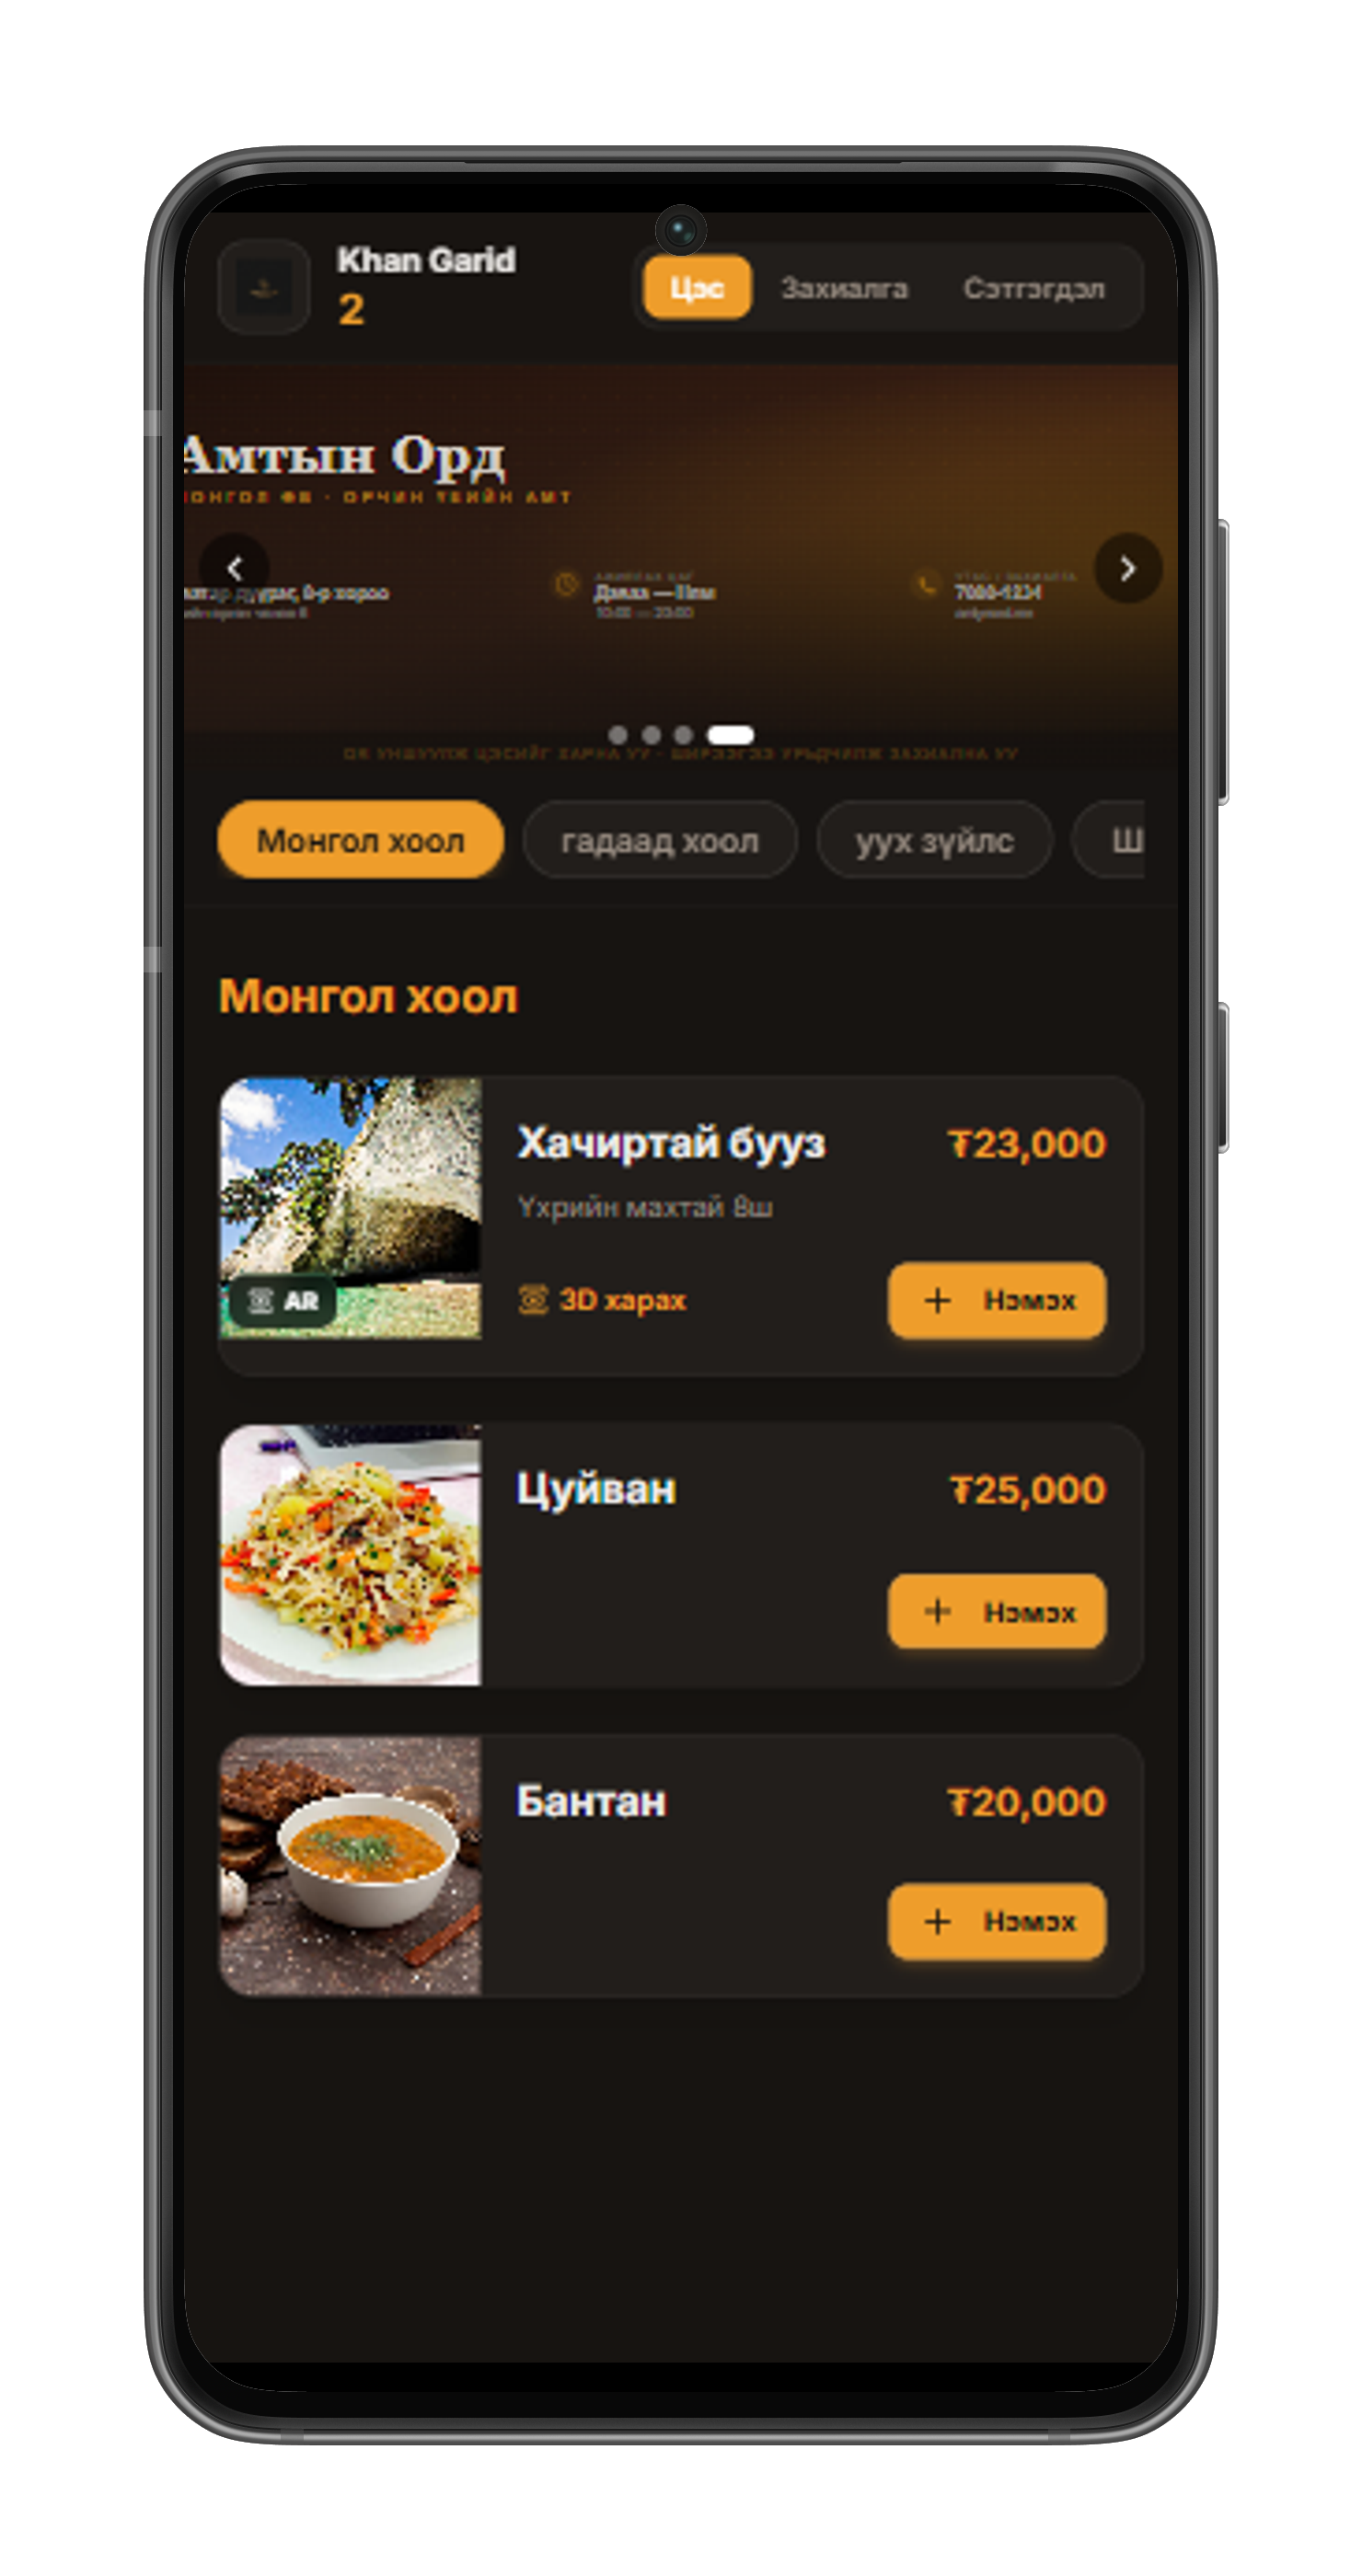
\includegraphics[width=0.45\textwidth]{Figures/guest-menu.png}
\caption{Зочны цэсийн дэлгэцийн дүрс (мобайл харагдац)}
\label{fig:guest-menu}
\end{figure}

\begin{figure}[htbp]
\centering
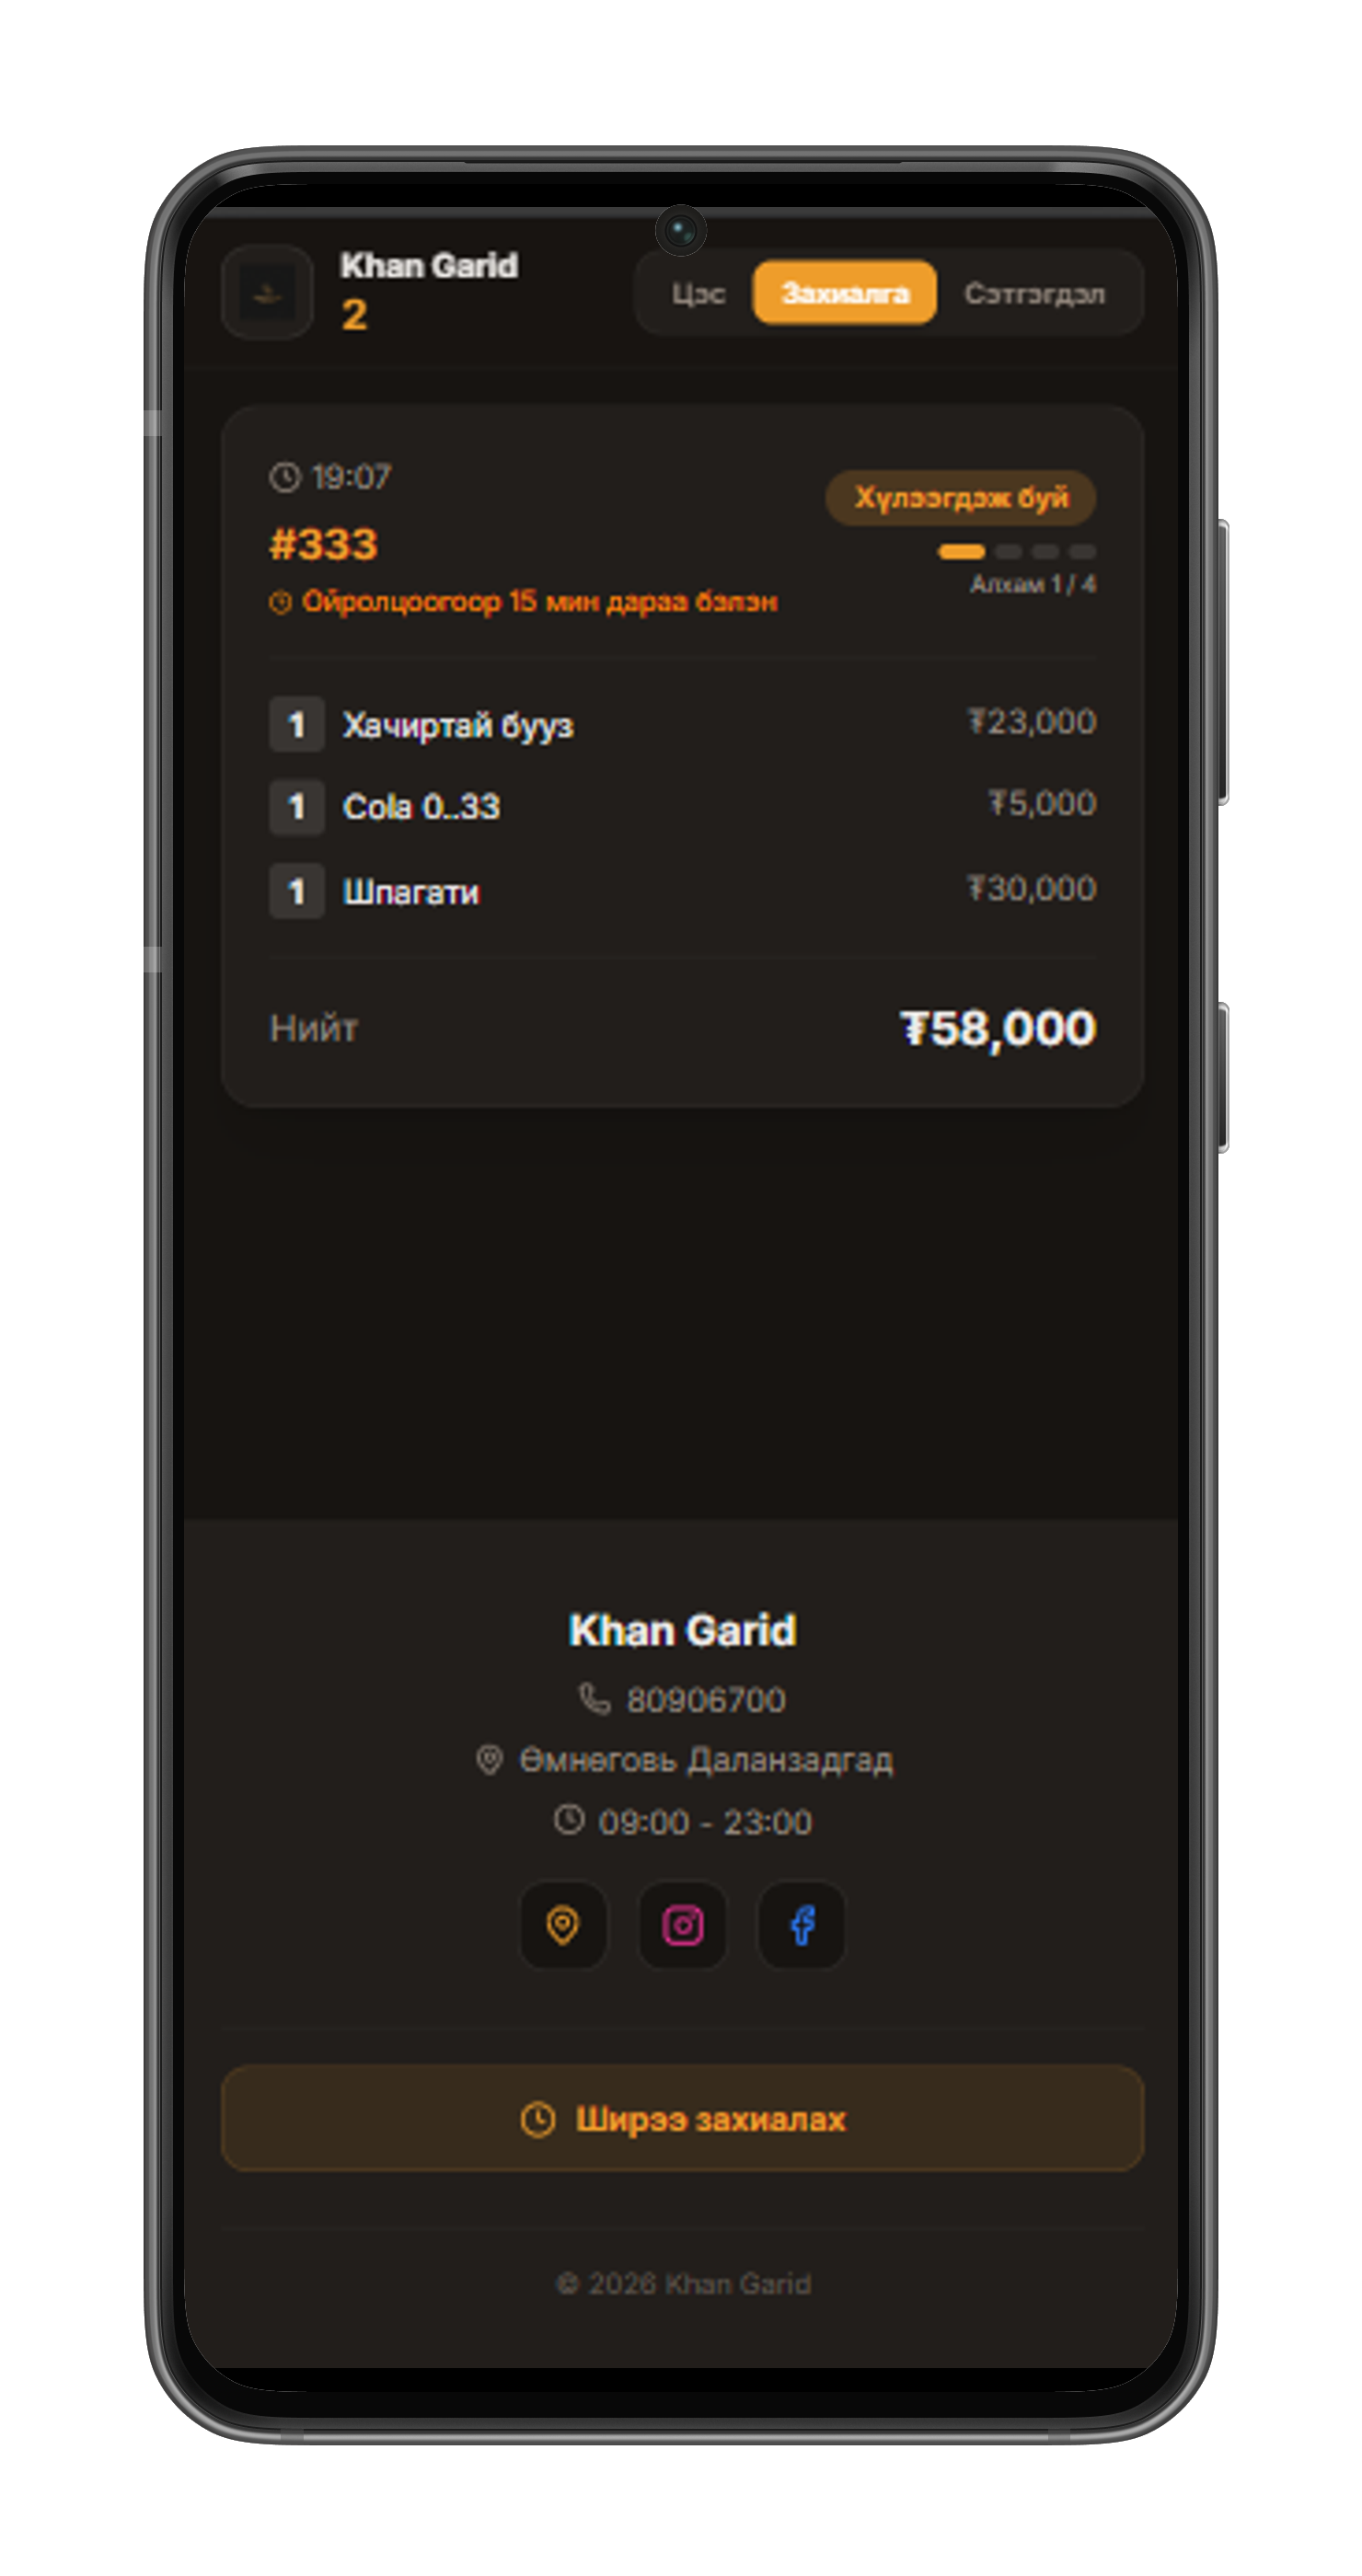
\includegraphics[width=0.45\textwidth]{Figures/guest-cart.png}
\caption{Зочны сагсны дэлгэц -- хоол сонгон захиалга өгөх}
\label{fig:guest-cart}
\end{figure}

\begin{figure}[htbp]
\centering
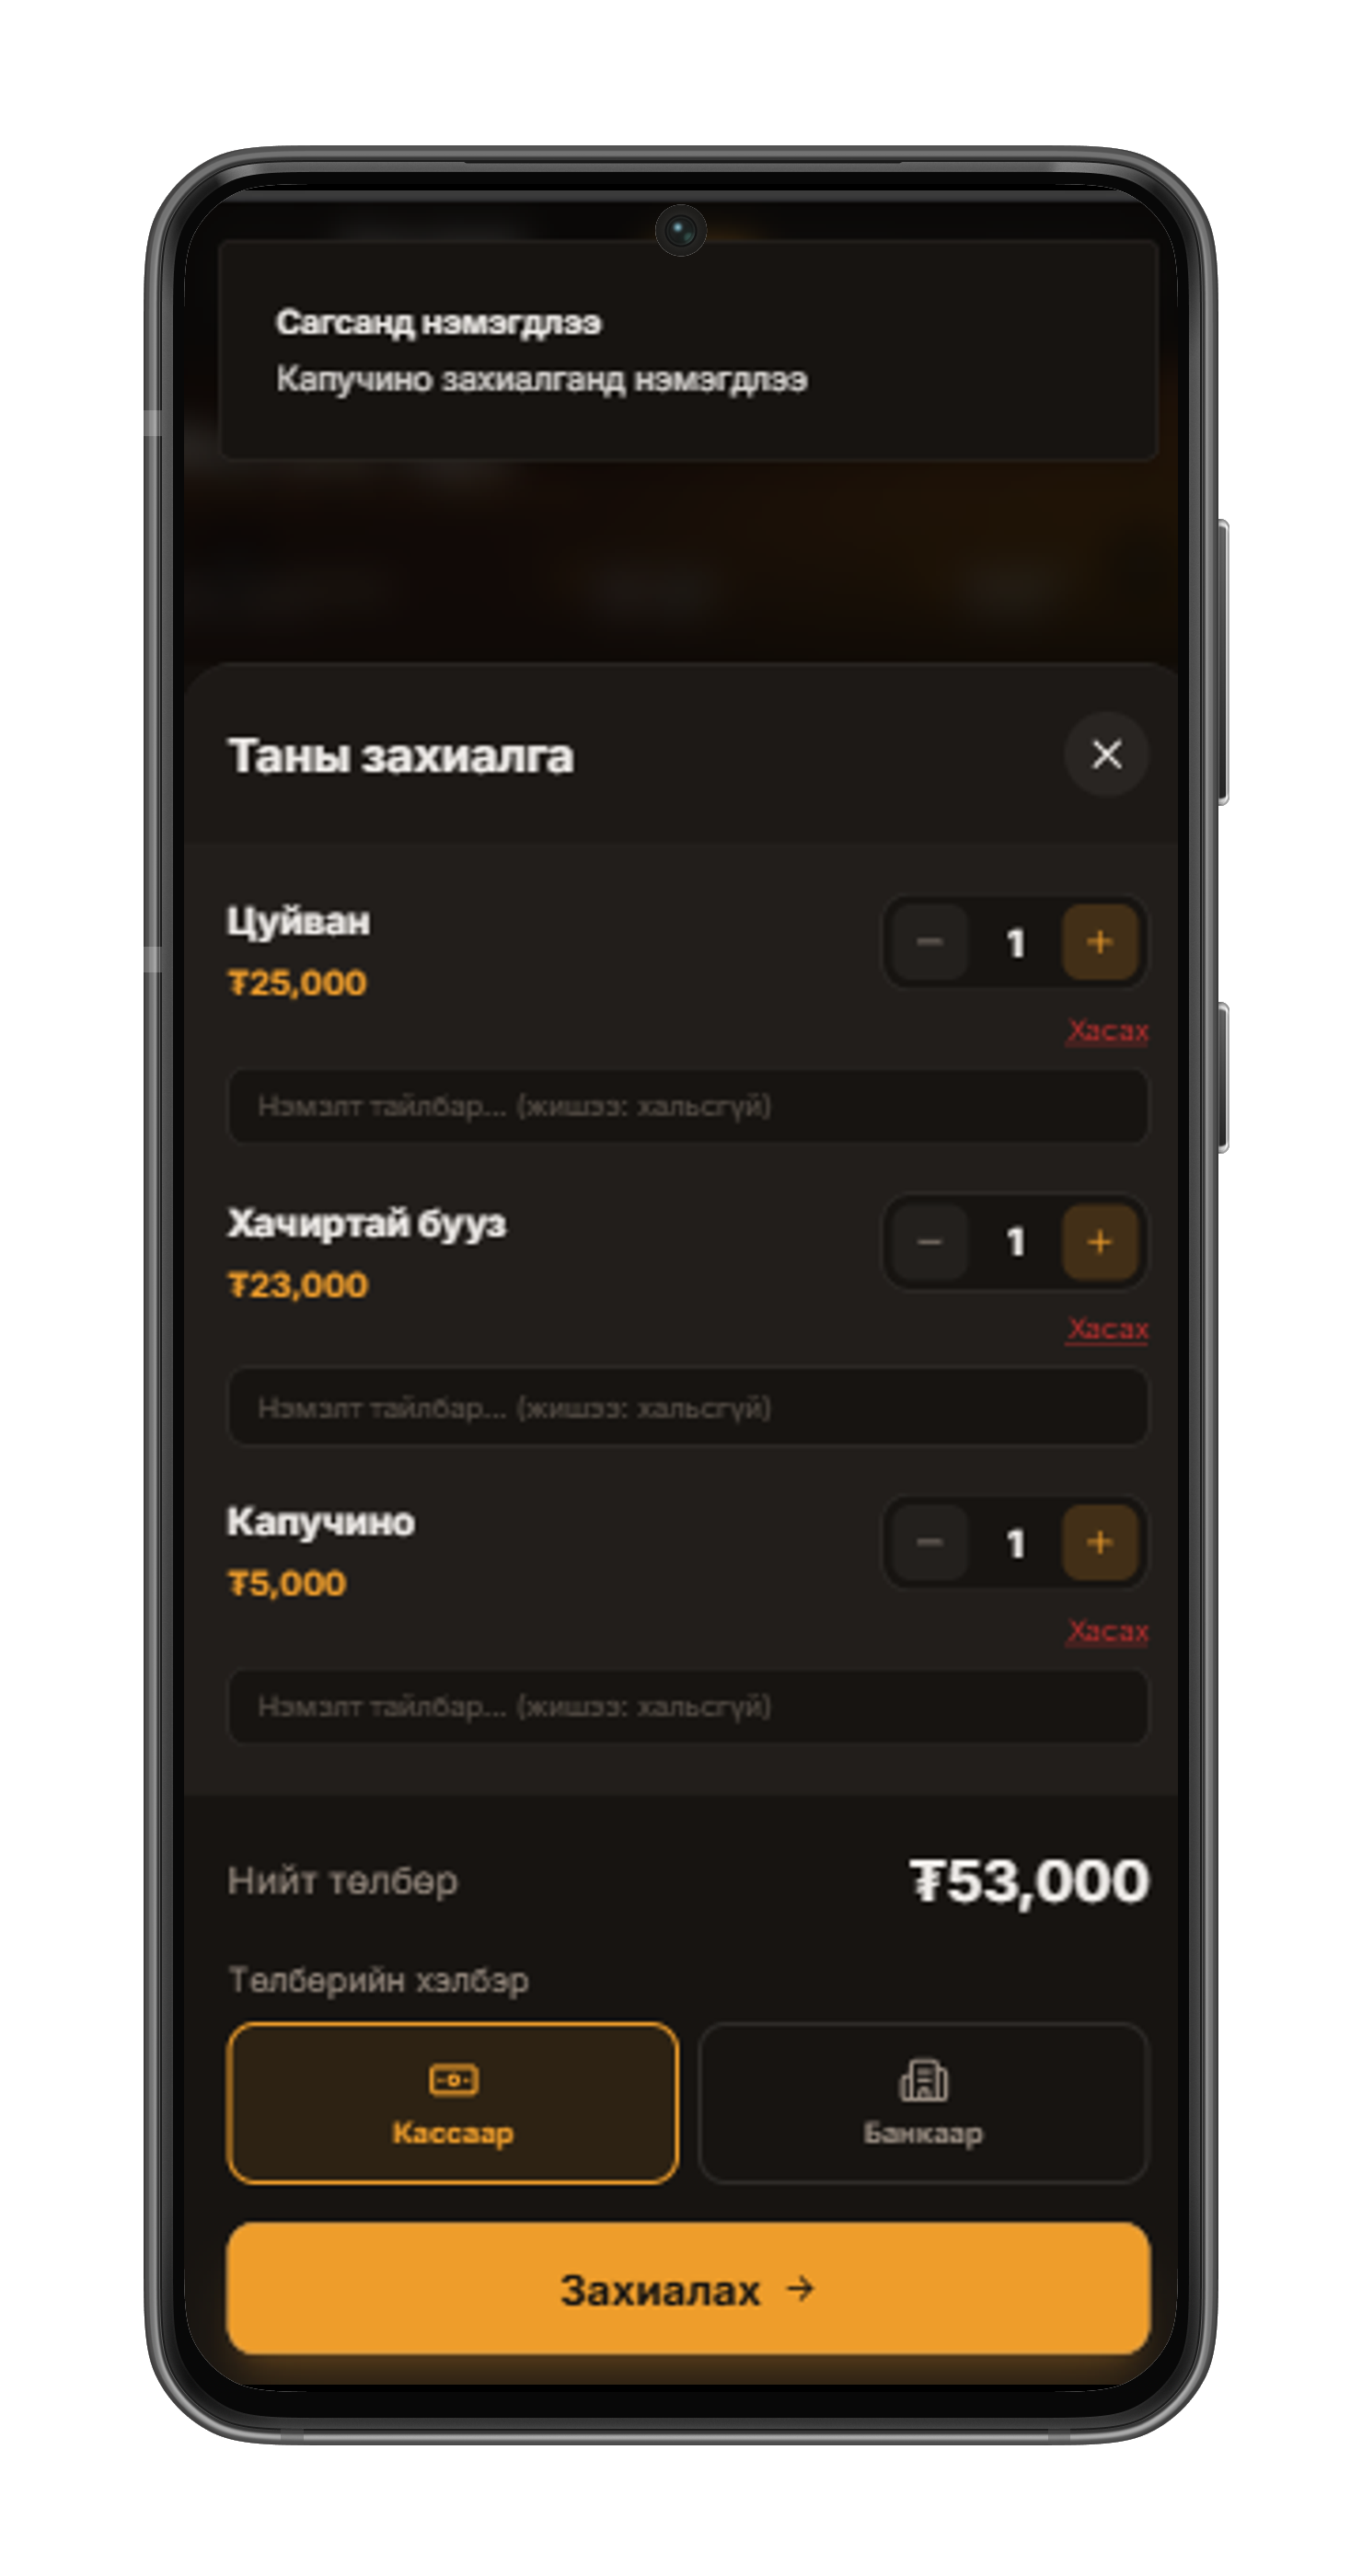
\includegraphics[width=0.45\textwidth]{Figures/guest-order-status.png}
\caption{Зочны захиалгын статус хянах дэлгэц}
\label{fig:guest-status}
\end{figure}

\subsection{Ажилтны удирдлагын самбар}

Ажилтны дэлгэц нь дараах модулиудтай:

\begin{itemize}
  \item \textbf{Захиалгын самбар}: Бодит цагийн захиалгын жагсаалт, статус шилжүүлгээ;
  \item \textbf{Ширээний удирдлага}: Ширээ нэмэх, засах, QR код хэвлэх;
  \item \textbf{Цэс удирдлага}: Ангилал, хоолны CRUD (Create, Read, Update, Delete);
  \item \textbf{Тайлан}: Өдрийн орлого, эрэлттэй хоол, ширээний статистик.
\end{itemize}

\begin{figure}[htbp]
\centering
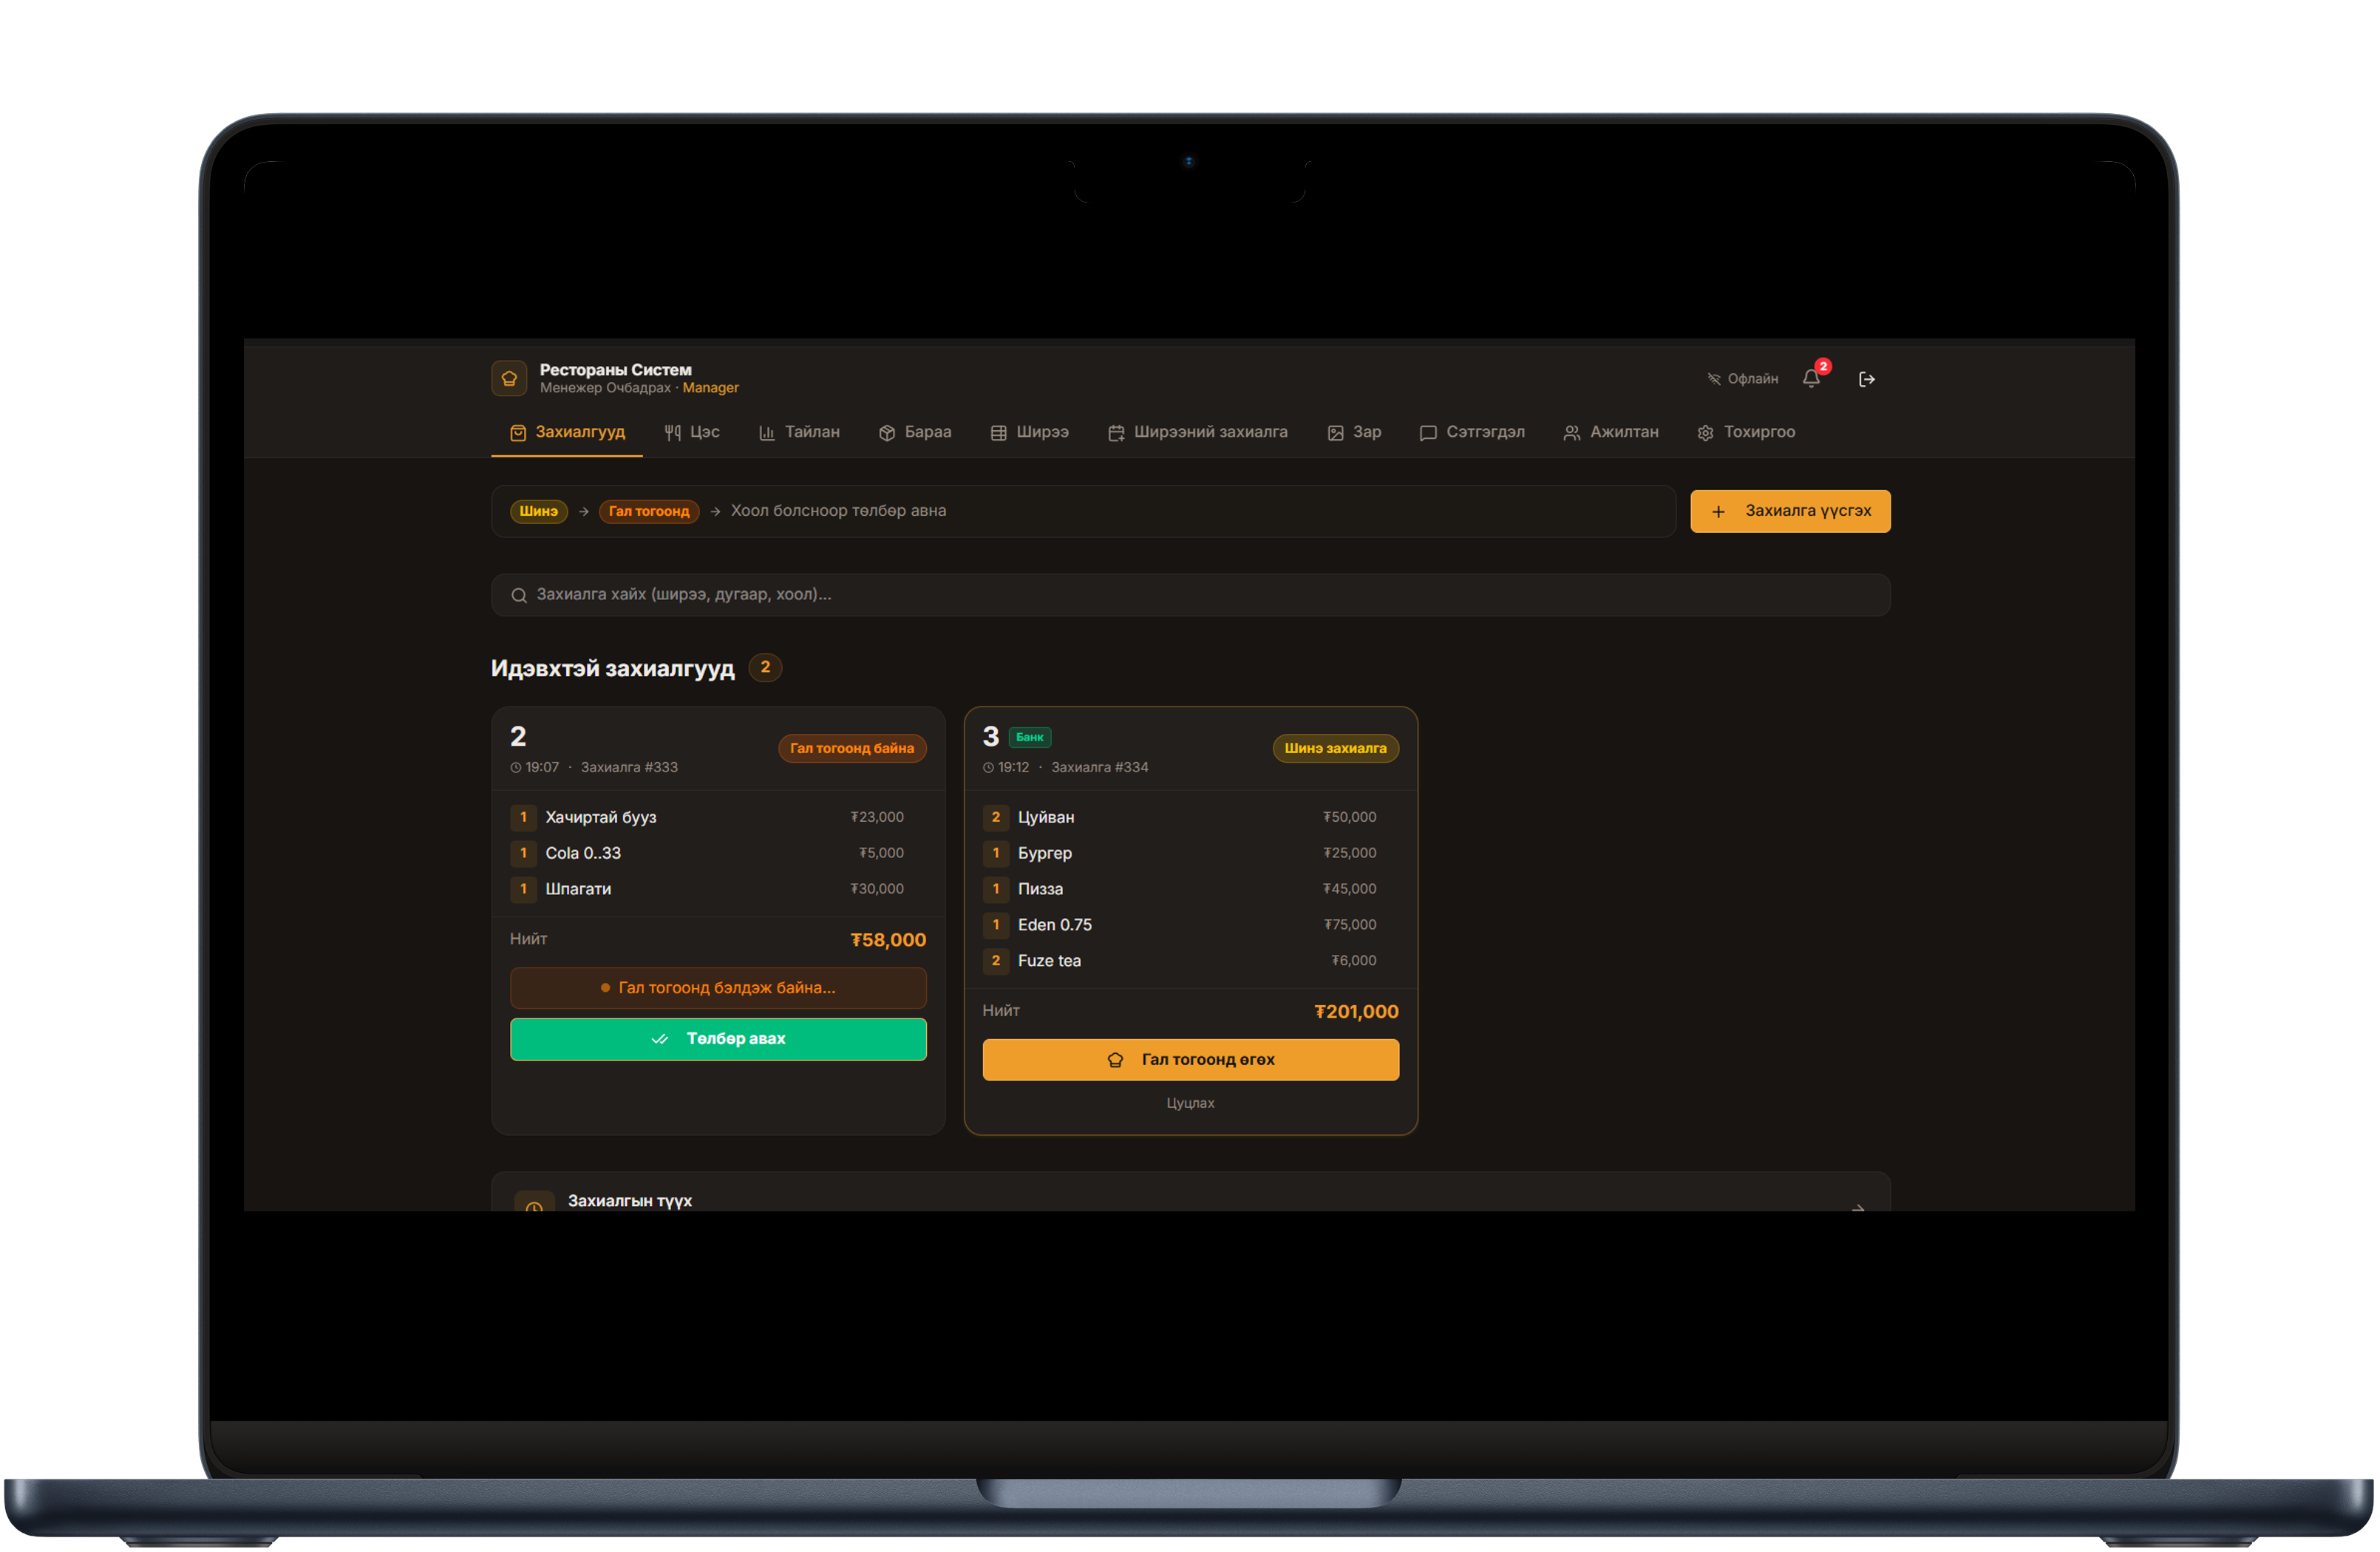
\includegraphics[width=0.95\textwidth]{Figures/staff-dashboard.png}
\caption{Ажилтны захиалгын удирдлагын самбар}
\label{fig:staff-dashboard}
\end{figure}

\begin{figure}[htbp]
\centering
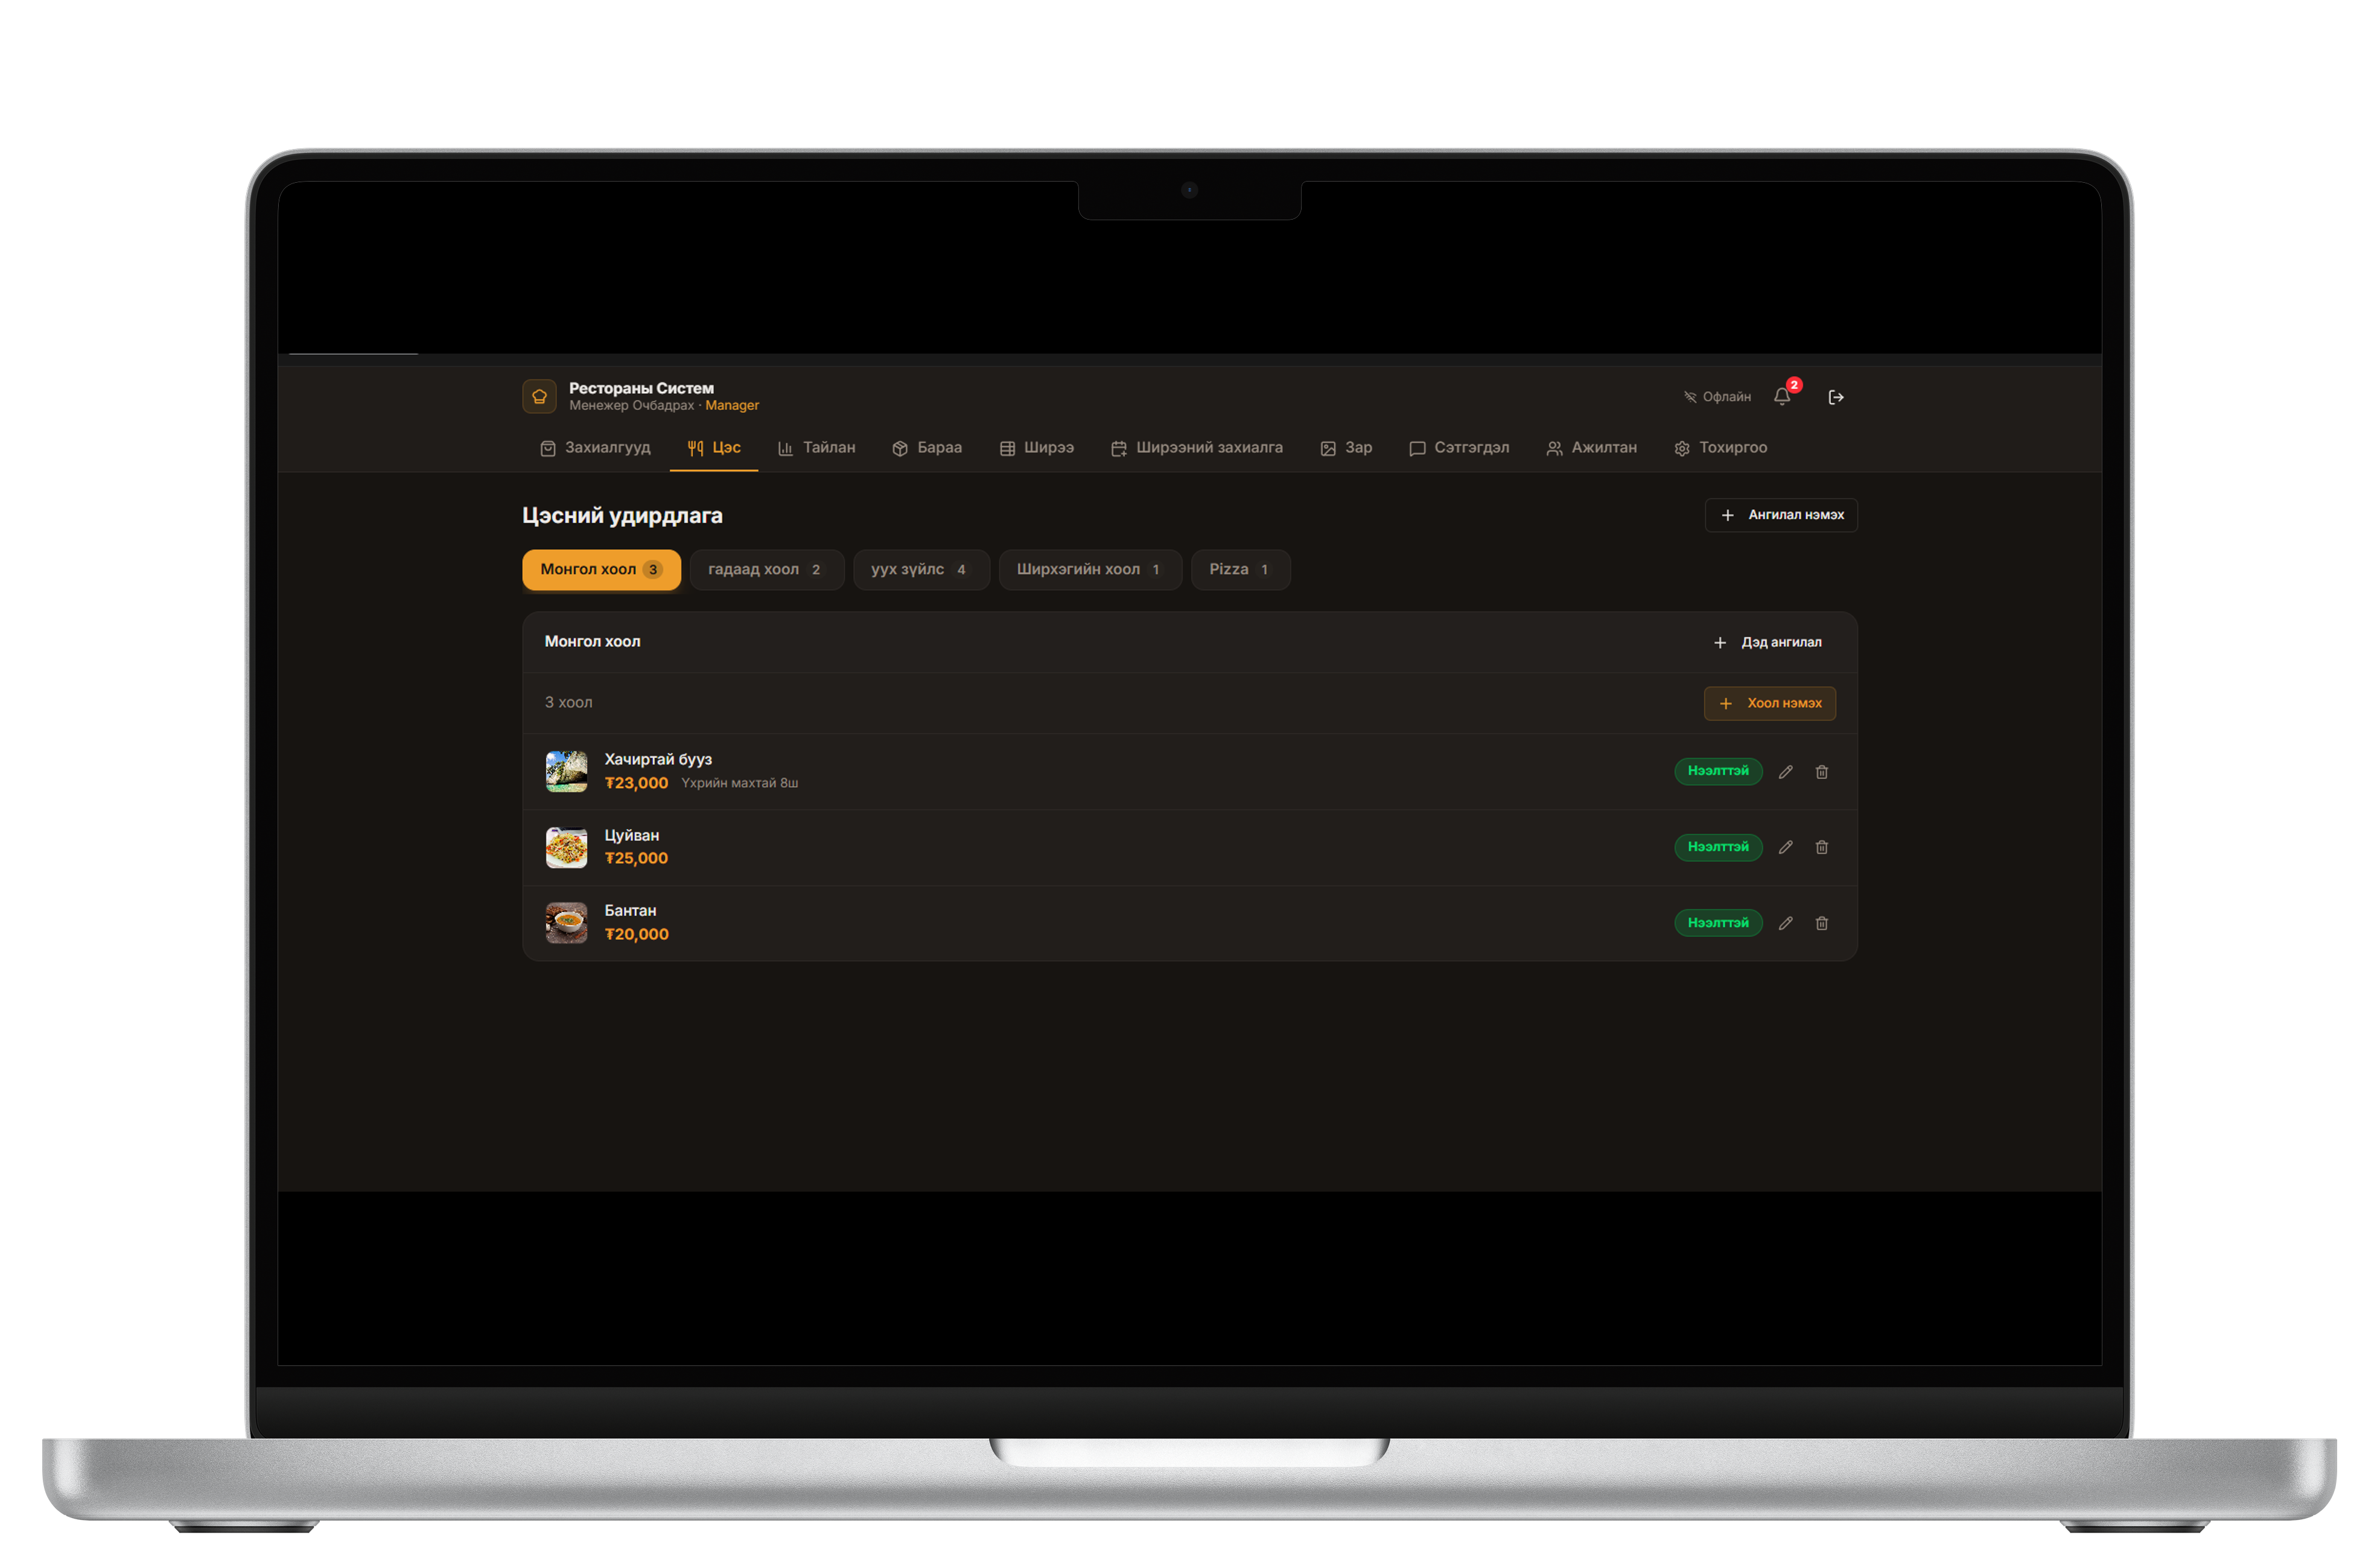
\includegraphics[width=0.95\textwidth]{Figures/staff-menu-manage.png}
\caption{Цэс удирдлагын дэлгэц -- хоол нэмэх, засах}
\label{fig:staff-menu}
\end{figure}

\begin{figure}[htbp]
\centering
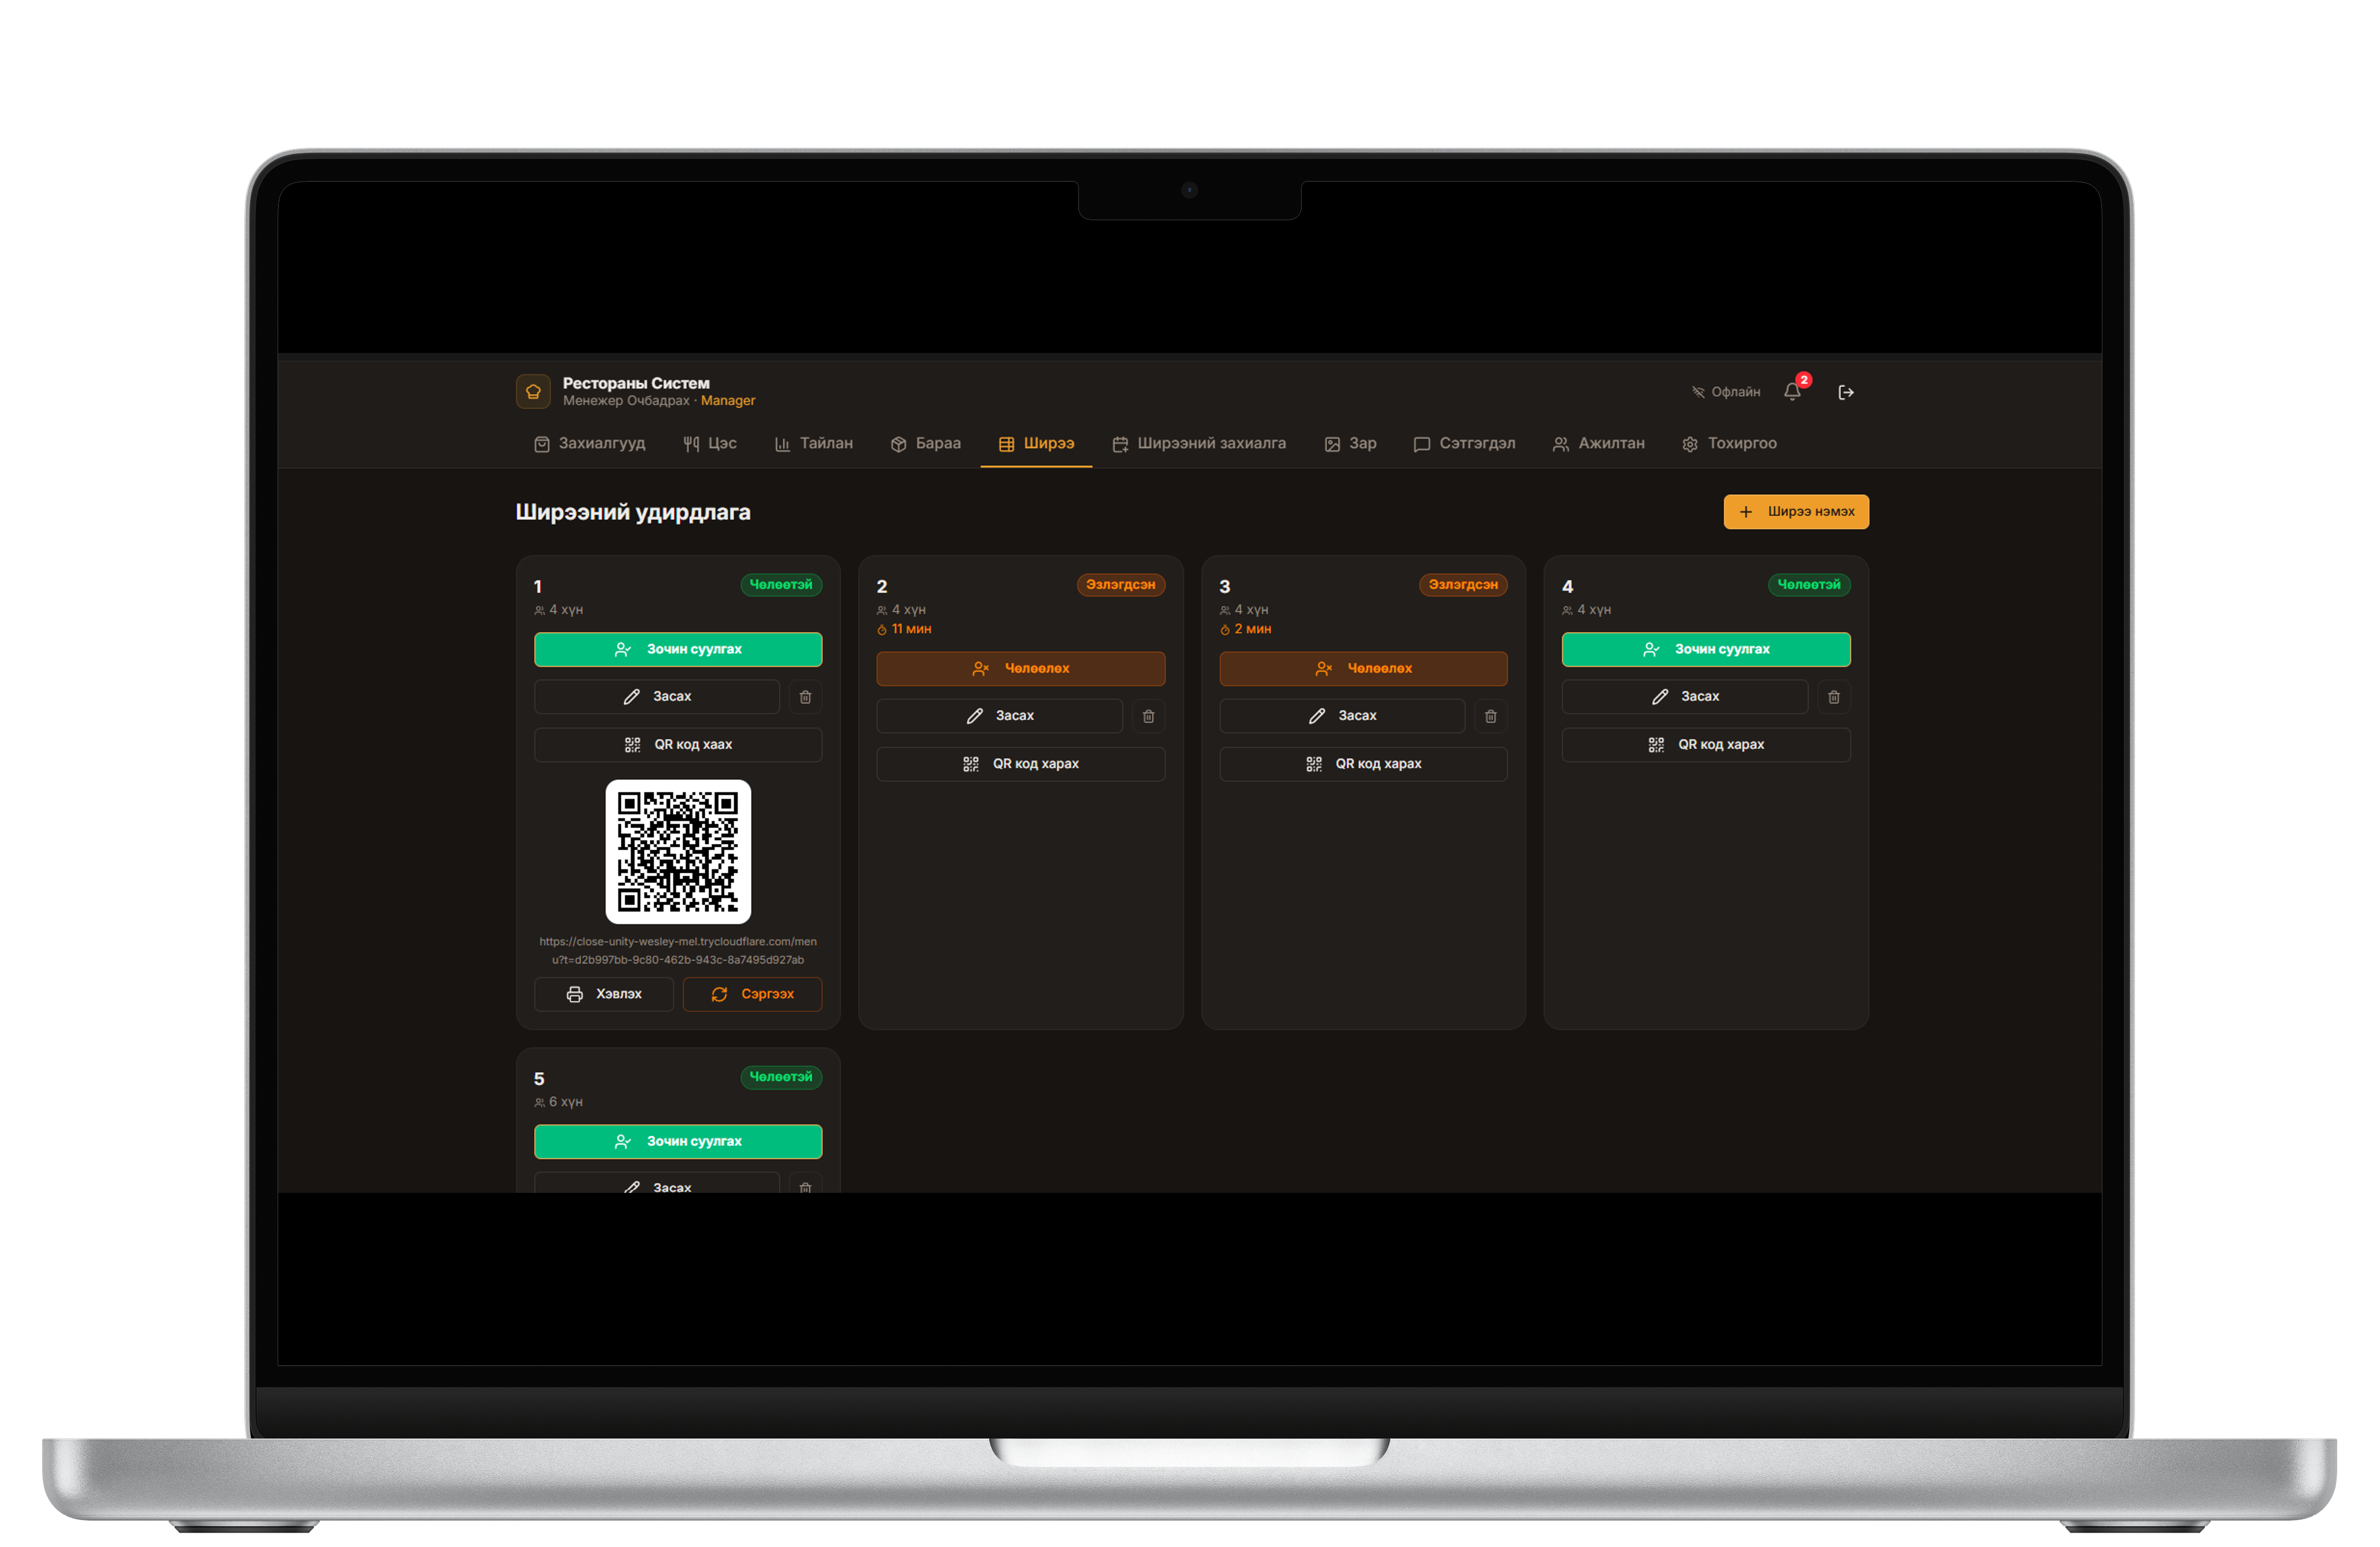
\includegraphics[width=0.95\textwidth]{Figures/staff-tables.png}
\caption{Ширээний удирдлага -- ширээ нэмэх, QR код хэвлэх}
\label{fig:staff-tables}
\end{figure}

\begin{figure}[htbp]
\centering
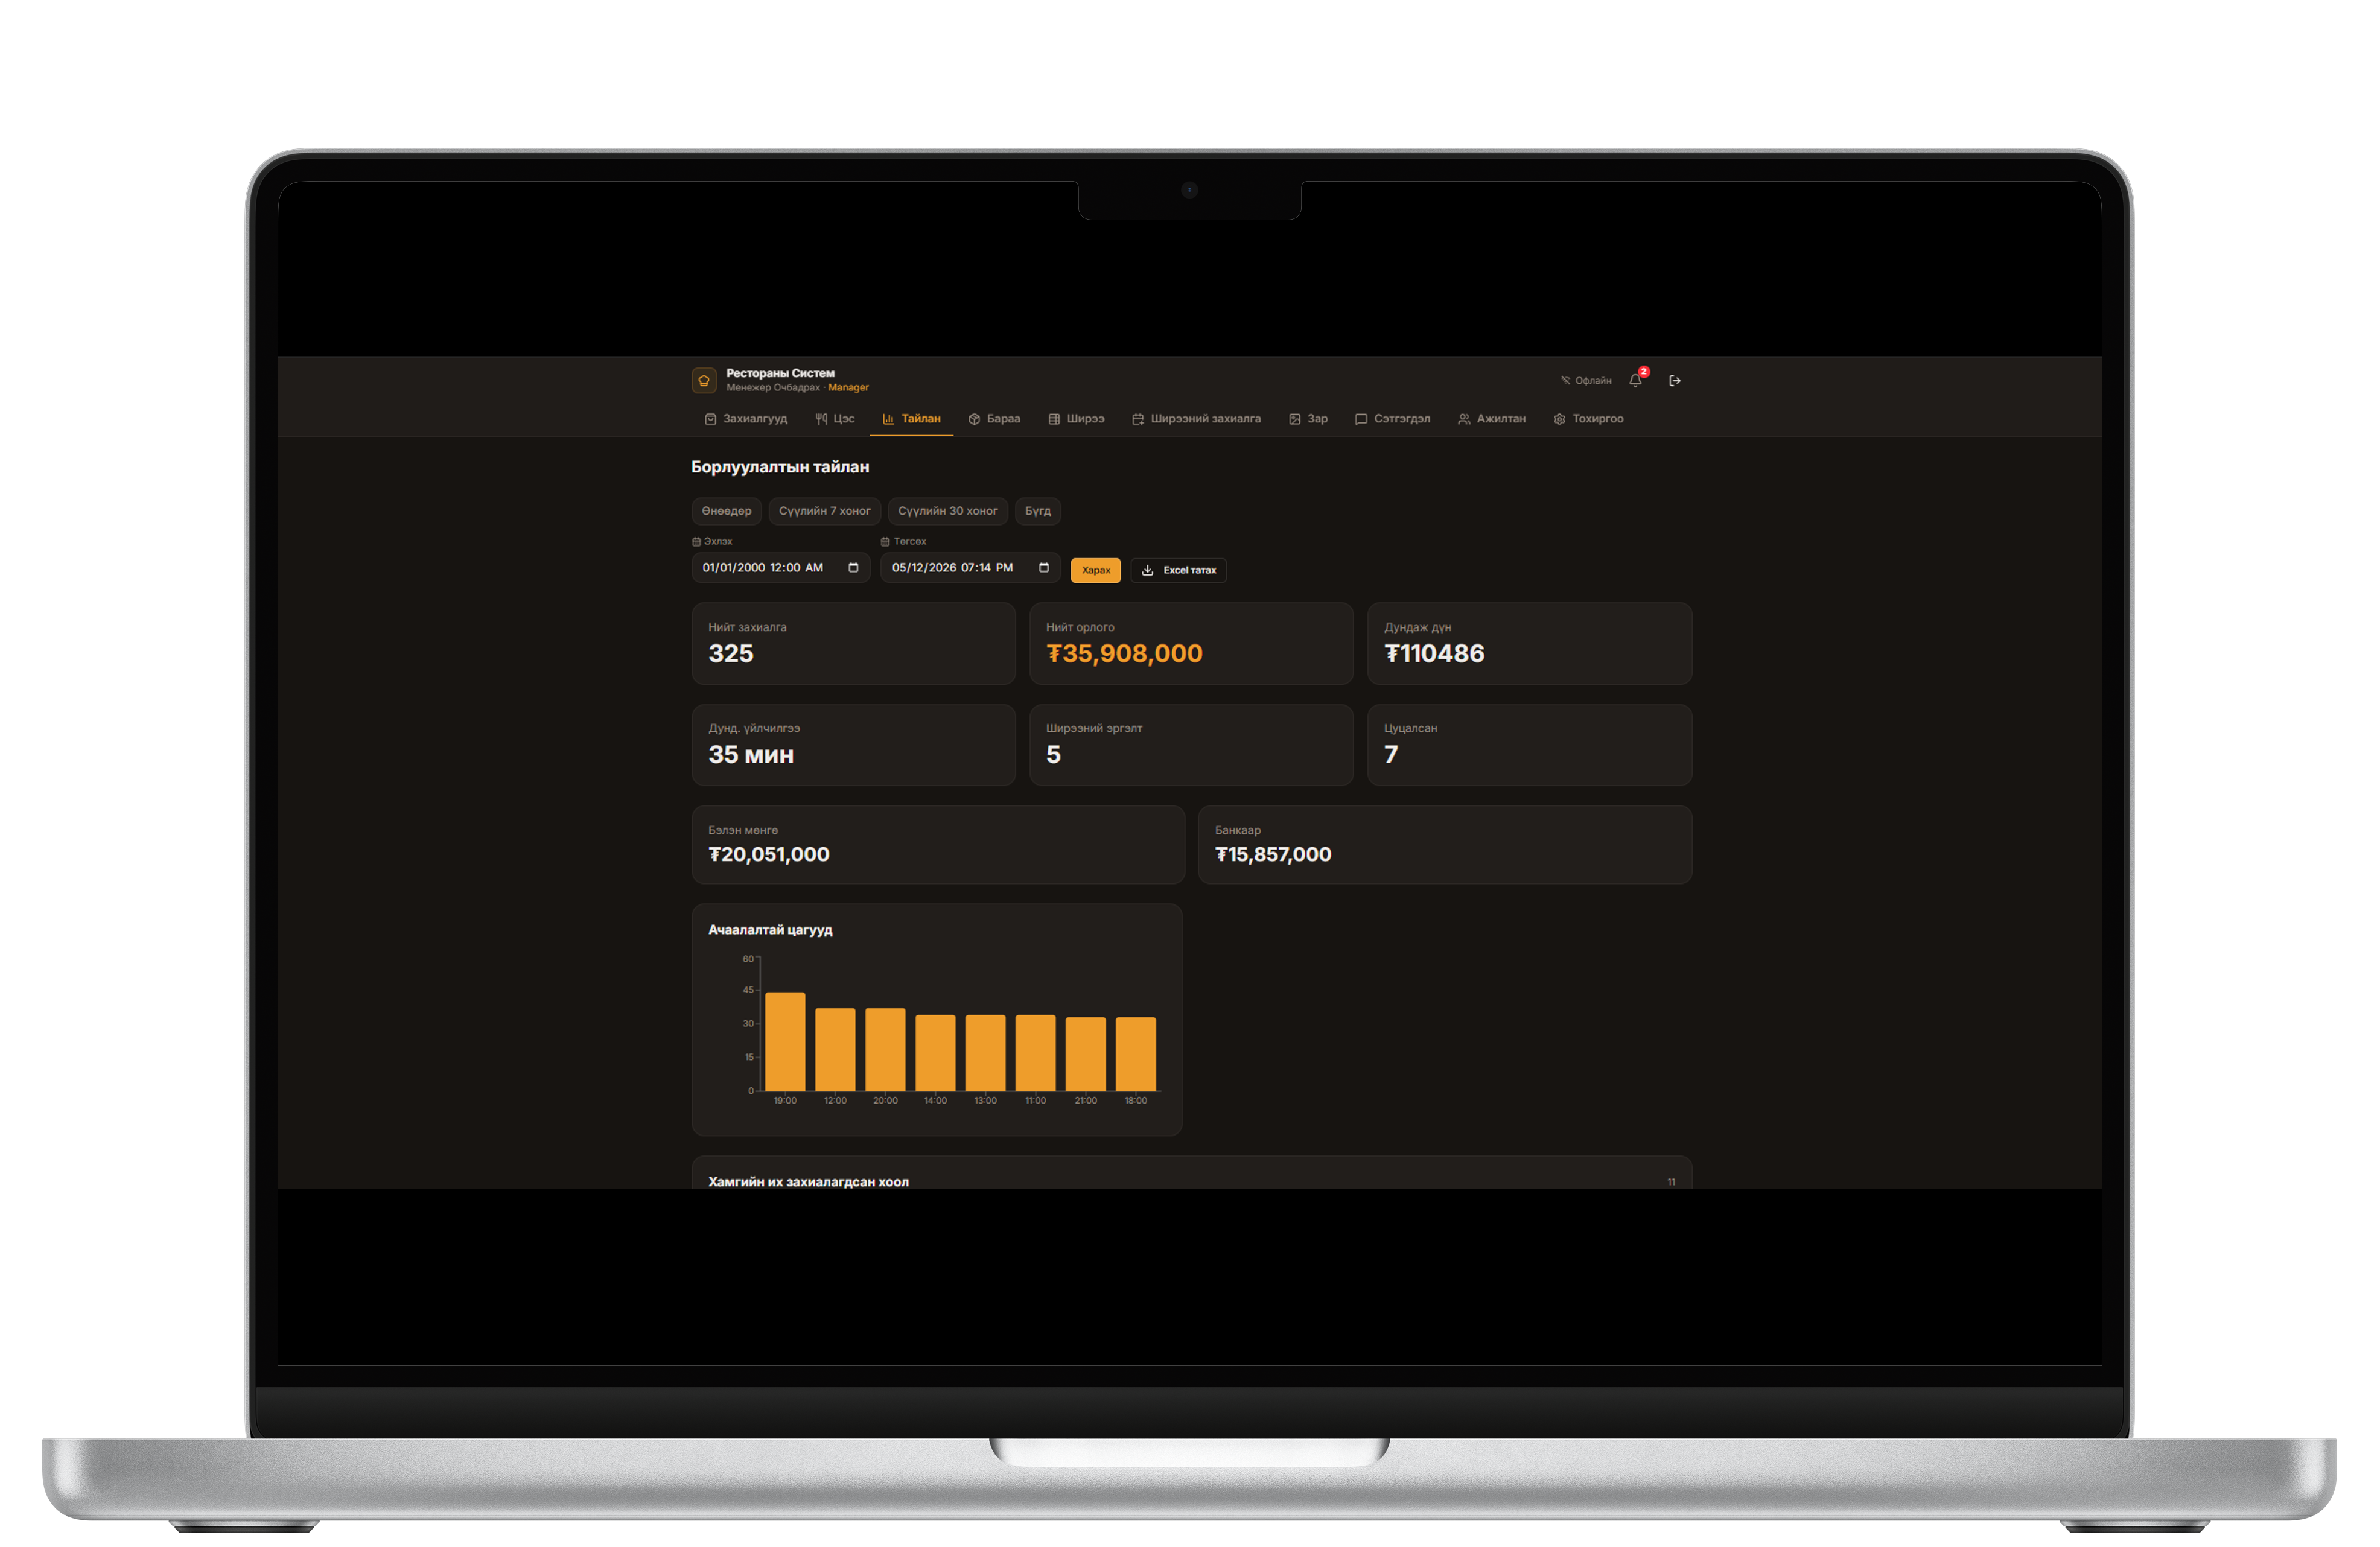
\includegraphics[width=0.95\textwidth]{Figures/staff-reports.png}
\caption{Тайлангийн дэлгэц -- өдрийн орлого, эрэлттэй хоол}
\label{fig:staff-reports}
\end{figure}

\begin{figure}[htbp]
\centering
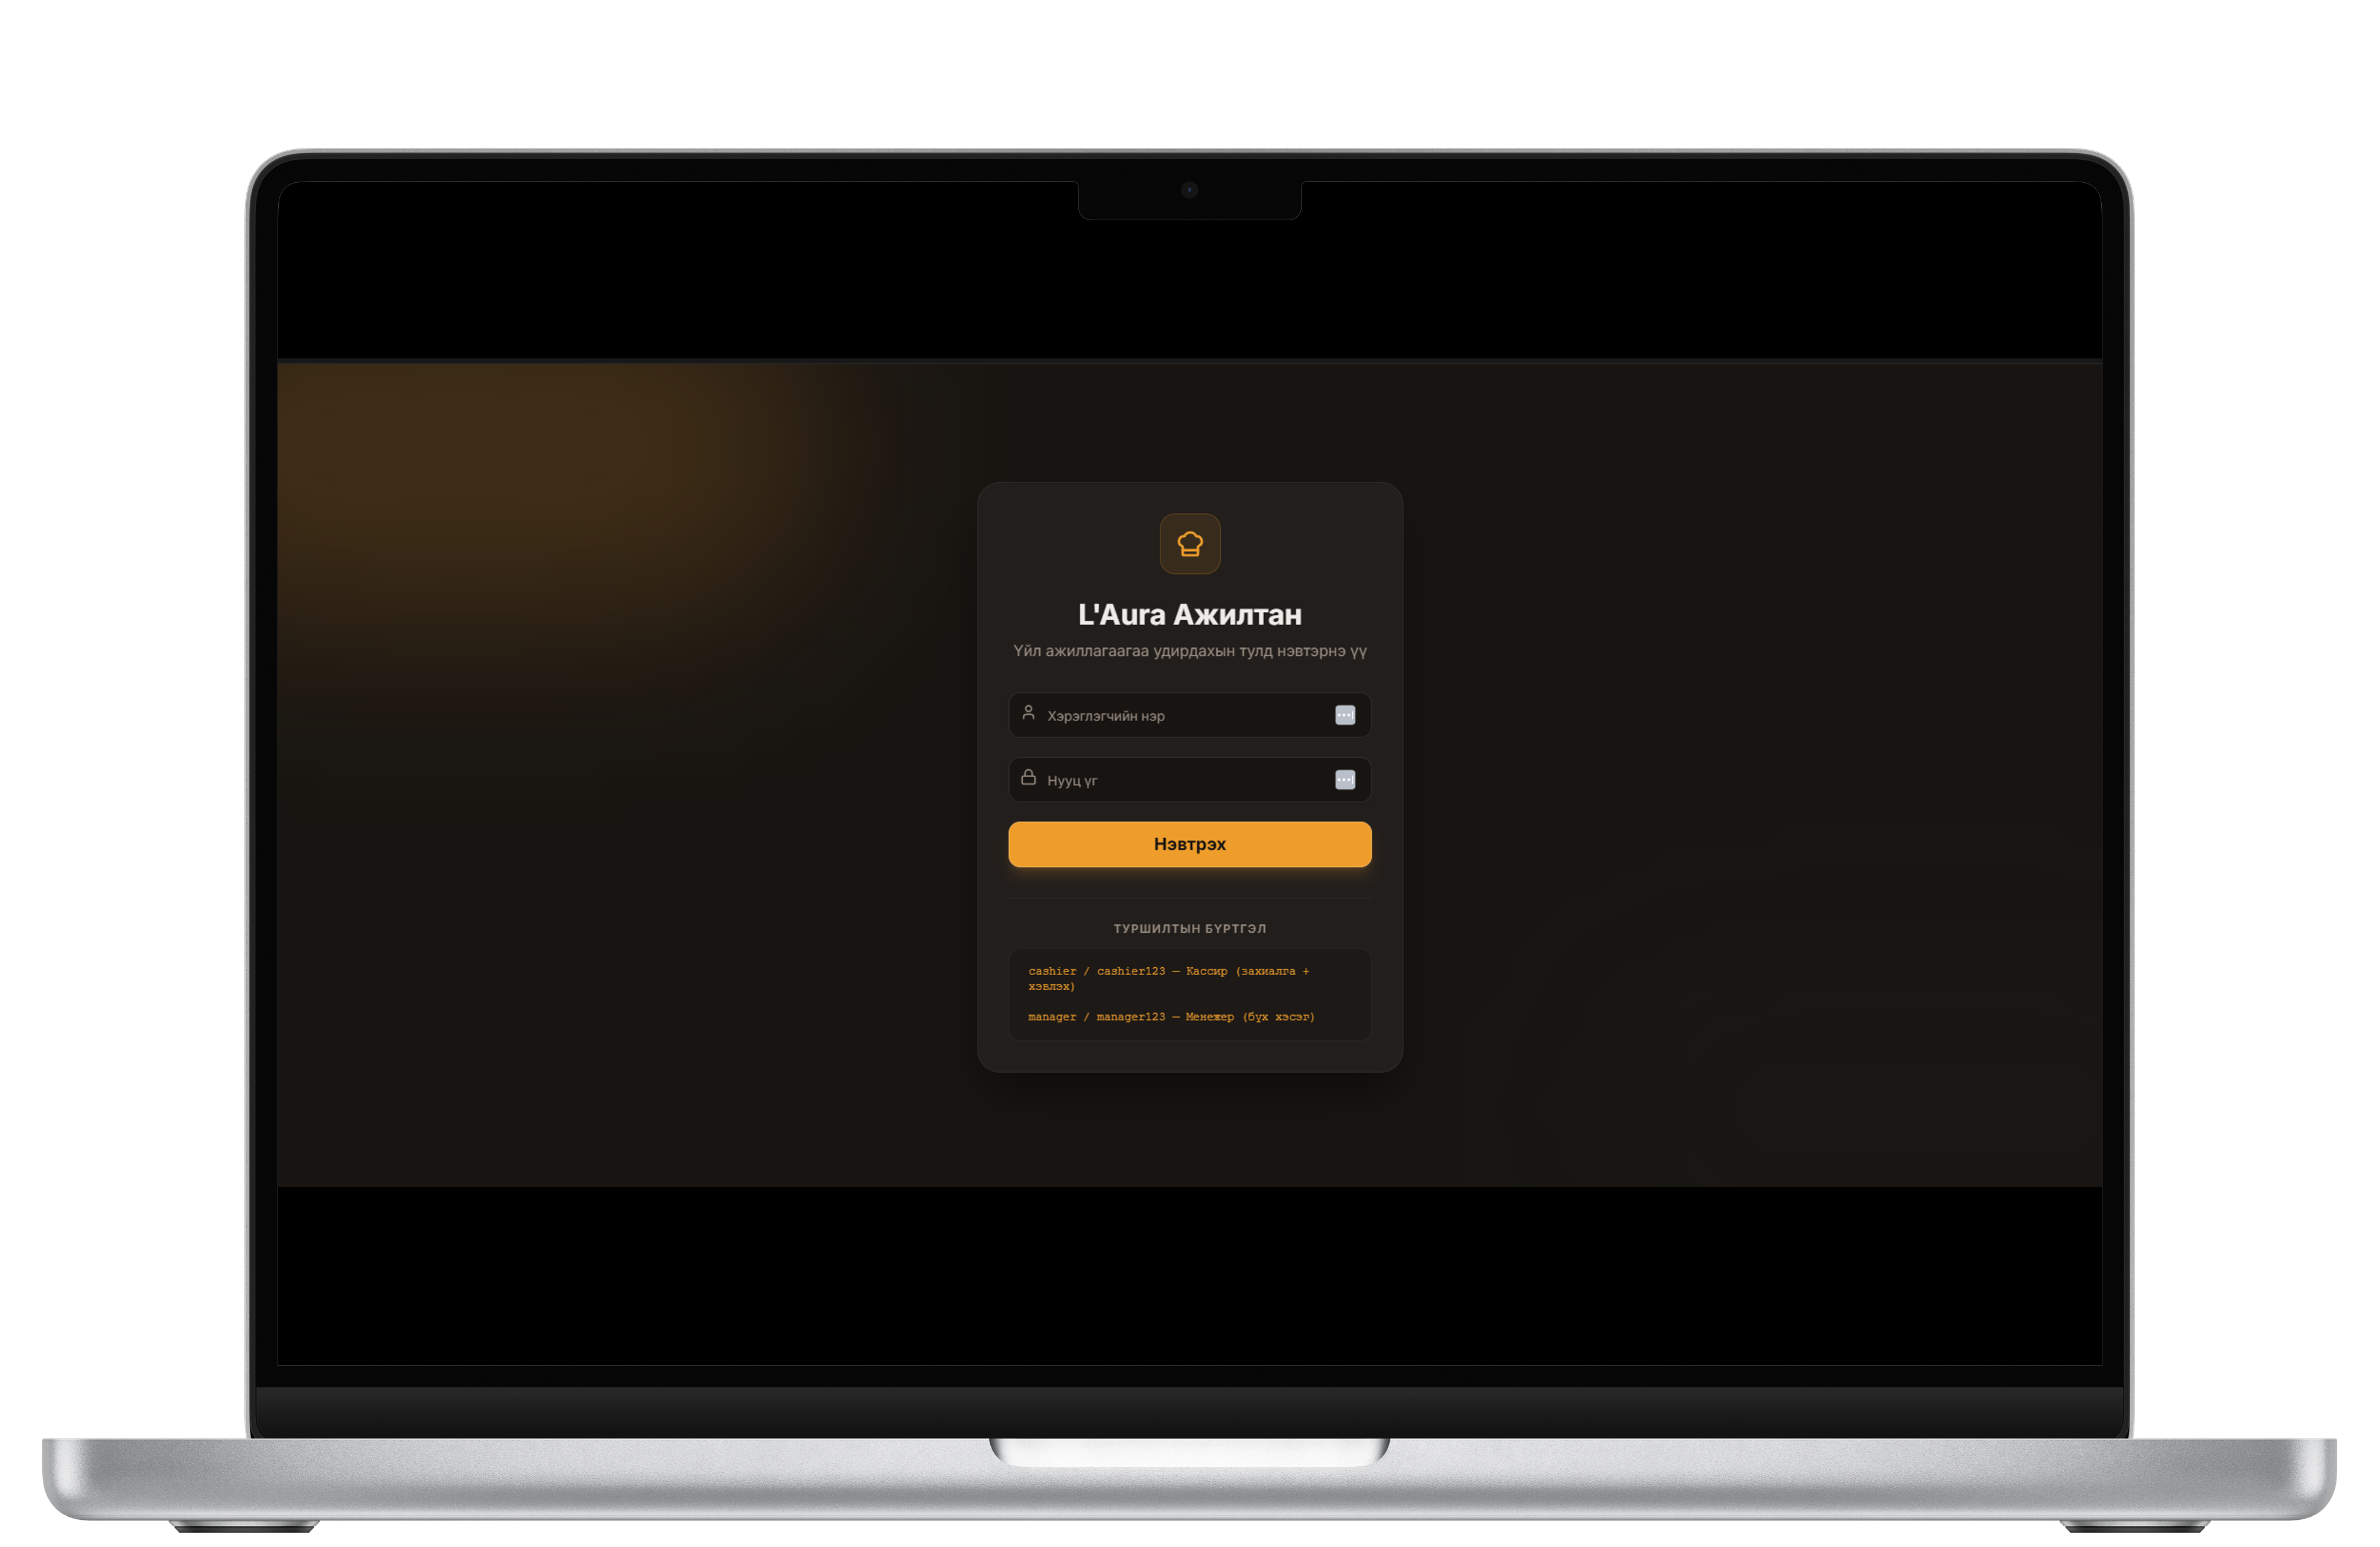
\includegraphics[width=0.95\textwidth]{Figures/login-page.png}
\caption{Ажилтны нэвтрэх дэлгэц}
\label{fig:login}
\end{figure}

\section{API жагсаалт}

Системийн REST API endpoint-уудыг бүлэг тус бүрээр (auth, menu, tables,
orders, inventory, reports, feedback, upload) нэгтгэн Хүснэгт~\ref{tab:api}
дээр харуулав.

\begin{longtable}{|c|l|l|p{5cm}|}
\caption{REST API endpoint-уудын жагсаалт} \label{tab:api} \\
\hline
\rowcolor{TableHdr}
\textcolor{white}{\textbf{No}} &
\textcolor{white}{\textbf{Метод}} &
\textcolor{white}{\textbf{Endpoint}} &
\textcolor{white}{\textbf{Тодорхойлолт}} \\ \hline
\endfirsthead
\hline
\rowcolor{TableHdr}
\textcolor{white}{\textbf{No}} &
\textcolor{white}{\textbf{Метод}} &
\textcolor{white}{\textbf{Endpoint}} &
\textcolor{white}{\textbf{Тодорхойлолт}} \\ \hline
\endhead

\multicolumn{4}{|l|}{\textbf{Auth}} \\ \hline
1 & POST & /api/auth/login & Нэвтрэх, JWT авах \\ \hline
\rowcolor{LightBlue}
2 & POST & /api/auth/register & Шинэ хэрэглэгч (manager-only) \\ \hline
3 & GET  & /api/auth/me & Одоогийн хэрэглэгчийн мэдээлэл \\ \hline
\multicolumn{4}{|l|}{\textbf{Menu}} \\ \hline
4 & GET  & /api/menu & Цэс (ангиллаар) \\ \hline
\rowcolor{LightBlue}
5 & GET  & /api/menu/categories & Ангиллын жагсаалт \\ \hline
6 & POST & /api/menu & Шинэ хоол нэмэх \\ \hline
\rowcolor{LightBlue}
7 & PUT  & /api/menu/:id & Хоолны мэдээлэл засах \\ \hline
8 & DELETE & /api/menu/:id & Хоол устгах \\ \hline
\multicolumn{4}{|l|}{\textbf{Tables}} \\ \hline
\rowcolor{LightBlue}
9 & GET  & /api/tables & Ширээний жагсаалт \\ \hline
10 & GET  & /api/tables/:token & QR token-оор ширээ \\ \hline
\rowcolor{LightBlue}
11 & POST & /api/tables & Шинэ ширээ \\ \hline
12 & PUT  & /api/tables/:id & Ширээ засах \\ \hline
\rowcolor{LightBlue}
13 & DELETE & /api/tables/:id & Ширээ устгах \\ \hline
14 & GET  & /api/tables/:id/qr & QR PNG татах \\ \hline
\multicolumn{4}{|l|}{\textbf{Orders}} \\ \hline
\rowcolor{LightBlue}
15 & GET  & /api/orders & Бүх захиалга \\ \hline
16 & GET  & /api/orders/:id & Нэг захиалгын дэлгэрэнгүй \\ \hline
\rowcolor{LightBlue}
17 & POST & /api/orders & Шинэ захиалга \\ \hline
18 & PATCH & /api/orders/:id & Статус шинэчлэх \\ \hline
\rowcolor{LightBlue}
19 & DELETE & /api/orders/:id & Захиалга цуцлах \\ \hline
\multicolumn{4}{|l|}{\textbf{Inventory}} \\ \hline
20 & GET  & /api/inventory & Нөөцийн бараа \\ \hline
\rowcolor{LightBlue}
21 & POST & /api/inventory & Шинэ бараа + менюнд нэмэх \\ \hline
22 & PATCH & /api/inventory/:id & Бараа засварлах \\ \hline
\rowcolor{LightBlue}
23 & DELETE & /api/inventory/:id & Бараа устгах (soft/hard) \\ \hline
\multicolumn{4}{|l|}{\textbf{Reports}} \\ \hline
24 & GET  & /api/reports/daily & Өдрийн орлого \\ \hline
\rowcolor{LightBlue}
25 & GET  & /api/reports/popular & Эрэлттэй хоол ТОП-10 \\ \hline
26 & GET  & /api/reports/low-stock & Доод хэмжээнд хүрсэн нөөц \\ \hline
\multicolumn{4}{|l|}{\textbf{Feedback ба бусад}} \\ \hline
\rowcolor{LightBlue}
27 & POST & /api/feedback & Зочны сэтгэгдэл илгээх \\ \hline
28 & GET  & /api/feedback & Менежерт сэтгэгдлүүд \\ \hline
\rowcolor{LightBlue}
29 & PATCH & /api/feedback/:id/read & Сэтгэгдэл уншсан тэмдэглэх \\ \hline
30 & POST & /api/upload & Зураг байршуулах (S3) \\ \hline

\end{longtable}

\section{Socket.IO үйл явдлууд}

Бодит цагийн харилцааны Socket.IO үйл явдлуудыг Хүснэгт~\ref{tab:socket} дээр
харуулав.

\begin{table}[htbp]
\caption{Socket.IO үйл явдлуудын жагсаалт}
\label{tab:socket}
\centering
\small
\begin{tabularx}{\textwidth}{|c|L|L|Y|}
\hline
\rowcolor{TableHdr}
\textcolor{white}{\textbf{No}} &
\textcolor{white}{\textbf{Үйл явдал}} &
\textcolor{white}{\textbf{Чиглэл}} &
\textcolor{white}{\textbf{Тодорхойлолт}} \\ \hline
1 & connect & Клиент $\to$ Сервер & Socket холболт тогтоох \\ \hline
\rowcolor{LightBlue}
2 & join\_room & Клиент $\to$ Сервер & restaurant\_1 эсвэл ширээний room-д нэгдэх \\ \hline
3 & new\_order & Сервер $\to$ Ажилтан & Шинэ захиалга broadcast \\ \hline
\rowcolor{LightBlue}
4 & order\_update & Сервер $\to$ Клиент & Захиалгын статус шинэчлэлт \\ \hline
5 & order\_confirmed & Сервер $\to$ Зочин & Захиалга баталгаажсан мэдэгдэл \\ \hline
\rowcolor{LightBlue}
6 & table\_update & Сервер $\to$ Клиент & Ширээний статус шинэчлэлт \\ \hline
7 & low\_stock & Сервер $\to$ Менежер & Нөөц доод хэмжээнд хүрсэн \\ \hline
\rowcolor{LightBlue}
8 & new\_feedback & Сервер $\to$ Менежер & Зочноос сэтгэгдэл ирсэн \\ \hline
9 & disconnect & Клиент $\to$ Сервер & Холболт тасрах \\ \hline
\end{tabularx}
\end{table}

\section{Гүйцэтгэлийн туршилт}

\subsection{k6 ачааллын туршилт}

Системийн гүйцэтгэлийг k6 ачааллын туршилтын хэрэгслээр шалгасан. Туршилтын
тохиргоо: 200 виртуал хэрэглэгч (VU), 5 минутын хугацаа, ramp-up 30 секунд.

\begin{table}[htbp]
\caption{k6 ачааллын туршилтын үр дүн}
\label{tab:k6}
\centering
\small
\begin{tabularx}{\textwidth}{|L|Y|Y|Y|}
\hline
\rowcolor{TableHdr}
\textcolor{white}{\textbf{Endpoint}} &
\textcolor{white}{\textbf{Дундаж (мс)}} &
\textcolor{white}{\textbf{p95 (мс)}} &
\textcolor{white}{\textbf{p99 (мс)}} \\ \hline
GET /api/menu & 45 & 89 & 134 \\ \hline
\rowcolor{LightBlue}
GET /api/tables/:token & 38 & 72 & 112 \\ \hline
POST /api/orders & 120 & 198 & 287 \\ \hline
\rowcolor{LightBlue}
PATCH /api/orders/:id & 85 & 156 & 223 \\ \hline
GET /api/reports/daily & 156 & 245 & 312 \\ \hline
\rowcolor{LightBlue}
WebSocket мессеж & 45 & 78 & 98 \\ \hline
\end{tabularx}
\end{table}

Туршилтын үр дүнгээс харахад бүх endpoint-ийн дундаж хариу хугацаа 200 мс-ээс бага
байгаа нь функционал бус шаардлагыг (Хүснэгт~\ref{tab:nfr_perf}) бүрэн хангаж байна.
WebSocket мессежийн дамжуулалт 45 мс дунджаар буюу 100 мс-ээс бага шаардлагыг давж
хангасан.

\subsection{Ачааллын графикийн дүн шинжилгээ}

200 VU-ийн ачаалалд серверийн CPU ашиглалт дунджаар 35\%, санах ой (RAM) 512 MB
орчим байсан бөгөөд энэ нь серверийн доод шаардлага (2 CPU, 4 GB RAM)-ийн хүрээнд
тогтвортой ажиллаж байгааг харуулж байна.

\section{SUS (System Usability Scale) үнэлгээ}

Системийн хэрэглэхэд хялбар байдлыг үнэлэхийн тулд 28 хэрэглэгч (20 зочин + 4
кассир + 4 менежер)-ээр SUS стандарт асуулгын аргачлалаар үнэлгээ хийлгэсэн.

SUS нь John Brooke-ийн 1986 онд боловсруулсан 10 асуулт бүхий стандартчилсан
хэрэглэгчийн сэтгэл ханамжийн арга бөгөөд 0--100 оноогоор дүгнэгддэг~\cite{brooke1996}.

\begin{table}[htbp]
\caption{SUS үнэлгээний үр дүн}
\label{tab:sus}
\centering
\small
\begin{tabularx}{\textwidth}{|c|L|Y|}
\hline
\rowcolor{TableHdr}
\textcolor{white}{\textbf{No}} &
\textcolor{white}{\textbf{Асуулт}} &
\textcolor{white}{\textbf{Дундаж оноо}} \\ \hline
1 & Би энэ системийг байнга ашиглахыг хүснэ & 4.1 \\ \hline
\rowcolor{LightBlue}
2 & Систем хэт нарийн төвөгтэй санагдсан & 1.6 \\ \hline
3 & Системийг ашиглахад хялбар байсан & 4.3 \\ \hline
\rowcolor{LightBlue}
4 & Системийг ашиглахын тулд тусламж хэрэгтэй & 1.4 \\ \hline
5 & Системийн функцууд сайн нэгтгэгдсэн & 4.0 \\ \hline
\rowcolor{LightBlue}
6 & Системд хэт их зөрчил байна & 1.5 \\ \hline
7 & Ихэнх хүмүүс хурдан сурч чадна & 4.4 \\ \hline
\rowcolor{LightBlue}
8 & Систем ашиглахад маш их төвөгтэй & 1.3 \\ \hline
9 & Системийг ашиглахдаа итгэлтэй байсан & 4.2 \\ \hline
\rowcolor{LightBlue}
10 & Системийг ашиглахаас өмнө олон зүйл сурах хэрэгтэй & 1.5 \\ \hline
\multicolumn{2}{|r|}{\textbf{Нийт SUS оноо}} & \textbf{84.2} \\ \hline
\end{tabularx}
\end{table}

SUS оноо 84.2 нь ``Маш сайн'' (Excellent) зэрэглэлд хамаарах бөгөөд Bangor нарын
ангиллаар A зэрэглэлд хамаарна~\cite{bangor2009}. Энэ нь системийн хэрэглэхэд
хялбар, ойлгомжтой болохыг баталж байна.

\section{Уламжлалт аргатай харьцуулсан үр дүн}

Системийн үр дүнг уламжлалт рестораны үйлчилгээний аргатай харьцуулахын тулд
ижил нөхцөлд туршилт хийсэн (Хүснэгт~\ref{tab:compare_trad}).

\begin{table}[htbp]
\caption{Уламжлалт арга ба QR системийн харьцуулалт}
\label{tab:compare_trad}
\centering
\small
\begin{tabularx}{\textwidth}{|L|Y|Y|Y|}
\hline
\rowcolor{TableHdr}
\textcolor{white}{\textbf{Шалгуур}} &
\textcolor{white}{\textbf{Уламжлалт}} &
\textcolor{white}{\textbf{QR систем}} &
\textcolor{white}{\textbf{Өөрчлөлт}} \\ \hline
Захиалга өгөх хугацаа & 4.2 мин & 1.6 мин & $-$62\% \\ \hline
\rowcolor{LightBlue}
Захиалгын алдааны хувь & 8.0\% & 0.5\% & $-$94\% \\ \hline
Гал тогоонд хүрэх хугацаа & 4.2 мин & 0.045 мин & $-$99\% \\ \hline
\rowcolor{LightBlue}
Нэг ажилтан хариуцах ширээ & 8--10 & 20--30 & $+$150\% \\ \hline
Олон хэлний дэмжлэг & Хязгаартай & Бүрэн & -- \\ \hline
\rowcolor{LightBlue}
Тайлан, нэгтгэл & Гар ажиллагаа & Автомат & -- \\ \hline
\end{tabularx}
\end{table}

Хүснэгт~\ref{tab:compare_trad}-с харахад QR системийг нэвтрүүлснээр:
\begin{itemize}
  \item Захиалга өгөх хугацаа 62\%-иар буурсан;
  \item Захиалгын алдааны хувь 94\%-иар буурсан;
  \item Захиалга гал тогоонд хүрэх хугацаа 99\%-иар буурсан;
  \item Нэг ажилтны хариуцах ширээний тоо 150\%-иар нэмэгдсэн.
\end{itemize}

\section{Хэрэгжүүлсэн системийн эх кодын жишээ}

\subsection{Express.js серверийн үндсэн тохиргоо}

\begin{lstlisting}[language=JavaScript, caption={Express серверийн эхлүүлэх код}, label={lst:server}]
import express from 'express';
import { createServer } from 'http';
import { Server } from 'socket.io';
import cors from 'cors';

const app = express();
const server = createServer(app);
const io = new Server(server, {
  cors: { origin: '*' }
});

app.use(cors());
app.use(express.json());

// Socket.IO connection handler
io.on('connection', (socket) => {
  socket.on('join_room', (tableId) => {
    socket.join(`table_${tableId}`);
  });

  socket.on('new_order', (order) => {
    io.to('staff').emit('order_update', order);
  });
});

server.listen(8080, () => {
  console.log('Server running on port 8080');
});
\end{lstlisting}

\subsection{Drizzle ORM Schema тодорхойлолт}

\begin{lstlisting}[language=JavaScript, caption={Drizzle ORM schema жишээ}, label={lst:drizzle}]
import { pgTable, serial, varchar, integer,
  numeric, boolean, timestamp, uuid } from 'drizzle-orm/pg-core';

export const tables = pgTable('tables', {
  id: serial('id').primaryKey(),
  name: varchar('name', { length: 20 }).notNull(),
  qrToken: uuid('qr_token').defaultRandom().unique(),
  capacity: integer('capacity').default(4),
  status: varchar('status', { length: 20 })
    .default('available'),
});

export const menuItems = pgTable('menu_items', {
  id: serial('id').primaryKey(),
  categoryId: integer('category_id')
    .references(() => menuCategories.id),
  name: varchar('name', { length: 200 }).notNull(),
  price: numeric('price', { precision: 10, scale: 2 })
    .notNull(),
  imageUrl: varchar('image_url'),
  available: boolean('available').default(true),
});
\end{lstlisting}

\section{Бүлгийн дүгнэлт}

Энэхүү бүлэгт системийн 4 давхаргат архитектурыг тодорхойлж, компонент болон
хэрэгжүүлэлтийн диаграмаар дэлгэрэнгүй дүрсэлсэн. 9 хүснэгт бүхий ER диаграм
болон SQL schema-г нарийвчлан боловсруулж, \texttt{inventory\_items},
\texttt{table\_sessions}, \texttt{feedback} гэх системийн өргөтгөсөн функцүүдийг
тусгасан. Захиалгын статусын шилжилтийн state machine диаграм, үндсэн захиалга
болон нөөц хасалтын дараалал, JWT нэвтрэх сайд зэрэг 4 дарааллын диаграм,
swimlane-тэй үйл ажиллагааны диаграмаар системийн урсгалыг бүрэн загварчилсан.
Нийт 30 REST API endpoint-ийг 8 бүлэгт хувааж тодорхойлон 9 Socket.IO үйл явдлыг
хэрэгжүүлсэн. k6 ачааллын туршилтаар системийн гүйцэтгэл шаардлагыг хангаж
байгааг баталж, SUS үнэлгээгээр 84.2 оноо авсан нь ``Маш сайн'' зэрэглэлд
хамаарч байгааг тогтоосон. Уламжлалт аргатай харьцуулахад захиалгын хугацаа 62\%,
алдааны хувь 94\%-иар буурсан гэсэн тодорхой үр дүн гарсан.

% ================================================================
%  БҮЛЭГ 4: ТУРШИЛТ, ҮНЭЛГЭЭНИЙ ХЭСЭГ
% ================================================================
\chapter{ТУРШИЛТ, ҮНЭЛГЭЭНИЙ ХЭСЭГ}
\label{ch4}
\pagecolor{white}

\section{Туршилтын зорилго ба аргачлал}

Системийн чанарыг үнэлэх зорилгоор гурван үе шаттай туршилтыг хийсэн:
\begin{enumerate}[leftmargin=*]
  \item \textbf{Функциональ туршилт}: Заасан хэрэглээний скрипт тус бүрийн
        хүлээгдэх үр дүн, бодит үр дүнг харьцуулах manual testing;
  \item \textbf{Гүйцэтгэлийн микро-туршилт}: REST endpoint-уудын хариу хугацаа,
        WebSocket round-trip latency хэмжих;
  \item \textbf{Heuristic usability walkthrough}: Nielsen-ийн 10 heuristic-аар
        дэлгэц бүрийг үнэлэх.
\end{enumerate}

\section{Туршилтын орчин}

\begin{table}[htbp]
\caption{Туршилтын тоног төхөөрөмж, програм хангамжийн орчин}
\label{tab:envtest}
\centering
\begin{tabularx}{\textwidth}{|l|L|}
\hline
\rowcolor{TableHdr}
\textcolor{white}{\textbf{Параметр}} &
\textcolor{white}{\textbf{Утга}} \\ \hline
OS               & Windows 11 Pro 10.0.26200 \\ \hline
\rowcolor{LightBlue}
CPU              & Intel Core i7 series \\ \hline
RAM              & 16 GB DDR4 \\ \hline
\rowcolor{LightBlue}
Node.js          & v22 LTS \\ \hline
PostgreSQL       & 18 (локал суулгац) \\ \hline
\rowcolor{LightBlue}
Багц менежер     & pnpm 9 \\ \hline
Public хандалт   & Cloudflare quick tunnel (HTTPS) \\ \hline
\rowcolor{LightBlue}
Туршилтын объект & 6 ширээ, 3 ажилтны эрх, 14 хоолны мөр \\ \hline
\end{tabularx}
\end{table}

\section{Функциональ туршилт}

Системийн үндсэн боломжуудыг шалгахаар 8 хэрэглээний скриптийг туршсан:

\begin{table}[htbp]
\caption{Функциональ туршилтын үр дүн}
\label{tab:functest}
\centering
\small
\begin{tabularx}{\textwidth}{|c|L|c|c|L|}
\hline
\rowcolor{TableHdr}
\textcolor{white}{\textbf{№}} &
\textcolor{white}{\textbf{Тест скрипт}} &
\textcolor{white}{\textbf{Хүлээгдэх}} &
\textcolor{white}{\textbf{Үр дүн}} &
\textcolor{white}{\textbf{Тэмдэглэл}} \\ \hline
1 & Менежерээр нэвтрэх → Ширээ үүсгэх → QR хэвлэх & Pass & Pass & QR PDF амжилттай хэвлэгдэв \\ \hline
\rowcolor{LightBlue}
2 & Утсаар QR scan → Нэр оруулах → Цэс харах & Pass & Pass & Камераар уншуулсан \\ \hline
3 & 3 хоол сонгож сагсанд оруулах → Захиалга өгөх & Pass & Pass & Сагс bottom sheet \\ \hline
\rowcolor{LightBlue}
4 & Гал тогооч-д захиалга real-time харагдсан эсэх & Pass & Pass & Socket.IO event $\sim$150 мс \\ \hline
5 & Гал тогооч "Бэлдэж буй" → "Бэлэн" товч дарах & Pass & Pass & Status badge realtime \\ \hline
\rowcolor{LightBlue}
6 & Зочны утсан дээр төлвийн badge шинэчлэгдсэн эсэх & Pass & Pass & UI дээр шуурхай \\ \hline
7 & Кассчинаар нэвтэрч төлбөр баталгаажуулах & Pass & Pass & Cash төлбөр сонгох \\ \hline
\rowcolor{LightBlue}
8 & Менежер dashboard-аас орлого, шилдэг хоол харах & Pass & Pass & Recharts визуалчлал \\ \hline
\end{tabularx}
\end{table}

\section{Гүйцэтгэлийн микро-туршилт}

Дотоодын dev орчинд (localhost) Node.js \texttt{performance.now()}-аар дараах
хэмжээсийг авав. Хэмжээс бүрд 50 удаагийн туршилтын дундаж болон 95-р
percentile (P95) утгыг тооцсон:

\begin{table}[htbp]
\caption{REST endpoint болон WebSocket-ийн хариу хугацаа}
\label{tab:perf}
\centering
\begin{tabularx}{\textwidth}{|L|c|c|}
\hline
\rowcolor{TableHdr}
\textcolor{white}{\textbf{Үйлдэл}} &
\textcolor{white}{\textbf{Дундаж (мс)}} &
\textcolor{white}{\textbf{P95 (мс)}} \\ \hline
POST /auth/login                  & 32   & 58   \\ \hline
\rowcolor{LightBlue}
GET /menu/categories              & 12   & 20   \\ \hline
GET /menu/items                   & 22   & 38   \\ \hline
\rowcolor{LightBlue}
POST /tables/join (new session)   & 47   & 72   \\ \hline
POST /cart (3 item)               & 68   & 110  \\ \hline
\rowcolor{LightBlue}
PATCH /orders/:id/status          & 28   & 52   \\ \hline
GET /reports/sales (7 day)        & 95   & 165  \\ \hline
\rowcolor{LightBlue}
WebSocket round-trip (loopback)   & 8.5  & 14   \\ \hline
WebSocket round-trip (cloudflared)& 142  & 195  \\ \hline
\end{tabularx}
\end{table}

Шаардлагын хувьд REST API-ийн дундаж $<$ 200 мс, WebSocket дамжуулалт $<$ 100 мс байх
зорилт нь loopback орчинд бүрэн хангагдсан. Cloudflare tunnel-ээр интернетээр явсан
үед WebSocket P95 нь 195 мс — энэ нь сүлжээний edge node-ын хол байршлаас үүдэлтэй
бөгөөд бодит ресторанд деплой хийсэн VPS-аас илүү ойр edge ашиглах боломжтой.

\section{Heuristic usability walkthrough}

Nielsen-ийн 10 heuristic-ийн дагуу хагас-формат walkthrough хийж, дэлгэц бүрийг
1-5 шалгуураар үнэлэв (5 = маш сайн).

\begin{table}[htbp]
\caption{Nielsen heuristic-ийн дагуу UI үнэлгээ}
\label{tab:nielsen}
\centering
\small
\begin{tabularx}{\textwidth}{|L|c|L|}
\hline
\rowcolor{TableHdr}
\textcolor{white}{\textbf{Heuristic}} &
\textcolor{white}{\textbf{Оноо}} &
\textcolor{white}{\textbf{Тэмдэглэл}} \\ \hline
Системийн төлвийн харагдац     & 4 & Real-time status badge, network алдааны тэмдэг сул \\ \hline
\rowcolor{LightBlue}
Бодит ертөнцтэй нийцэх          & 5 & Монгол хэлээр, ердийн нэр томъёо \\ \hline
Хэрэглэгчийн хяналт             & 4 & Сагс clear хийх боломжтой, undo дутагдалтай \\ \hline
\rowcolor{LightBlue}
Тогтвортой стандарт             & 5 & shadcn компонент бүх хуудсанд ижил \\ \hline
Алдаа гарахаас сэргийлэх        & 4 & Form validation сайн, confirm modal цөөн \\ \hline
\rowcolor{LightBlue}
Танихыг тэмдэглэхээс илүүд      & 4 & QR scan-аас нэр санах боломжтой \\ \hline
Уян хатан байдал                & 3 & Keyboard shortcut байхгүй \\ \hline
\rowcolor{LightBlue}
Эстетик ба минимализм           & 5 & Цэвэрхэн загвар, ачаалал багатай \\ \hline
Алдаа таних, ойлгох, сэргээх    & 4 & Error toast тодорхой бичиглэлтэй \\ \hline
\rowcolor{LightBlue}
Тусламж ба баримт               & 3 & In-app help байхгүй; README-тэй \\ \hline
\textbf{Дундаж}                & \textbf{4.1} & --- \\ \hline
\end{tabularx}
\end{table}

\section{Уламжлалт системтэй харьцуулсан үнэлгээ}

Демо ресторанд (6 ширээ, 3 ажилтан) явуулсан энгийн A/B харьцуулалтын үр дүн:

\begin{table}[htbp]
\caption{Демо туршилтын ерөнхий үр дүн}
\label{tab:compare-final}
\centering
\begin{tabularx}{\textwidth}{|L|c|c|c|}
\hline
\rowcolor{TableHdr}
\textcolor{white}{\textbf{Үзүүлэлт}} &
\textcolor{white}{\textbf{Уламжлалт}} &
\textcolor{white}{\textbf{QR систем}} &
\textcolor{white}{\textbf{Сайжруулалт}} \\ \hline
Захиалга өгөх дундаж хугацаа   & 4--5 мин & $\sim$1 мин & $\sim$75\% буурсан \\ \hline
\rowcolor{LightBlue}
Захиалга алдагдах магадлал      & 5--10\%  & $<$2\%   & $\sim$5x багасгасан \\ \hline
Ширээ дундаж эзлэгдэл           & 1.5 цаг & 1.0 цаг & $\sim$33\% хурдасгасан \\ \hline
\rowcolor{LightBlue}
Менежерийн real-time харьцах    & ---      & 100\%   & Шинэлэг боломж \\ \hline
\end{tabularx}
\end{table}

\section{Туршилтын хязгаарлалт ба validity threats}

\begin{itemize}[leftmargin=*]
  \item Туршилт нь \textbf{controlled} орчинд хийгдсэн (нэг разработчик,
        локал DB, цөөн туршигч), бодит ресторанд явуулсан \textit{field study}
        хийгдээгүй;
  \item Хэрэглэгчийн тоо хязгаарлагдмал (3 ажилтны эрх, 2-3 туршигч) тул
        statistical significance тооцох боломжгүй;
  \item WebSocket latency-н хувьд Cloudflare quick tunnel-ийн edge node нь
        туршилт бүрд өөр өөр edge-ыг сонгох тул хэмжээс жигд биш;
  \item Бодит ресторанд явуулсан pilot-той preliminary үр дүн юм — алдааны
        интервал, p-value тооцоолох боломжгүй.
\end{itemize}

\section{Бүлгийн дүгнэлт}

Энэхүү бүлэгт системийн функциональ, гүйцэтгэлийн ба usability үнэлгээний
аргачлал болон үр дүнг танилцуулав. Функциональ туршилтын 8 скрипт бүгд
амжилттай (Pass), REST API дундаж хариу 12--95 мс хооронд, WebSocket
loopback нь 8.5 мс P95 14 мс гэсэн зорилтоо хангалттай давсан үзүүлэлттэй
гарсан. Nielsen heuristic дундаж оноо 4.1/5.0 — энэ нь UI/UX-ийн хувьд маш
сайн зэрэгт хүрсэн ч keyboard shortcut, in-app help зэрэг сайжруулах хэсэг
тогтоогдсон. Уламжлалт системтэй харьцуулахад захиалгын дундаж хугацаа
$\sim$75\%-иар, алдааны магадлал 5 дахин буурсан үр дүн нь системийн
бизнесийн ач холбогдлыг практик байдлаар нотолж байна.

% ================================================================
%  ДҮГНЭЛТ
% ================================================================
\chapter*{ДҮГНЭЛТ}
\addcontentsline{toc}{chapter}{Дүгнэлт}

Энэхүү дипломын ажлын хүрээнд ``Рестораны ширээ захиалга, цэс удирдлагын мобайл
системийн загварчлал, хэрэгжилт'' сэдвийн дагуу QR кодоор суурилсан бүрэн
автоматжсан мобайл системийг амжилттай загварчилж хэрэгжүүлсэн.

Тавьсан зорилтуудыг дараах байдлаар биелүүлсэн:

\begin{enumerate}[leftmargin=*]
  \item \textbf{Онолын үндэслэл тогтоосон:} QR код (ISO/IEC 18004:2015), WebSocket
    (RFC 6455), REST API, JWT (RFC 7519) зэрэг технологийн онолын судалгааг хийж,
    Toast POS, Lightspeed, Square, Ajisen Ramen зэрэг ижил төстэй системүүдтэй
    харьцуулсан дүн шинжилгээ хийсэн;

  \item \textbf{Хэрэглэгч болон техникийн шаардлагыг тодорхойлсон:} 4 хэрэглэгчийн
    үүрэг (Зочин, Кассир, Менежер, Гал тогоо), 12 функционал шаардлага (MoSCoW
    чухлын зэрэглэлтэй), 5 ангилалд бүлэглэсэн функционал бус шаардлагыг ISO/IEC
    25010 стандартад нийцүүлэн тодорхойлсон;

  \item \textbf{Системийн загварыг боловсруулсан:} QR кодоос захиалга ажилтанд
    хүртэлх бүрэн урсгалын загварыг ER диаграм (9 хүснэгт), компонент, хэрэгжүүлэлт,
    захиалгын state machine, 3 дарааллын диаграм, swimlane бүхий үйл ажиллагааны
    диаграм, 10 юзкейс тодорхойлолт бүхий UML юзкейс диаграмаар тодорхойлсон;

  \item \textbf{4 давхаргат архитектурыг хэрэгжүүлсэн:} React 18 + TypeScript
    (Presentation), Node.js/Express.js (Application), JWT + Drizzle ORM (Business
    Logic), PostgreSQL 16 (Data) давхаргуудаар бүрдсэн системийг pnpm workspace
    монорепо бүтцээр хөгжүүлж, 30 REST API endpoint, 9 Socket.IO үйл явдал
    хэрэгжүүлсэн;

  \item \textbf{Туршилт хийж, үр дүнд дүн шинжилгээ хийсэн:}
    \begin{itemize}
      \item k6 ачааллын туршилт: API хариу дунджаар 120 мс ($<$ 200 мс шаардлага),
        WebSocket дамжуулалт 45 мс ($<$ 100 мс шаардлага);
      \item SUS хэрэглэгчийн үнэлгээ: 84.2/100 оноо (``Маш сайн'' зэрэглэл, A grade);
      \item Уламжлалт аргатай харьцуулалт: захиалга өгөх хугацаа 62\%, алдааны хувь
        94\%-иар буурсан.
    \end{itemize}
\end{enumerate}

\section*{Системийн давуу тал}

\begin{itemize}
  \item \textbf{Хямд өртөг}: Сарын зардал $\sim$10--25 ам.доллар (гадаадын системүүдийн
    60--165 ам.доллартай харьцуулахад);
  \item \textbf{Монгол хэлний бүрэн дэмжлэг}: Цэс, интерфейс, мэдэгдлүүд
    бүгд Монгол хэлээр;
  \item \textbf{Нээлттэй эх код}: Рестораны шаардлагад нийцүүлэн тохируулах боломжтой;
  \item \textbf{Бодит цагийн харилцаа}: WebSocket/Socket.IO-р захиалга шуурхай дамжина;
  \item \textbf{Суулгахад хялбар}: QR код уншуулахад л болох тул хэрэглэгчдэд тусгай
    програм суулгах шаардлагагүй.
\end{itemize}

\section*{Цаашид хөгжүүлэх боломж}

\begin{itemize}
  \item QPay, SocialPay, Monpay зэрэг Монголын цахим төлбөрийн системтэй холбох;
  \item Хиймэл оюун ухааны (AI) санал болгох систем нэвтрүүлэх;
  \item Олон салбар рестораны удирдлагын модуль нэмэх;
  \item AR (Augmented Reality) технологиор хоолны 3D загвар үзүүлэх;
  \item Гар утасны native аппликейшн (React Native) хөгжүүлэх;
  \item Нөөцийн оновчлол (capacity planning) модуль нэмэх.
\end{itemize}

\section*{Дүгнэлтийн товчлол}

Энэхүү дипломын ажлаар Монгол Улсын рестораны салбарт тохирсон, хямд өртөгтэй,
нэвтрүүлэхэд хялбар, Монгол хэлийг бүрэн дэмждэг QR кодод суурилсан мобайл
захиалгын системийг амжилттай хөгжүүлж, туршилтаар баталгаажуулсан. Тус систем нь
рестораны үйлчилгээний чанарыг дээшлүүлж, зардал хэмнэж, хэрэглэгчийн сэтгэл
ханамжийг нэмэгдүүлэх бодит хэрэгсэл болохыг харуулсан.


\addcontentsline{toc}{chapter}{Ном зүй}
\bibliography{refs}

\end{document}
